\documentclass[12pt,a4paper,oneside]{article}

\usepackage{reportstyle}
\newcommand{\reporttitle}{Self-Improving Evaluation Pipeline for a Multi-Task Chatbot}
\newcommand{\partner}{Partner: Interhyp}
\newcommand{\submissionstatement}{Seminar Paper for the Digital Innovation Lab}

\newcommand{\submittedby}{%
  Julius Bethge\\
  G\'asp\'ar Harmati\\
  Mohsin Saeed\\
  Marco-Fabian Schr\"oder\\
  Sebastian Straub
}

\newcommand{\supervisor}{Prof. Dr. Johann Kranz}
\newcommand{\submissionplace}{Munich}
\newcommand{\submissiondate}{July 27, 2026}

\hypersetup{
  pdftitle={\reporttitle},
  pdfauthor={Julius Bethge; G\'asp\'ar Harmati; Mohsin Saeed; Marco-Fabian Schr\"oder; Sebastian Straub},
  pdfsubject={Management and Digital Technologies II -- Digital Innovation Lab project report}
}

\addbibresource{references.bib}

\begin{document}

\hypersetup{pageanchor=false}
\makeuniversitytitle

\clearpage
\pagenumbering{Roman}
\setcounter{page}{1}
\hypersetup{pageanchor=true}
\clearpage
\section*{Abstract}

\pendingcontent{Final report synthesis}{Complete the abstract after the empirical-evaluation contribution is available. The final abstract should state the problem, method, principal quantitative results, and conclusion in no more than 250 words.}


\clearpage
\tableofcontents

\clearpage
\phantomsection
\addcontentsline{toc}{section}{\listtablename}
\listoftables

\clearpage
\phantomsection
\addcontentsline{toc}{section}{\listfigurename}
\listoffigures

\clearpage
\pagenumbering{arabic}
\setcounter{page}{1}
\suppressfloats[t]
\authoredsection{Introduction}{Julius}{Julius Bethge}\label{sec:introduction}

\subsection{Project Context}\label{sec:project-context}

Interhyp AG (Interhyp) is Germany's largest broker of private mortgage financing.\autocite{interhyp-about} The company is based in Munich and part of the ING Group. Rather than issuing loans itself, Interhyp compares different lenders to develop tailored financing solutions for its customers. Its mortgage financing advisors therefore work with information from different banks, financing products, properties, and customer situations.

To support its advisors in these activities, Interhyp's Data Science team developed the internal chatbot \emph{Robin}. The assistant handles a diverse set of tasks, including drafting customer emails, reviewing files, retrieving market and financing information, and preparing documents or handovers. According to Interhyp's product representatives, Robin processes approximately 5,000 user queries per day. The quality and efficiency of the assistant are consequently relevant to a substantial number of daily work processes.

Robin uses a multi-agent architecture to address its variety of tasks. Instead of relying on one general-purpose agent for every request, the system provides several specialized agents with different instructions, domain knowledge, tools, and retrieval resources. An LLM-based routing component, referred to as the \emph{Router}, interprets each user query and selects the agent considered most suitable for the task. Interhyp reported that internal comparisons between its former single-agent approach and the multi-agent system showed significant performance gains from this specialization. At the same time, the resulting answer now depends not only on the performance of the individual agents, but also on whether the Router selects the correct one.

\subsection{Problem Statement}\label{sec:problem-statement}

Robin includes a \emph{Report Feedback} function through which users can flag answers they consider incorrect or unsatisfactory. Interhyp's Data Science team manually reviews these reports to identify the causes of poor responses. According to Interhyp, its analysis of the submitted feedback showed that incorrect routing accounted for a significant share of the reported problems. This can occur, for example, when a request is ambiguous or falls near the boundary between the responsibilities of multiple agents. If the Router selects the wrong specialist, the resulting answer may be irrelevant or incomplete even though the selected agent behaves correctly according to its own instructions.

Before the project began, Interhyp addressed identified routing problems through a manual improvement process. Members of the Data Science team analyzed reported cases, identified routing errors, and refined the relevant Router prompts. While this approach allowed individual problems to be corrected, it did not provide a reliable and repeatable optimization process. It depended on users noticing and reporting poor responses, on the subsequent manual interpretation of these cases, and on prompt changes whose wider effects were difficult to evaluate systematically. A modification that corrected one observed error could leave other routing problems unresolved or affect previously successful decisions.

Interhyp therefore required a more systematic way to assess and improve the \emph{Router's} decisions. Instead of relying only on individual feedback reports and manual prompt refinement, routing performance should be evaluated using consistent metrics and a reproducible process. This formed the central problem addressed by the project: developing a pipeline that can evaluate routing decisions, derive actionable improvement signals, and demonstrate whether resulting changes measurably improve Router performance.

\subsection{Scope Definition}\label{sec:scope-definition}

The primary objective was to build a functioning evaluation and optimization pipeline and to demonstrate through controlled experiments that it could improve the performance of a multi-agent Router. The intended outcome was therefore not limited to a conceptual architecture. The individual evaluation and optimization steps had to operate together in an end-to-end pipeline whose behavior and performance could be inspected. A fully functioning showcase application comprising a chatbot and supporting dashboards was developed as an environment in which the pipeline could be executed, observed, and evaluated.

The performance dimensions included in this objective were finalized during Sprint 0. Interhyp's initial project proposal focused primarily on improving answer and routing quality, with accuracy serving as the central performance indicator.\autocite{interhyp-project-proposal} Based on the team's initial research, we proposed extending the scope to include latency and cost as secondary key performance indicators. An approach that improves routing accuracy may still be unsuitable in practice if it causes disproportionately high response times or model costs. Interhyp strongly welcomed this extension, and accuracy, latency, and cost were adopted as the three performance dimensions guiding the subsequent project work. Their exact relationship and the associated trade-offs are examined in detail later in the report.

The project scope emphasized a working evaluation pipeline and empirical evidence rather than a production-ready product. In scope were the implementation of the multi-agent showcase, an automated evaluation and optimization pipeline, interfaces for observing its behavior, and systematic experiments using defined datasets and metrics. These elements were intended to establish whether the proposed approach could improve the agreed performance indicators and to reveal relevant limitations and failure cases. The pipeline architecture, application, documentation, and findings were prepared so that Interhyp could use them directly when integrating the approach into Robin.

Conversely, the project did not aim to create a perfect, production-ready application already embedded in Interhyp's existing systems. The team received no access to Interhyp's internal tools, infrastructure, or real operational and customer data. Development and evaluation therefore relied on synthetic datasets and a self-contained showcase environment. Direct deployment within Interhyp's infrastructure, production operations, and a comprehensive scaling strategy were outside the project scope. The optimization target was also restricted to the Router and its routing decisions, while improving the task performance of the specialized agents themselves was not part of the project.

Overall, the aim of the project was to design, implement, and evaluate a reproducible pipeline for improving multi-agent routing across accuracy, latency, and cost. The chatbot application served as a working environment for demonstrating the complete approach, while direct production integration into Robin remained outside the project scope.


\clearpage
\suppressfloats[t]
\authoredsection{Agile Process Implementation}{Mohsin}{Mohsin Saeed}\label{sec:agile-process}

Scrum formed the project's organizational foundation from the outset, but our process did not remain static. Across five sprints the team progressively adapted its practices to better support a five-member, multi-module development effort, and by the final sprint these incremental improvements had produced a lightweight but highly coordinated workflow. This section describes the Scrum structure we adopted, the collaboration tools that supported it, and how the process evolved across the project.

\subsection{Scrum Roles, Events, and Artifacts}\label{sec:scrum-roles}

Our Scrum setup covered the full framework, roles, events, and artifacts, which we then adapted to fit a five-person student team. Interhyp's representatives acted as Product Owners, setting direction and priorities from the domain side, while the five of us formed the Development Team. The Scrum Master role rotated through all five members, one per sprint, and in our team it carried more than facilitation. In practice, the acting Scrum Master assumed operational ownership of the sprint, managing the Jira backlog, setting up and closing each iteration, leading the review with Interhyp, and carrying the product owners' feedback into the next sprint's planning.

The events ran on a fixed two-week rhythm across five sprints, the first beginning on 28 April 2026. Each sprint opened with planning, was paced by regular stand-ups, and closed with a review alongside the product owners followed by a team retrospective. The artifacts lived in Jira throughout: a continuously refined product backlog fed a committed sprint backlog organized around the system's major components, with epics such as the router, the judge, and the optimizer broken down into user stories and story-pointed tasks, and every sprint produced a working increment, from the first runnable chatbot to the fully integrated pipeline. Burndown charts gave the team an objective, shared view of whether each sprint's commitments were on track.

Within this structure, the most visible adaptation was our meeting cadence. With five members of uneven Scrum experience, each balancing the project against jobs and coursework, a by-the-book daily stand-up would have cost more than it returned. We settled in Sprint 1 on three video stand-ups a week over Google Meet, on Tuesday, Thursday, and Sunday, with extra calls arranged as needed when work between sessions required closer coordination. Meeting less often kept overhead low and left long, uninterrupted blocks for the implementation and research the project depended on, while the regular checkpoints still kept everyone's progress visible. This cadence, however, was never treated as fixed. Instead, it became a process parameter that the team adjusted throughout the project as coordination demands evolved.

\subsection{Collaboration and Development Tools}\label{sec:collaboration-tools}

Our toolset was deliberately small, with each tool chosen to solve a specific problem for a team that was rarely in one place. Planning and work tracking centered on Jira, a choice suggested by Interhyp and aligned with common industry practice for agile software projects, which held the epics, user stories, and story-point estimates that kept scope and status transparent to everyone \autocite{avramovska2024jira}. Source control was managed through GitHub, organized under a shared LMUxInterhyp space the product owners could access and split into two repositories, one for the chatbot application and one for pipeline experiments, so that fast experimentation on the optimization modules would not slow the main application; alongside the code it held the datasets and other artifacts the pipeline needed to run. Work followed a disciplined branch-and-review workflow, with each ticket developed on its own feature branch named after the corresponding Jira ID and merged only after a pull-request review, which kept planned and delivered work traceable to one another. A shared Google Drive was the home for everything text-based the team produced and wanted to share, including reports, written documentation, and working drafts. A WhatsApp group handled quick informal coordination and confirmations between meetings, keeping lightweight communication off the formal channels. For visual and collaborative work, we used two surfaces: Miro as a digital whiteboard for remote brainstorming, mapping module contracts, and running interactive retrospectives, and a physical whiteboard during the in-person sessions at the LMU library, where design decisions were worked out together. Each tool held a clear role, and together they preserved transparency and short feedback loops despite the team seldom being co-located.

\subsection{Iterative Refinement of the Process}\label{sec:process-refinement}

The ritual that shaped how the team worked was the sprint retrospective, which the acting Scrum Master facilitated at the close of each sprint. What made these sessions matter was that they consistently turned reflection into concrete change for the next sprint, and over successive sprints they also strengthened the team's coordination and alignment, an effect \textcite{spiegler2018leadership} associate with maturing retrospective practice. The clearest example is how the team's own way of meeting evolved.

The first such change was the weekly Focus Tuesday session at the LMU library, which came directly out of the Sprint 1 retrospective. This two-hour in-person block became the place where the team settled design questions on a shared whiteboard, integrated components side by side, and brought less experienced members up to speed through pair work. Such in-person working sessions are where agile teams reach collaborative decisions most quickly \autocite{moe2012shared}, and the pair work itself is consistent with the finding of \textcite{hannay2009pair} that pairing improves solution correctness and knowledge transfer at a modest short-term cost. Decisions that would have stalled across a week of messages were routinely closed in a single session.

From there the cadence itself became something the team tuned rather than fixed. It began at three online stand-ups a week; the Sprint 3 retrospective raised it to four for Sprint 4, when the separate modules were being integrated and coordination needs peaked. During that stretch the team also arranged ad-hoc calls whenever the work demanded them, some running as late as 1am as integration problems were worked through in real time, and individual sessions were allowed to run long when a push was needed, as when a stand-up in the final sprint was extended to drive the Optimization Dashboard forward.

This is the shift that defined our process: the team started by following Scrum closely and, sprint by sprint, learned to treat its rituals as instruments to be adjusted to the work rather than obligations to be met. Meeting more when integration was intense, and stretching sessions when a deadline was near, reflects the distinction drawn by \textcite{benlian2021sprint} between sprint zeal and sprint fatigue, that agile practices energize a team only when they fit its current state, which is the fit the team kept adjusting toward.


\clearpage
\suppressfloats[t]
\authoredsection{Initial Project Setup}{Gáspár}{Gáspár Harmati}\label{sec:initial-project-setup}

\subsection{Golden Dataset}\label{sec:golden-dataset}
\pendingcontent{Gáspár Harmati}{Insert the finalized description of the golden and synthetic datasets, including construction, class distribution, difficulty levels, train/evaluation separation, and relevant figures or tables.}

\subsection{PropDesk Scenario}\label{sec:propdesk-scenario}
\pendingcontent{Gáspár Harmati}{Insert the finalized PropDesk scenario and the definitions of the eight specialist agents used throughout the report.}

\subsection{Key Performance Indicators}\label{sec:kpis}
\pendingcontent{Gáspár Harmati}{Insert the finalized KPI definitions and explain how accuracy, latency, and cost are measured and interpreted.}

\subsection{Local Model Setup}\label{sec:local-models}
\pendingcontent{Gáspár Harmati}{Insert the finalized local-model setup, model-selection rationale, and the boundary between local and hosted inference.}


\clearpage
\suppressfloats[t]
\section{Self-Improving Evaluation Pipeline}\label{sec:evaluation-pipeline}

\usepackage{float}
\subsection{Pipeline Justification}\label{sec:pipeline-justification}

As introduced in the problem description, the router determines which of eight specialized agents should answer an incoming user query. Interhyp presented this component as part of its existing architecture, and improving its routing quality was the central goal of the project. This led to the requirement of developing an approach to first systematically evaluate routing quality. Without automation, this depends on manual work in two places. First, expected routing decisions need to be created manually. This requires building a golden dataset which contains the user query and the expected agent to which the query should be routed to. Second, understanding failure cases requires manual root cause analysis to identify common patterns among misrouted queries. Based on the results of the evaluation, the router's system prompt would have to be rewritten manually and validated through another round of manual assessment. As Interhyp's chatbot needs to handle more than 5,000 user queries per day, this does not scale at production volume.

The project title already points to the alternative. A Self-Improving Evaluation Pipeline should automatically improve itself without human intervention. This motivated a literature search for an automatic substitute of human routing assessment and prompt optimization. Using a large language model to evaluate the outputs of other models, referred to as LLM-as-a-Judge, is an established and actively researched paradigm \autocite{gu2024llmjudge}. The viability of this approach is also supported by \textcite{zheng2023judging}, who showed that well configured LLM judges can reach over 80\% agreement with human preferences, the same level of agreement as between humans. The concept was chosen as it fits Interhyp's use case well. An LLM judge can take over the two manual tasks identified above, assessing routing decisions and producing structured reasoning, that functions as an optimization signal to adjust the router prompt.

\begin{figure}[H]
\centering
\pandocbounded{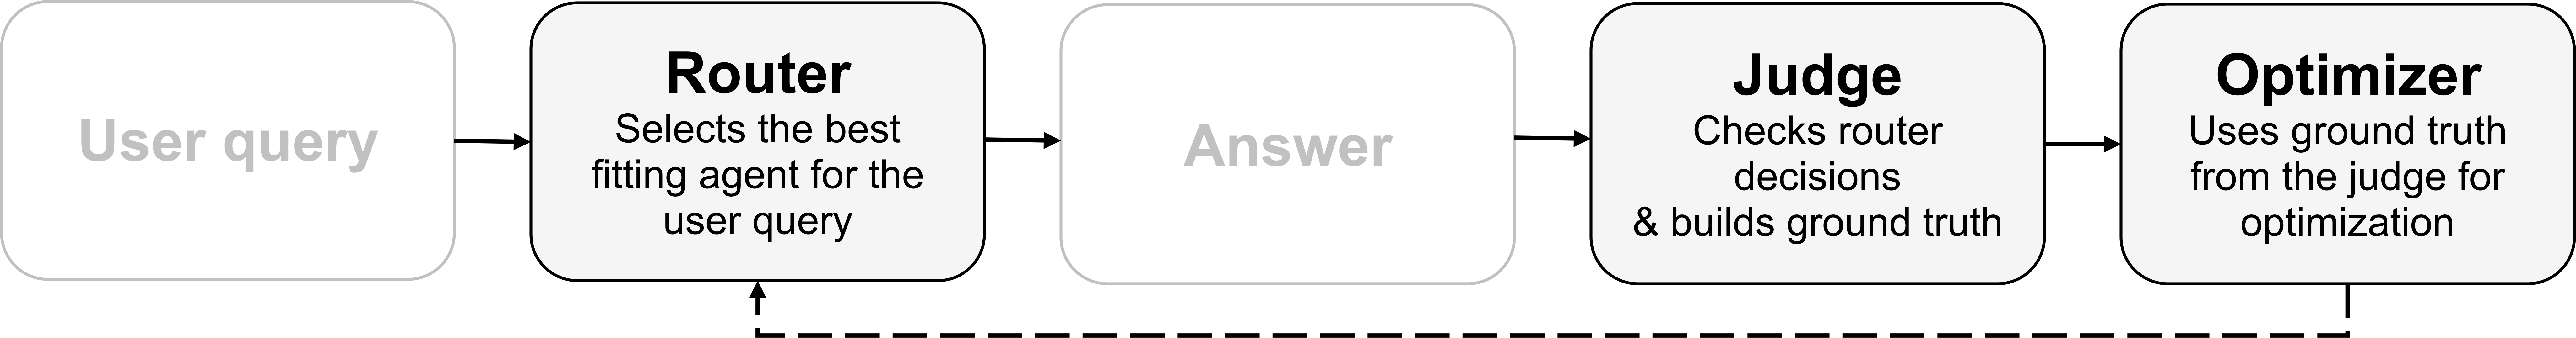
\includegraphics[keepaspectratio]{assets/pipeline/pipeline-architecture.png}}
\caption{High-level overview of the pipeline architecture (own illustration)}
\label{fig:pipeline-architecture}
\end{figure}


The resulting pipeline consists of three components with clearly separated responsibilities. The router makes the routing decision, the judge evaluates it, and the optimizer uses the judge's evaluations to improve the router's system prompt. Evaluation and improvement were deliberately split into two distinct modules rather than one component handling both. This aligns with the modularity principle used throughout the project (see \cref{sec:chatbot-application}) and reflects the design philosophy of \textcite{khattab2024dspy}, whose DSPy framework splits language model pipelines into small, specialized modules instead of components combining several tasks. The separation also keeps the judge's output reusable. The reasoning can later serve both as an evaluation record for humans and as the input signal for the optimizer. The following sections describe the three components in more detail.

\subsection{Router}\label{sec:router}

The preceding sections introduced the eight specialist agents of the PropDesk scenario, each with its own instructions, domain knowledge, and, in production, its own tools and data access. The router assigns every incoming broker query to exactly one of these agents. Queries that fit no specialist domain fall by design to GeneralPurpose, keeping the problem a closed eight-class classification. Misclassification is expensive, since a misrouted specialist returns an answer useless to the advisor. The router must produce a score for each agent and select the highest, so the central design question is how these eight scores are computed. Candidate mechanisms range from asking a model to state its own confidence to measuring semantic similarity, and they differ considerably along the success criteria the project scope fixed before the first sprint, namely accuracy, latency, and cost (see \cref{sec:introduction}). A mechanism that maximizes one dimension while ignoring the other two was ruled out.

\subsubsection{Routing Mechanisms Considered}\label{sec:router-mechanisms}

The candidate mechanisms draw on two largely separate research strands. One strand studies how language models assess their own reliability \autocite{kadavath2022,tian2023,xiong2024}. The other studies how queries are routed between models, typically with dedicated classifiers trained on preference or performance data \autocite{ong2024,chen2023}. Using a model's own confidence signal as routing criterion sits between these strands and is comparatively unexplored, so no established default existed. We therefore analyzed four candidates.

Verbalized confidence asks the routing model to state a confidence value per agent in plain text. It requires no infrastructure change, and our initial system routed exclusively this way, making it the natural baseline. The literature, however, speaks against it as a permanent solution. Models tuned with human feedback verbalize systematically overconfident scores \autocite{tian2023}, and the stated values fluctuate with minor changes in prompt wording \autocite{xiong2024}. A router built on this signal inherits both defects, and our own early tests pointed in the same direction.

Self-consistency samples the router several times at nonzero temperature and scores each agent by the fraction of samples that select it \autocite{wang2023}. The approach is robust and needs no model internals, but multiplies cost and latency by the sample count. Its value also lies in aggregating sampled reasoning chains. A routing decision, however, is a single token, and sampling one token merely approximates the distribution that a single forward pass with token probabilities provides exactly.

Log probabilities read that distribution directly. The routing prompt fixes the answer format to a single token identifying one agent, and the probabilities of the eight admissible tokens are taken from the model's prediction layer instead of its generated text. The result is deterministic, arrives in one forward pass, and contains the full distribution over all eight candidates. Signals read from model internals are also those for which \textcite{kadavath2022} report the most reliable calibration. The drawback is technical, since the serving stack must expose token-level log probabilities.

Embedding similarity involves no language model reasoning at all. The query is embedded once and compared to reference material per agent, at a cost several orders of magnitude below an LLM call. This simplicity is also its weakness. A purely semantic match resolves queries whose intent is semantically unambiguous but fails where the surface form resembles the wrong agent.

\Cref{tbl:mechanisms} compares the four options against the three criteria. None satisfies all of them alone. Verbalized confidence and self-consistency are dominated, while embedding similarity and log probabilities are complementary, which led to combining the latter two in a cascade in the spirit of FrugalGPT, where a cheap mechanism answers what it can answer safely and only the remainder passes to an expensive one \autocite{chen2023}. Stage 1 routes by semantic recognition, Stage 2 deliberates over the cases recognition cannot settle (see \cref{fig:pipeline}), following the dual-process idea of \textcite{kahneman2011}. The verbalized-only router remained in place as the comparison point for \cref{sec:empirical-evaluation}.

\begin{longtable}[]{@{}
  >{\raggedright\arraybackslash}p{(\linewidth - 8\tabcolsep) * \real{0.2442}}
  >{\raggedright\arraybackslash}p{(\linewidth - 8\tabcolsep) * \real{0.2674}}
  >{\raggedright\arraybackslash}p{(\linewidth - 8\tabcolsep) * \real{0.1279}}
  >{\raggedright\arraybackslash}p{(\linewidth - 8\tabcolsep) * \real{0.1279}}
  >{\raggedright\arraybackslash}p{(\linewidth - 8\tabcolsep) * \real{0.2326}}@{}}
\caption{The four candidate mechanisms against the success criteria of \cref{sec:introduction} (own illustration).}\label{tbl:mechanisms}\tabularnewline
\toprule\noalign{}
\begin{minipage}[b]{\linewidth}\raggedright
Mechanism
\end{minipage} & \begin{minipage}[b]{\linewidth}\raggedright
Score quality
\end{minipage} & \begin{minipage}[b]{\linewidth}\raggedright
Latency
\end{minipage} & \begin{minipage}[b]{\linewidth}\raggedright
Cost
\end{minipage} & \begin{minipage}[b]{\linewidth}\raggedright
Key limitation
\end{minipage} \\
\midrule\noalign{}
\endfirsthead
\toprule\noalign{}
\begin{minipage}[b]{\linewidth}\raggedright
Mechanism
\end{minipage} & \begin{minipage}[b]{\linewidth}\raggedright
Score quality
\end{minipage} & \begin{minipage}[b]{\linewidth}\raggedright
Latency
\end{minipage} & \begin{minipage}[b]{\linewidth}\raggedright
Cost
\end{minipage} & \begin{minipage}[b]{\linewidth}\raggedright
Key limitation
\end{minipage} \\
\midrule\noalign{}
\endhead
\bottomrule\noalign{}
\endlastfoot
Verbalized confidence & low, overconfident & 1 LLM call & 1 LLM call & unreliable signal \\
Self-consistency & medium, robust & k LLM calls & k LLM calls & k-fold overhead \\
Log probabilities & high, full distribution & 1 LLM call & 1 LLM call & needs logprob access \\
Embedding similarity & high if unambiguous & ms & negligible & fails on ambiguity \\
\end{longtable}

\begin{figure}
\centering
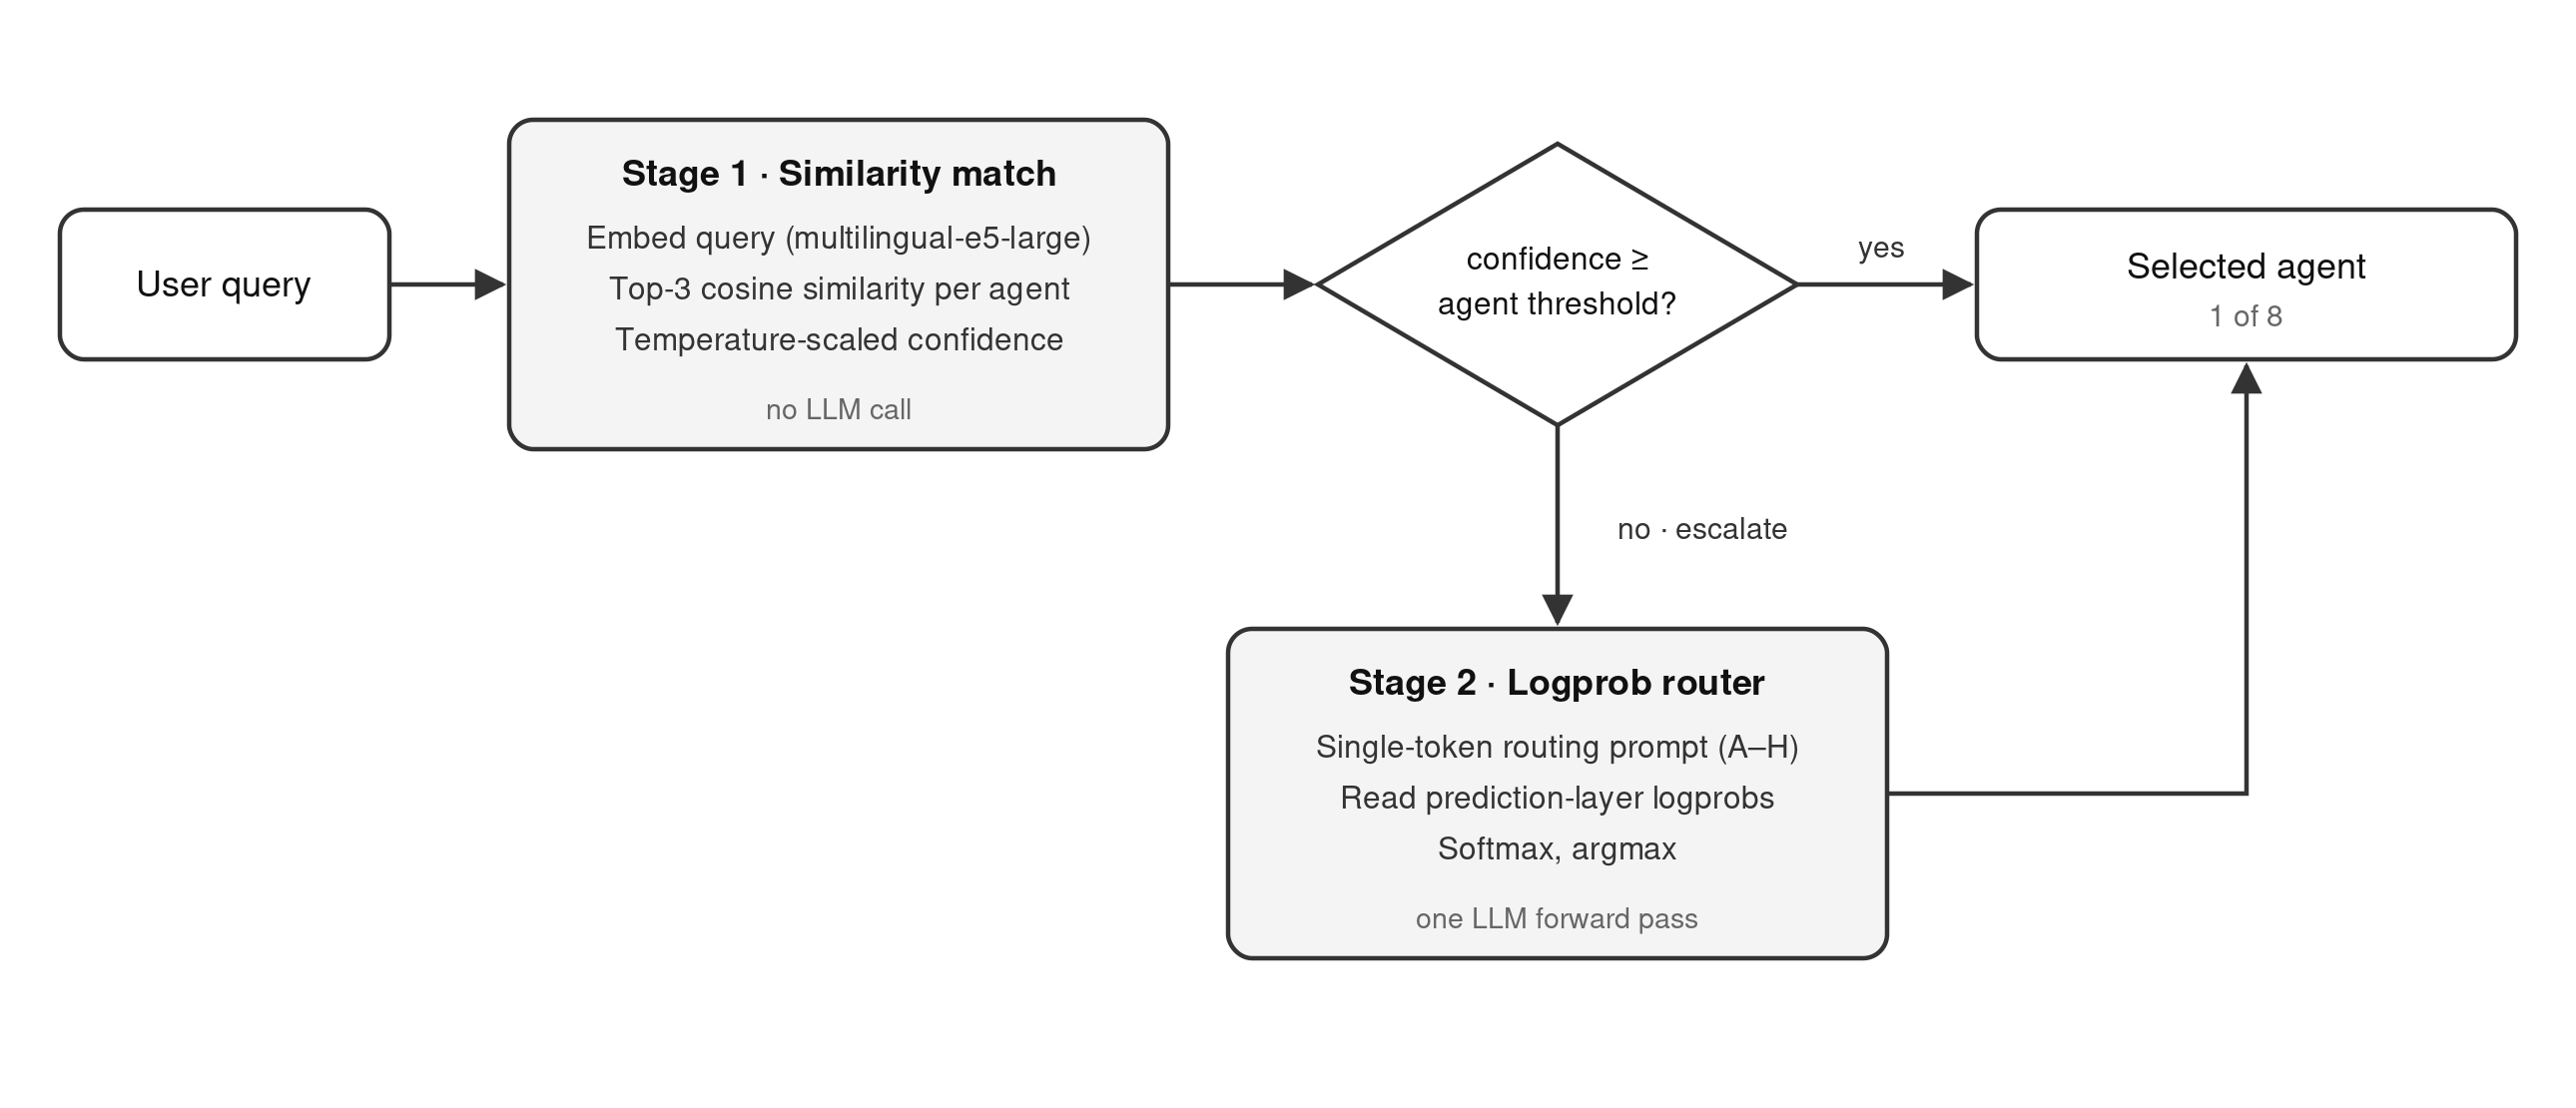
\includegraphics[width=1\linewidth,height=\textheight,keepaspectratio]{assets/router/fig-4-1-two-stage-pipeline.png}
\caption{Two-stage routing pipeline. Stage 1 resolves recognizable queries without an LLM call, Stage 2 deliberates over escalated cases (own illustration).}\label{fig:pipeline}
\end{figure}

\subsubsection{Stage 1, Routing by Semantic Similarity}\label{sec:router-stage1}

Stage 1 rests on a vector store of labeled reference queries, each stored with its embedding and agent label. The store is seeded from the golden dataset and grows through judge-confirmed production traces (\cref{sec:judge}). An incoming query is embedded with multilingual-e5-large, a self-hosted model producing 1024-dimensional vectors \autocite{wang2024}. Broker queries arrive in German and English, often mixed within one conversation, and the multilingual model maps both into one shared vector space, so a German query can match an English reference about the same task. Self-hosting keeps embedding cost independent of query volume and query content on our own infrastructure.

Each agent is scored by the mean cosine similarity between the query vector and its three closest reference queries. Our first design condensed every agent into a single centroid vector. This proved too coarse. An agent such as GeneralPurpose covers heterogeneous subtasks whose embeddings share no common center, and averaging them yields a representative vector that reflects none of them well. Scoring against individual reference queries preserves this local structure, so the instance-based variant replaced the centroid.

Raw cosine scores proved unsuitable as a decision signal. Embedding spaces are anisotropic, meaning the vectors concentrate in a narrow cone, which compresses all similarities into a tight band and makes absolute values hard to interpret \autocite{ethayarajh2019,steck2024}. All embeddings are therefore centered by subtracting the mean vector of the reference store and renormalizing, which spreads the similarity distribution. On top of that, we considered three variants of the decision signal. Variant A uses the raw margin between best and second-best agent score, Variant B the same margin on centered embeddings, and Variant C a temperature-scaled softmax over the per-agent scores, using the top-agent probability, with the temperature fitted on calibration data by minimizing negative log-likelihood \autocite{guo2017}. We selected Variant C on conceptual grounds rather than a measured accuracy difference. A probability between zero and one can be monitored directly, remains comparable across agents, and costs nothing mathematically, since temperature scaling provably cannot alter the agent ranking.

Whether Stage 1 may route directly is governed by calibrated thresholds. We fixed an error budget of five percent for directly routed queries and determined, per agent, the lowest confidence threshold at which the empirical error on held-out calibration data (1,000 queries, at least 50 per agent) stays within that budget. This follows conformal calibration, which converts a held-out sample into distribution-free error control \autocite{angelopoulos2023}. Thresholds are fitted per agent because score distributions differ substantially between agents. The fitted values range from 33.5 percent for GeneralPurpose to 94.2 percent for PlatformSupport. An agent falling below ten calibration samples reverts to a pooled global threshold. Because centering mean and score distribution shift as the store grows, thresholds are refitted periodically after judge-loop extensions (\cref{sec:judge}). \Cref{fig:risk-coverage} shows the resulting risk-coverage curve, with the deployed operating point at 96 percent coverage and 4.9 percent risk, inside the budget.

\begin{figure}
\centering
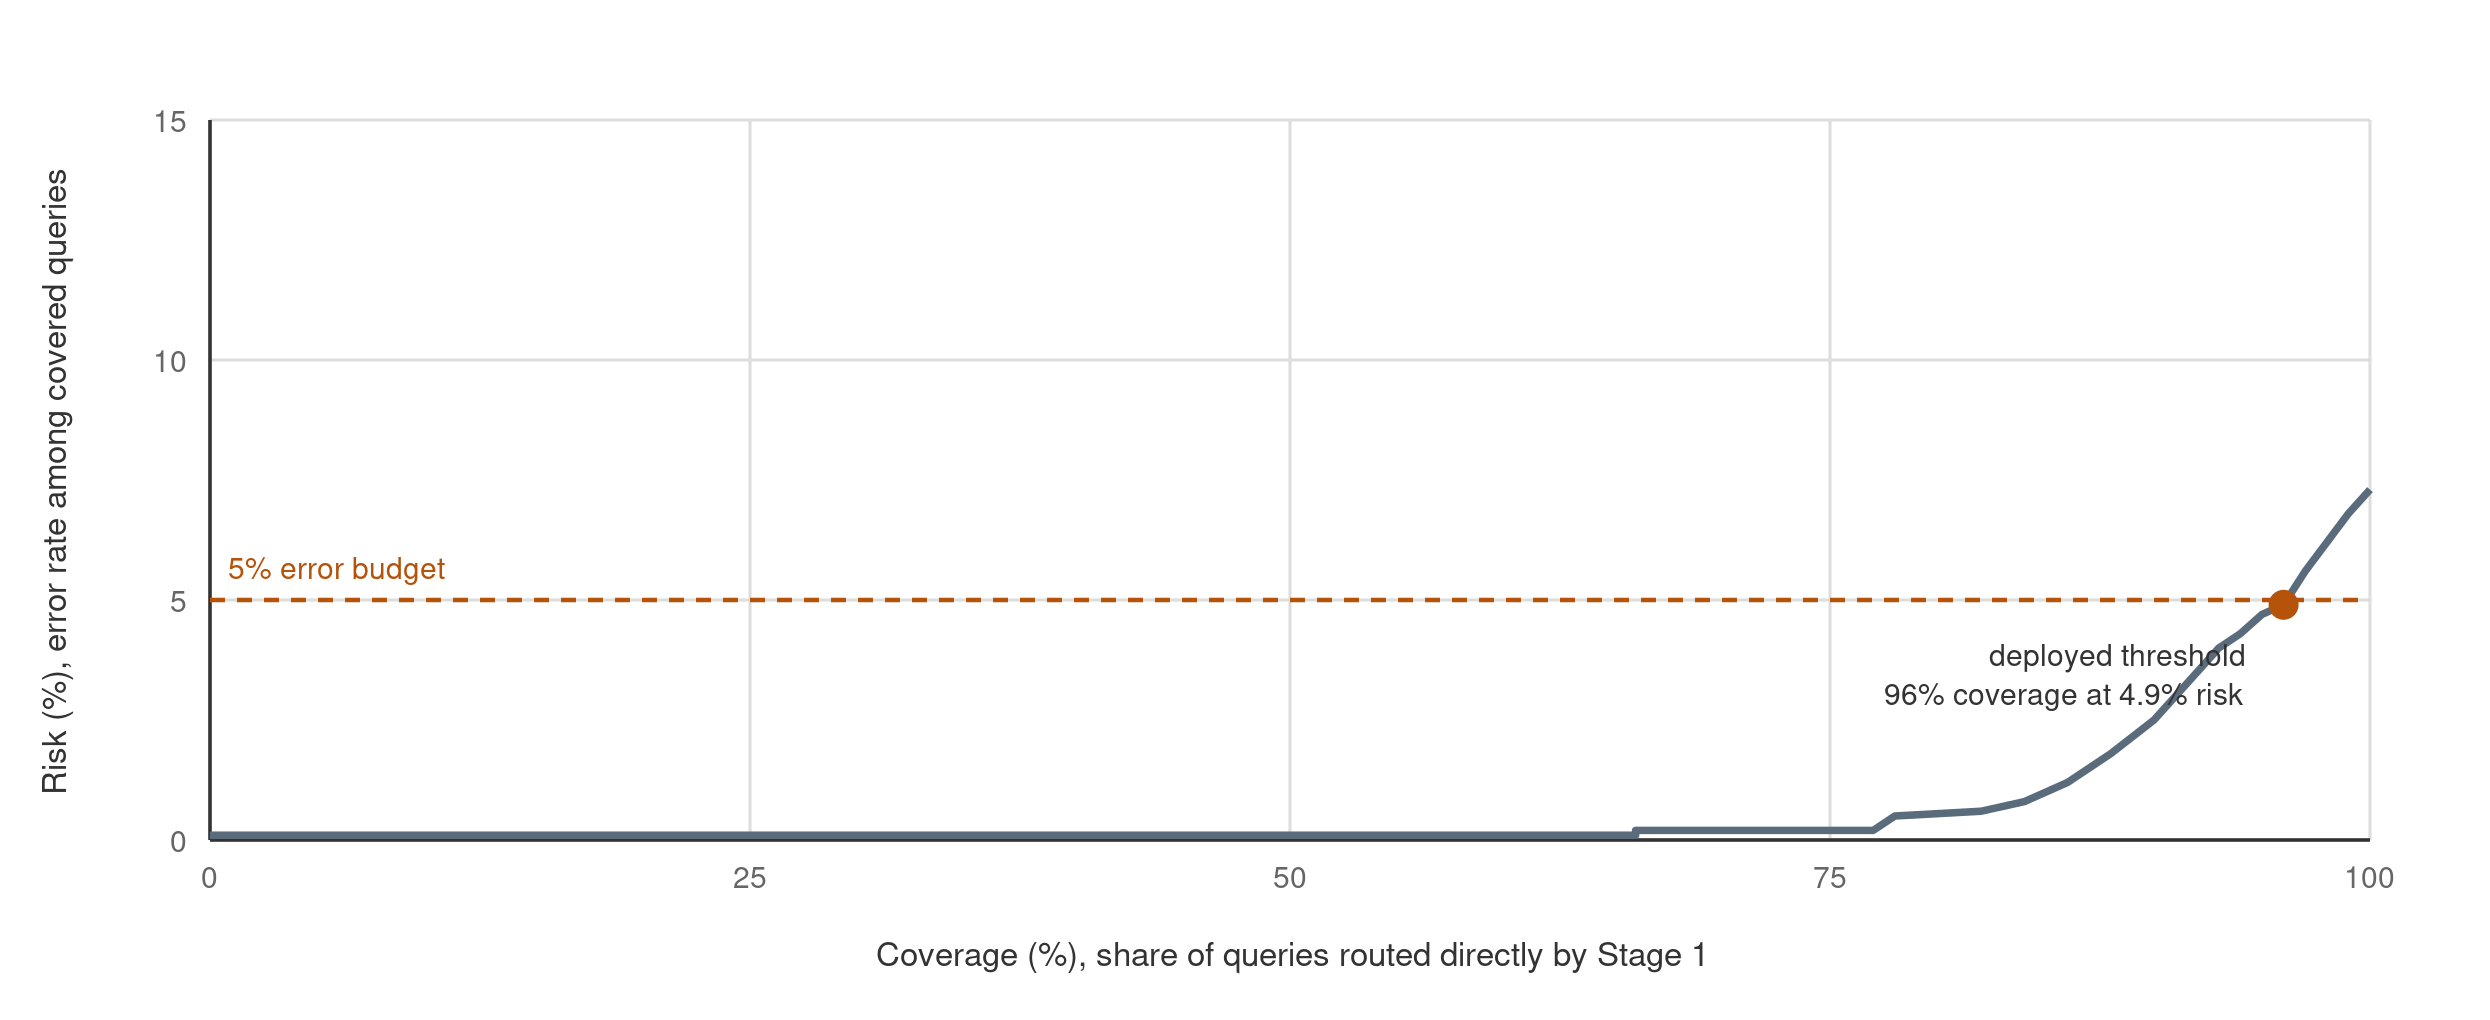
\includegraphics[width=1\linewidth,height=\textheight,keepaspectratio]{assets/router/fig-4-2-risk-coverage.png}
\caption{Risk-coverage curve of the calibrated Stage 1 router on held-out calibration data. The deployed operating point covers 96 percent of queries at 4.9 percent risk (own illustration).}\label{fig:risk-coverage}
\end{figure}

To protect the validity of this procedure, reference store and calibration set are disjoint, near-duplicates (similarity 0.99 or higher) are excluded as self-matches, and coverage and risk are estimated with five-fold cross-conformal validation rather than on the fitting data. A query that clears its agent's threshold is routed directly. Everything else escalates, which turns Stage 1 into a selective classifier that abstains whenever its confidence is insufficient \autocite{geifman2017}. In code, the decision reduces to two lines, all learned quantities loaded as configuration (\cref{fig:stage1-code}).

\begin{figure}
\centering
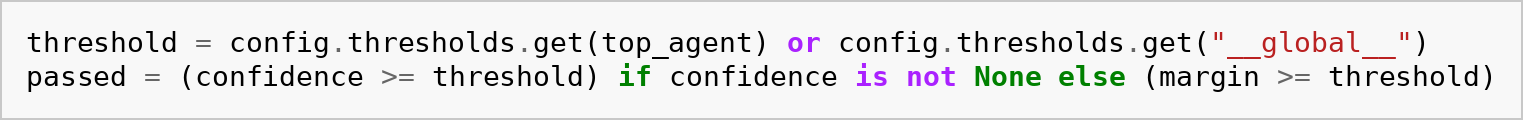
\includegraphics[width=1\linewidth,height=\textheight,keepaspectratio]{assets/router/fig-4-3-stage1-decision-rule.png}
\caption{Stage 1 decision rule, calibrated confidence against the per-agent threshold (\protect\texttt{router.py}).}\label{fig:stage1-code}
\end{figure}

\subsubsection{Stage 2, Routing by Log Probabilities}\label{sec:router-stage2}

Queries that Stage 1 abstains from escalate to a Gemma 4 E4B model, served locally through Ollama and dedicated to routing. The eight agents are encoded as fixed single-token identifiers, the letters A through H, and the routing prompt instructs the model to answer with exactly one of them. Instead of sampling that answer, we request the top log probabilities alongside the generated token and read the admissible route codes directly from the prediction layer. These are renormalized over the observed codes. A code missing from the returned candidates receives zero probability, a slight truncation bias we accept for simplicity. One forward pass thus yields a deterministic distribution over all eight agents, which matters for reproducible evaluation. Stage 2 always routes to its top candidate. As the final stage it has no abstention option, and its probabilities enter the decision uncalibrated, resting on the reliability that \textcite{kadavath2022} report for internal signals. The distribution is logged in full with every trace. Its runner-up later lets the judge compare the chosen agent against the strongest alternative (\cref{sec:judge}). The routing prompt is versioned so that the optimizer can improve it over time (\cref{sec:optimizer}), making it data rather than code, and the model sits behind a provider interface, so a different routing model requires a new provider class and no change to the dispatch logic.

The routing call generates exactly one token and asks the runtime for the log probabilities of the most likely tokens, from which the route codes are extracted and renormalized (\cref{fig:stage2-code}).

\begin{figure}
\centering
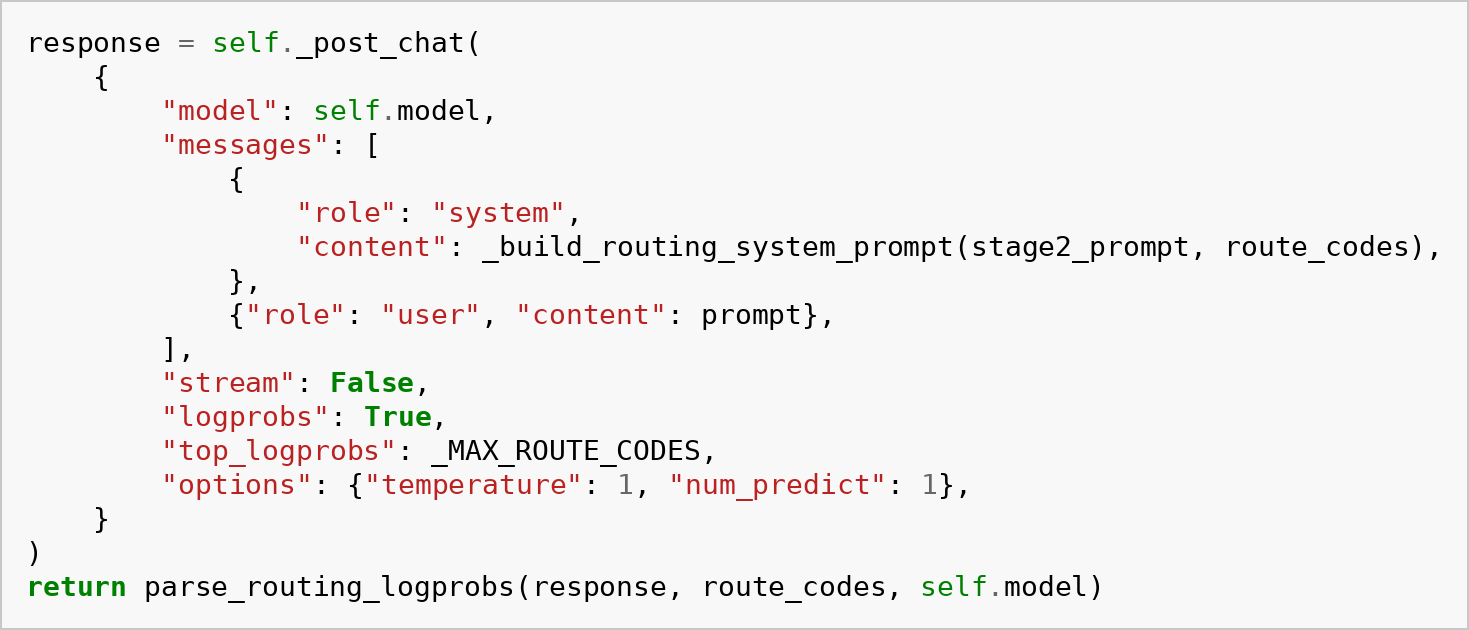
\includegraphics[width=0.9\linewidth,height=\textheight,keepaspectratio]{assets/router/fig-4-4-stage2-routing-call.png}
\caption{Stage 2 routing call, one generated token with token-level log probabilities (\protect\texttt{providers/ollama.py}, shortened for presentation).}\label{fig:stage2-code}
\end{figure}

\subsubsection{Integrated Workflow and Reflection}\label{sec:router-workflow}

At dispatch time the router loads the active configuration, embeds the query, and runs Stage 1. If the calibrated confidence clears the threshold, the selected agent answers immediately. Otherwise Stage 2 decides. Every trace records the path taken, both stages' scores, and all latencies (\cref{fig:dispatch-flow}).

\begin{figure}
\centering
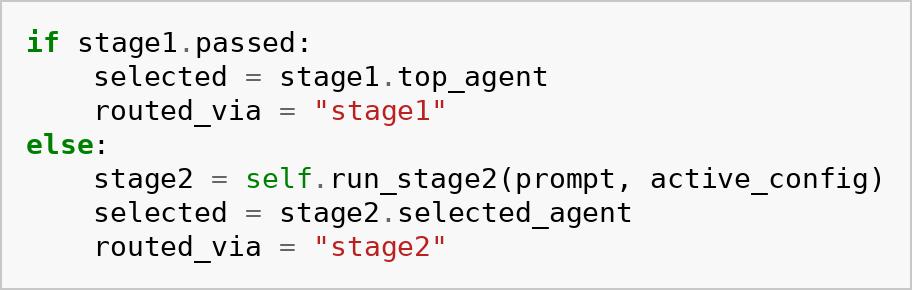
\includegraphics[width=0.75\linewidth,height=\textheight,keepaspectratio]{assets/router/fig-4-5-dispatch-flow.png}
\caption{Escalation logic in the dispatch flow (\protect\texttt{router.py}).}\label{fig:dispatch-flow}
\end{figure}

Compared to the initial system, which sent every query to an LLM and trusted its verbalized confidence, the two-stage design changes the operating characteristics in three ways. On the calibration distribution, 96 percent of queries never reach a language model, which cuts LLM calls and brings average latency down to embedding speed. Accuracy is nevertheless preserved, because Stage 1 only decides where its calibrated error stays within budget and hands every ambiguous case to the stronger mechanism. And the confidence signal is now read from model internals and calibrated on data instead of being stated by the model about itself. The system degrades gracefully, as Stage 1 still produces a ranked decision if the LLM runtime is unavailable. \Cref{sec:empirical-evaluation} quantifies these effects.

Some limitations remain. First, the calibrated thresholds guarantee the error budget only for the distribution of the calibration data, which is synthetic, so production drift requires recalibration. The long-run behavior of the judge loop that provides it was not observed within the project timeframe. Second, all findings rest on one embedding model and one routing model family, and the ranking of mechanisms could shift for models with differently calibrated logits. Third, the log-probability design presupposes a serving stack that exposes token-level probabilities, which restricts the choice of inference runtimes. Fourth, Stage 2 has no abstention option and routes on uncalibrated probabilities. A second selective layer, such as a clarifying question to the broker, remains future work.

\subsection{Judge}\label{sec:judge}

\subsubsection{Role in the Pipeline}\label{sec:judge-role}

Building upon the LLM-as-a-judge paradigm introduced in \cref{sec:pipeline-justification}, this section explains the judge's operational role within the pipeline. As the judge operates directly on unlabelled production queries, it builds up a golden dataset over time and removes the need to construct and maintain a synthetic test set for evaluation. Furthermore, it produces a structured failure analysis that would otherwise demand a manual root-cause analysis.

As described in \cref{sec:router}, the router produces a full candidate ranking over all eight agents, from which the second-best candidate can be identified. In the live environment, the selected agent directly returns a response to the user. The judge is given the response of the selected agent and a counterfactual response generated by calling the second-ranked candidate with the same query and produces a verdict with justification explaining which one better resolves it. Depending on which stage of the router made the routing decision, this verdict is either written directly into the example store for Stage 1 or passed on to the optimizer. The detailed mechanism behind this distinction is described in \cref{sec:judge-implementation}. \Cref{fig:judge-role} illustrates the general flow.

\begin{figure}
\centering
\pandocbounded{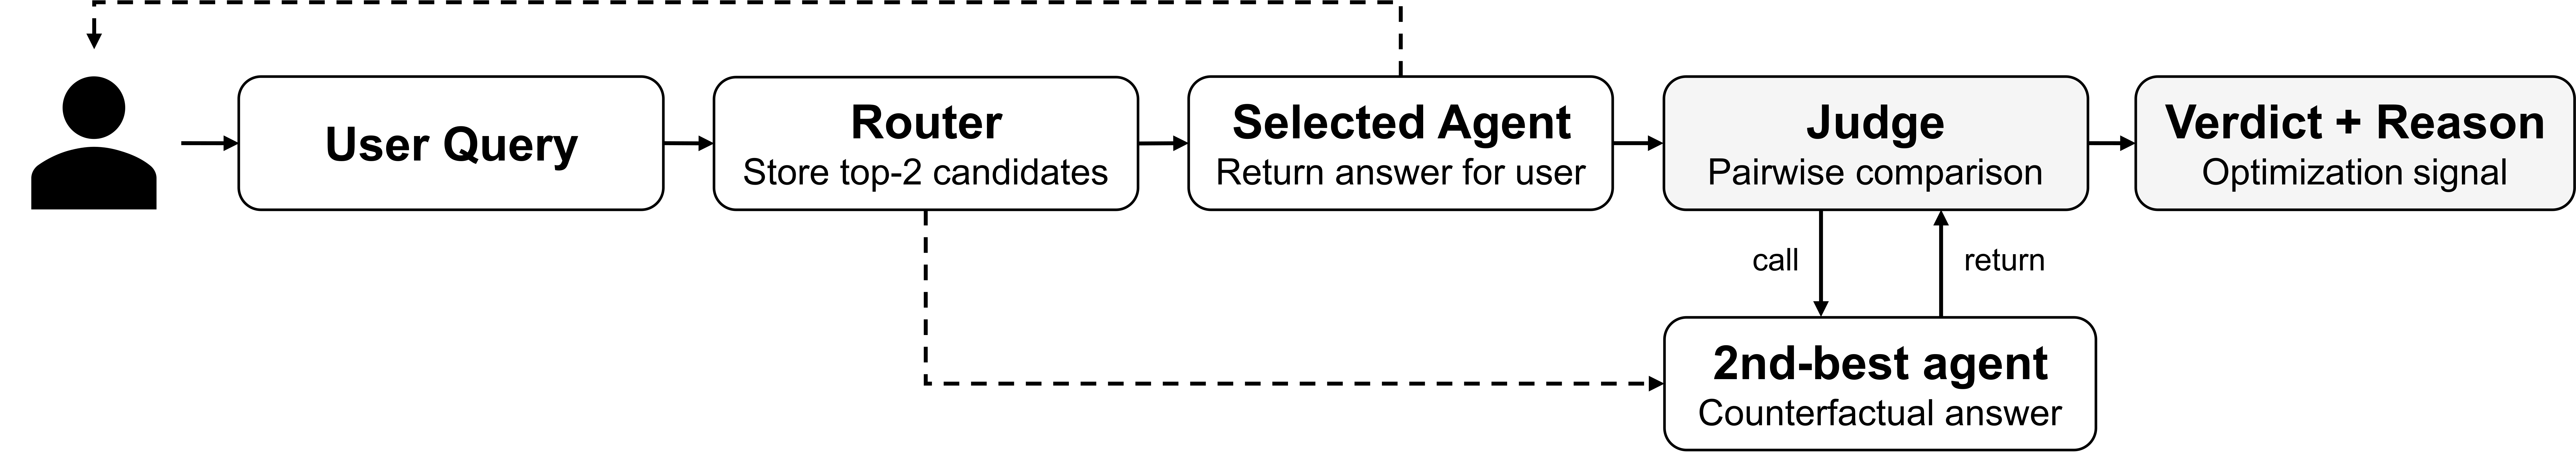
\includegraphics[keepaspectratio]{assets/pipeline/judge-role.png}}
\caption{Role of the judge component within the pipeline.}
\label{fig:judge-role}
\end{figure}


The comparison is restricted to the top two candidates rather than all eight agents. This is a practical decision grounded in empirical observation. The score margin between the second- and third-ranked agent is typically larger than between the first- and second-ranked one, so routing ambiguity is almost always a decision between the top two agents. Restricting the comparison ensures the evaluation of relevant cases and avoids the cost of additional candidate responses but comes at the risk of missing a correct agent ranked lower. In ambiguous cases the judge therefore considers a third agent, which is described in more detail in Section 4.3.3.

For the format of the evaluation generally two different formats exist. In a pointwise evaluation, each response is scored independently, and the scores are compared afterward. In a comparative format the judge sees all candidates at once and decides directly. Comparative evaluation was adopted for two reasons. First, it lets the judge weigh a response against the concrete alternative that was actually available, which \textcite{zheng2023judging} identify as more suitable for this kind of preference decision, and because it is more efficient, resolving the comparison in a single call instead of one call per response plus a separate comparison step.

The reasoning generated with the verdict is essential for closing the optimization loop. A binary correct/incorrect flag only indicates performance but fails to explain why a decision was correct or not. The judge's reasoning provides the optimizer with the context required to identify systemic failure patterns and refine the router's system prompt \autocite{yang2023llmoptimizers}.

\subsubsection{Bias Mitigation and Evaluation Results}\label{sec:judge-bias}

As the judge's verdict functions as the system's ground truth for the router's routing decisions, its reliability is critical, since errors would propagate through the pipeline. Research shows that an LLM judge is not a neutral instrument. It is prone to systematic biases that can shift its verdicts independently of the actual answer quality \autocite{gu2024llmjudge}. This section covers the biases relevant for this project, how they were mitigated, and how the mitigations affected the evaluation results of the judge.

One bias that could plausibly affect the judge is identity bias, where a judge's verdict is influenced by knowing which agent generated which answer, rather than by the content of the answers themselves \autocite{koo2023biases}. If the judge is aware, for example, that a response was generated by the MarketInfoAgent, it might favor the response because the query touches on market information, regardless of whether the response itself is the better answer. Consistent with the anonymized comparison approach used by \textcite{koo2023biases}, this bias is addressed by evaluating the two candidate answers blindly. Each is assigned a letter (A or B) in place of the agent's name. The judge sees and outputs only these letters, the mapping back to the actual agent is resolved once the verdict is returned.

A second bias is position bias, which is the tendency of the judge to favor a response because of where it appears in the prompt, rather than because of its content \autocite{zheng2023judging}. To mitigate this bias, the order in which the judge receives the agent responses is randomized, since the router's selected agent would otherwise always appear first.

To fine-tune the judge module and monitor its behavior over time, an evaluation dashboard tracking overall accuracy, how often the judge corrects or introduces router errors, and how often it confuses one agent with another, was built. It also reports the verdict distribution across positions A and B, and accuracy by position, as a direct check for position bias. The evaluation used a subset of the golden dataset introduced in \cref{sec:initial-project-setup}, namely the 100 queries where the router's routing was wrong or most uncertain, chosen to allow fast iteration before evaluating on the full dataset and to tune the judge on a small subset before evaluating it on the full dataset. The first evaluation used Gemma 4 31B with a basic comparison prompt. \Cref{fig:judge-basic-prompt} displays the results of the initial evaluation.

\begin{figure}
\centering
\pandocbounded{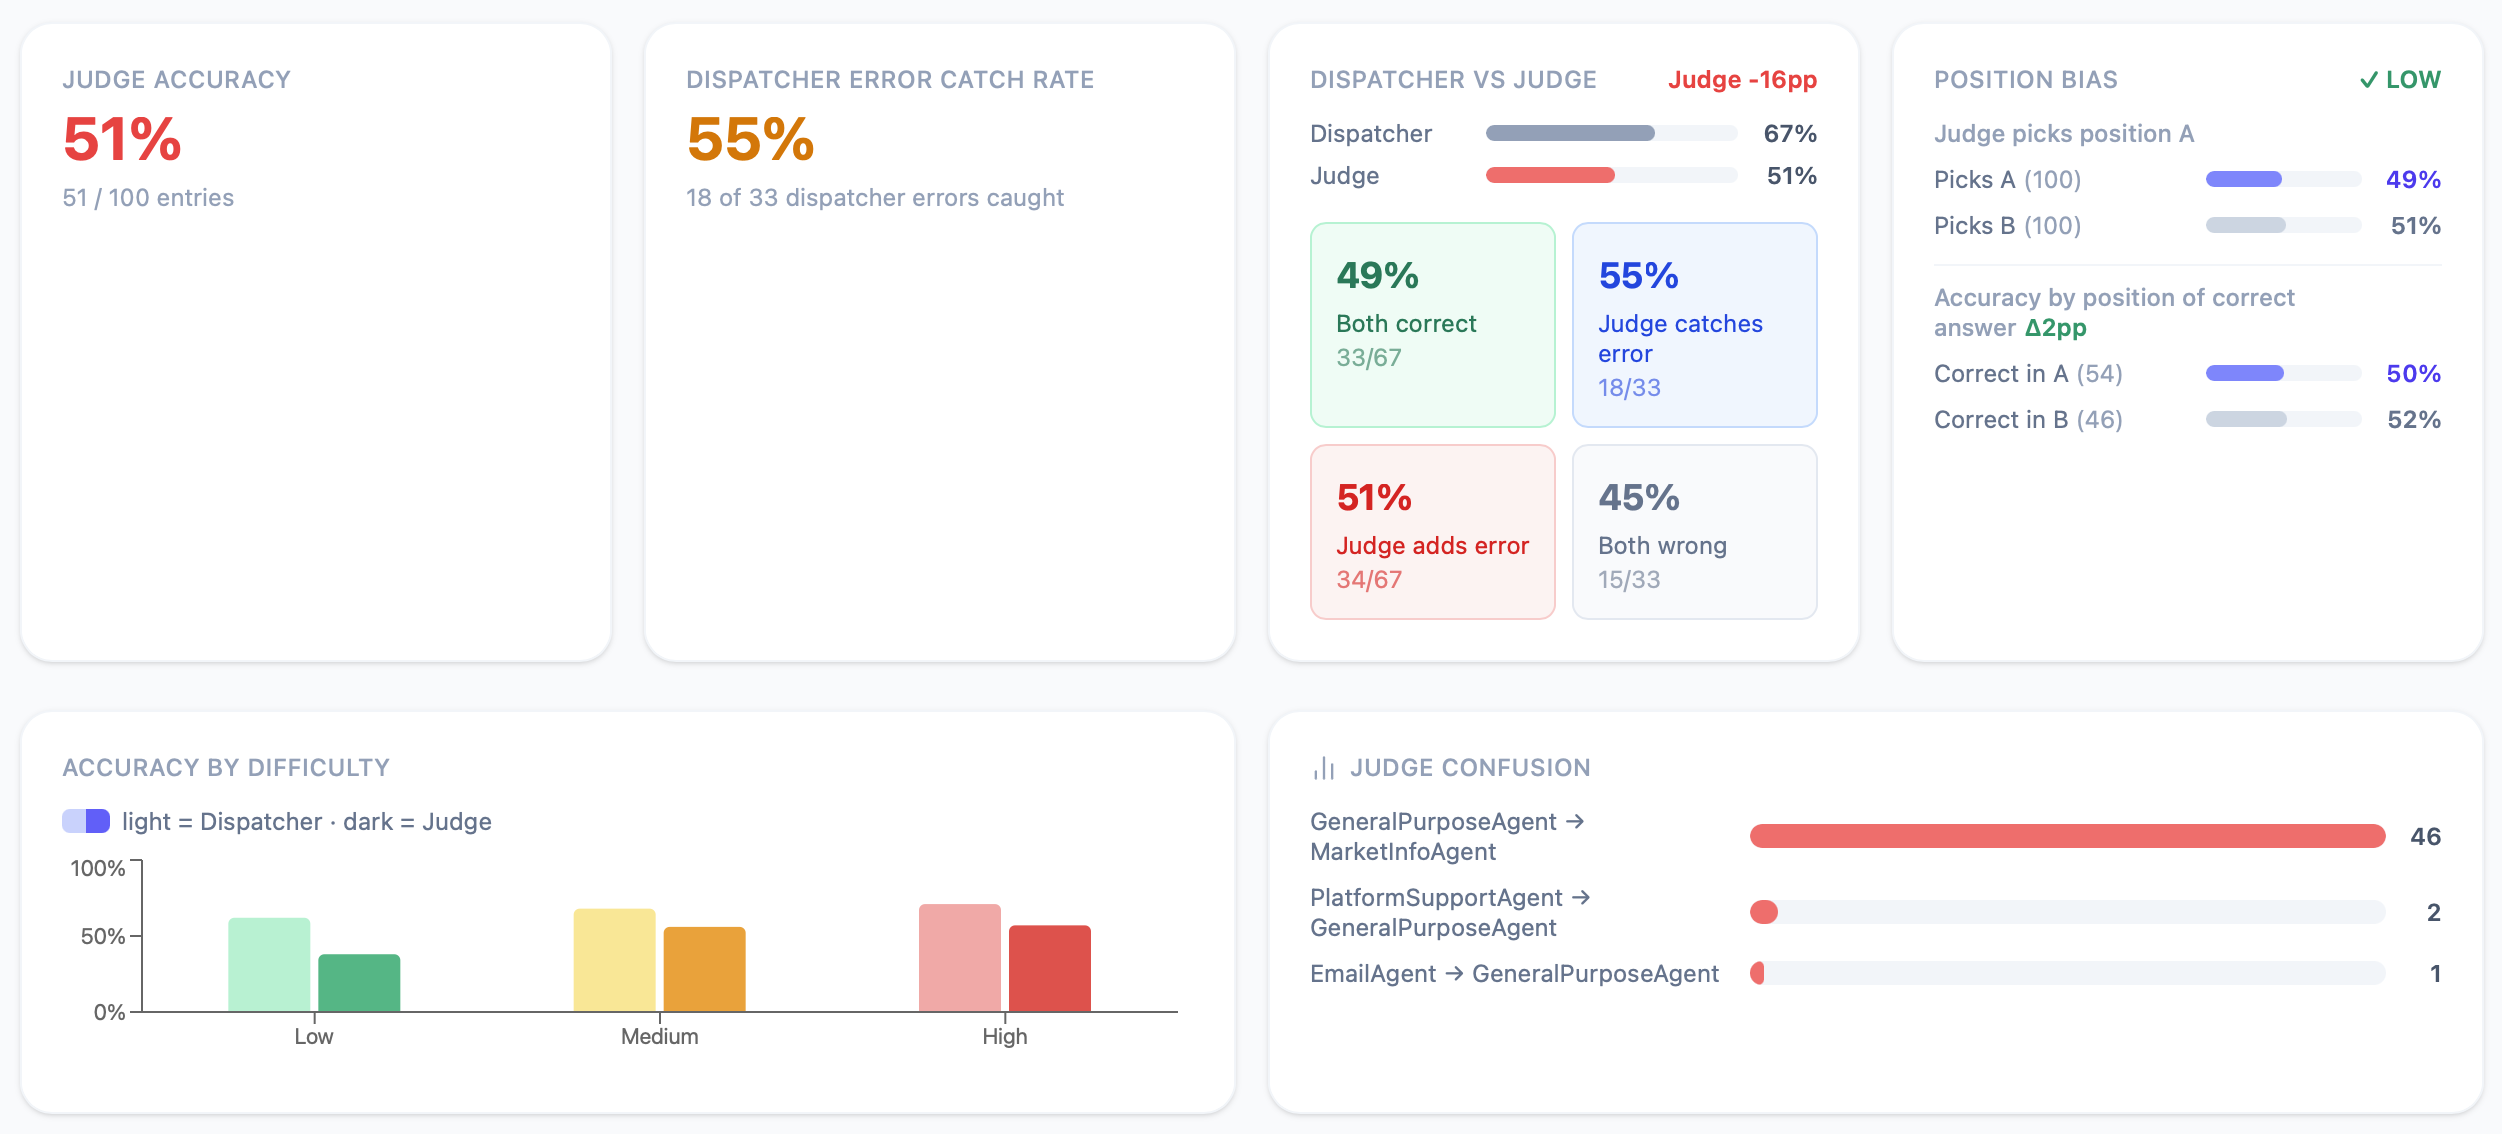
\includegraphics[keepaspectratio]{assets/pipeline/fig3_dashboard_basic_prompt.png}}
\caption{Judge evaluation on the training dataset using Gemma4 31b and a basic comparison prompt.}
\label{fig:judge-basic-prompt}
\end{figure}


The dashboard shows a position distribution close to even, with no indication of a position bias. This finding does not make the mitigation unnecessary. A systematic study by \textcite{shi2024positionbias} confirms that the direction and strength of the position bias vary across judge models and tasks, so the safeguard remains relevant for future model changes.

The results show a judge agreement of 51\% with the ground truth dataset, which is rarely better than chance for a binary decision. The confusion metric revealed a recurring pattern. The judge systematically preferred MarketInfoAgent responses over those from the GeneralPurposeAgent, even when the router had correctly selected the latter. Inspecting these cases showed that MarketInfoAgent responses were consistently more verbose and included comparison tables, section headers, and a data limitation note, while GeneralPurposeAgent responses tend to be shorter and less structured. The judge interpreted these formatting features as signals of quality rather than style. This is an appearance of style bias, which \textcite{soumik2026biasmitigation} identifies as the dominant bias among LLM judges, compounded by verbosity bias, the tendency to favor longer answers regardless of their actual content \autocite{zheng2023judging}.

Style bias is mitigated through evaluation rubrics, which is a set of explicit, structured criteria the judge applies for its evaluation instead of unconstrainedly performing an overall judgement. The results reported by \textcite{kim2024prometheus} show that fine-grained rubrics let smaller models reach the agreement levels of much larger ones without such rubrics.

The judge's rubric consists of three routing-specific criteria that are the result of iterative testing until the best results were reached. Helpfulness assesses how well the response resolves the broker's actual request. Specificity assesses whether the response reflects the domain knowledge of the appropriate specialized agent and stays within the scope of the query. Conciseness assesses whether the response is as direct as the query requires. The judge is prompted to apply these criteria sequentially rather than all at once. It first produces a short comparative assessment per criterion, evaluating both candidates on one criterion before moving to the next, and only then forms its final verdict and justification. This sequencing follows the chain-of-thought, form-filling approach introduced by \textcite{liu2023geval} for LLM-based evaluation, and makes it harder for a single feature, such as a table, to dominate the outcome.

\begin{figure}
\centering
\pandocbounded{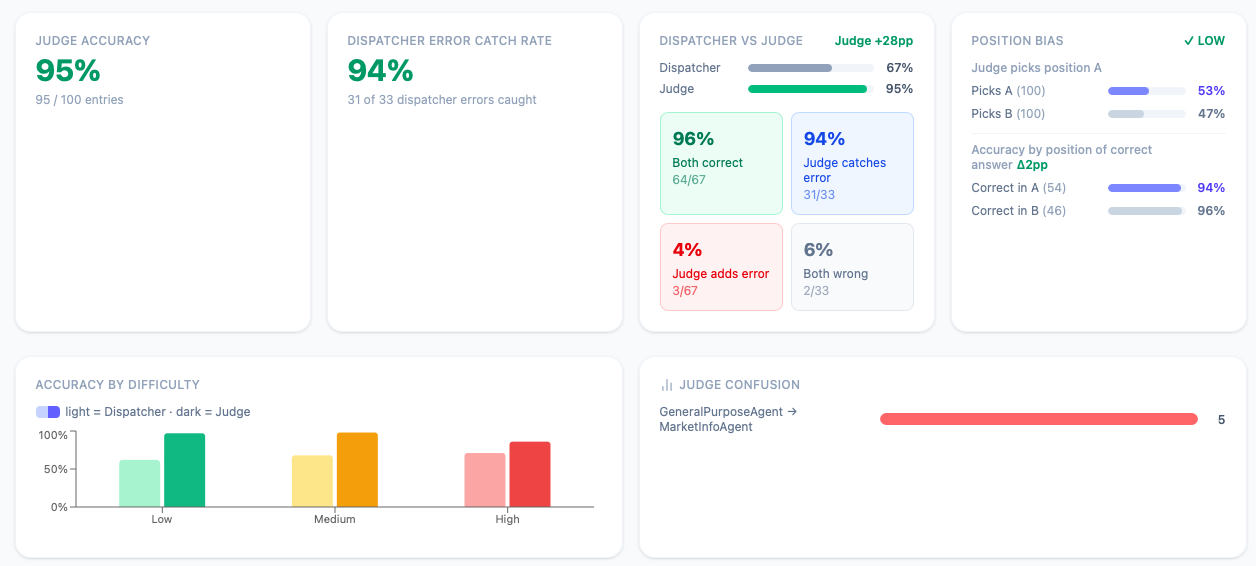
\includegraphics[keepaspectratio]{assets/pipeline/fig4_dashboard_rubrics.png}}
\caption{Judge evaluation on the training dataset using Gemma 4 31b and routing-specific rubrics.}
\label{fig:judge-rubrics}
\end{figure}


Introducing rubrics raised the judge accuracy by 44 percentage points on the dataset with the 100 most uncertain queries (\cref{fig:judge-rubrics}). Once the team gathered access to AWS Bedrock, the judge model was migrated to Claude Sonnet 4.6 and evaluated on the 1,000-query golden dataset to ensure it generalizes on unseen queries.

\begin{figure}
\centering
\pandocbounded{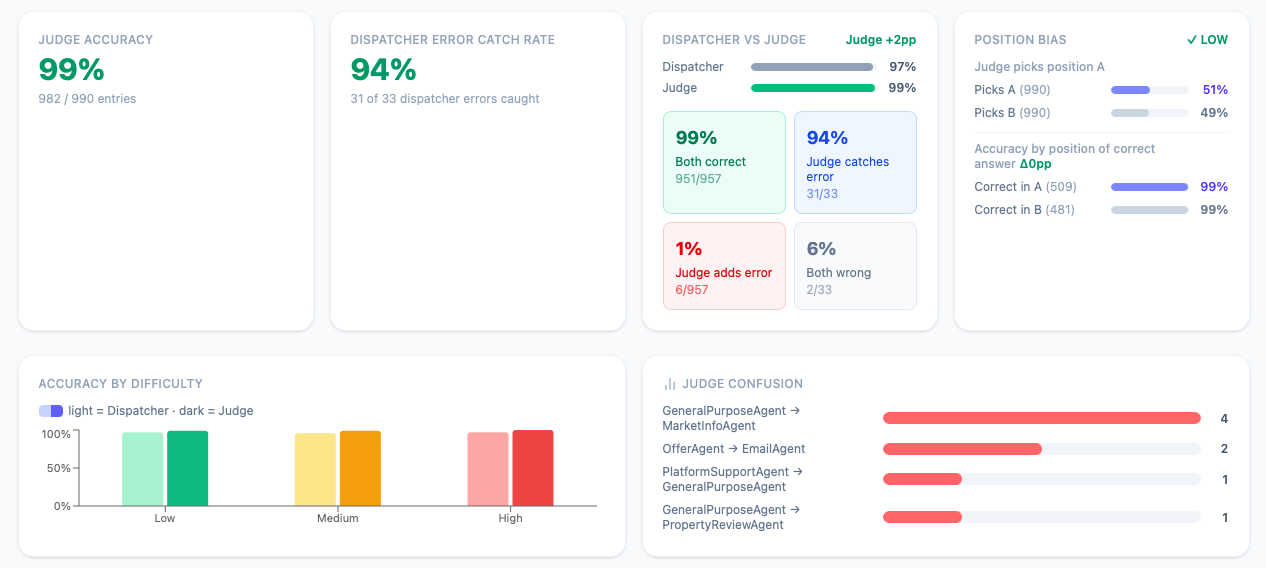
\includegraphics[keepaspectratio]{assets/pipeline/fig5_dashboard_sonnet.png}}
\caption{Judge evaluation on the evaluation dataset using Claude Sonnet 4.6 and routing-specific rubrics.}
\label{fig:judge-sonnet}
\end{figure}


The final evaluation reached 99\% agreement (\cref{fig:judge-sonnet}), confirming the judge is reliable enough to grade the router's decisions. In the evaluation, 10 out of the 1,000 queries were excluded due to API overload during the agent response generation, leading to empty responses returned by the agents.

Another recognized strategy against individual judge biases is replacing the single judge with a panel of models that aggregate their verdicts \autocite{verga2024juries}. Survey work classifies such multi-judge setups among the established mitigation strategies \autocite{gu2024llmjudge}. The option was rejected for this project for multiple reasons. First, costs scale linearly with the panel size, which is the dominant factor for a component running on every query. Second, the benefit of a panel supposes diverse model families, since judges from the same family share the same biases, and aggregation then reinforces these biases rather than cancelling them. A credible cross-family panel was not available within the project's LLM access constraints. Third, each panel member would also require its own prompt engineering and validation, which multiplies the iteration effort documented above beyond what the project's timeline allowed. Given that the single-judge setup already reached 99\% agreement, a panel remains an option in the future only if the judge accuracy drops on newly constructed test queries.

\subsubsection{Implementation}\label{sec:judge-implementation}

The previous sections described how the judge reaches its verdict. This section focuses on the implementation of the judge module from a processual perspective. It describes which steps are taken within the judge module and how the judge verdict flows back into the router's two stages to correct routing decisions and improve future performance. \Cref{fig:judge-process} illustrates the three cases that govern this process.

\begin{figure}
\centering
\pandocbounded{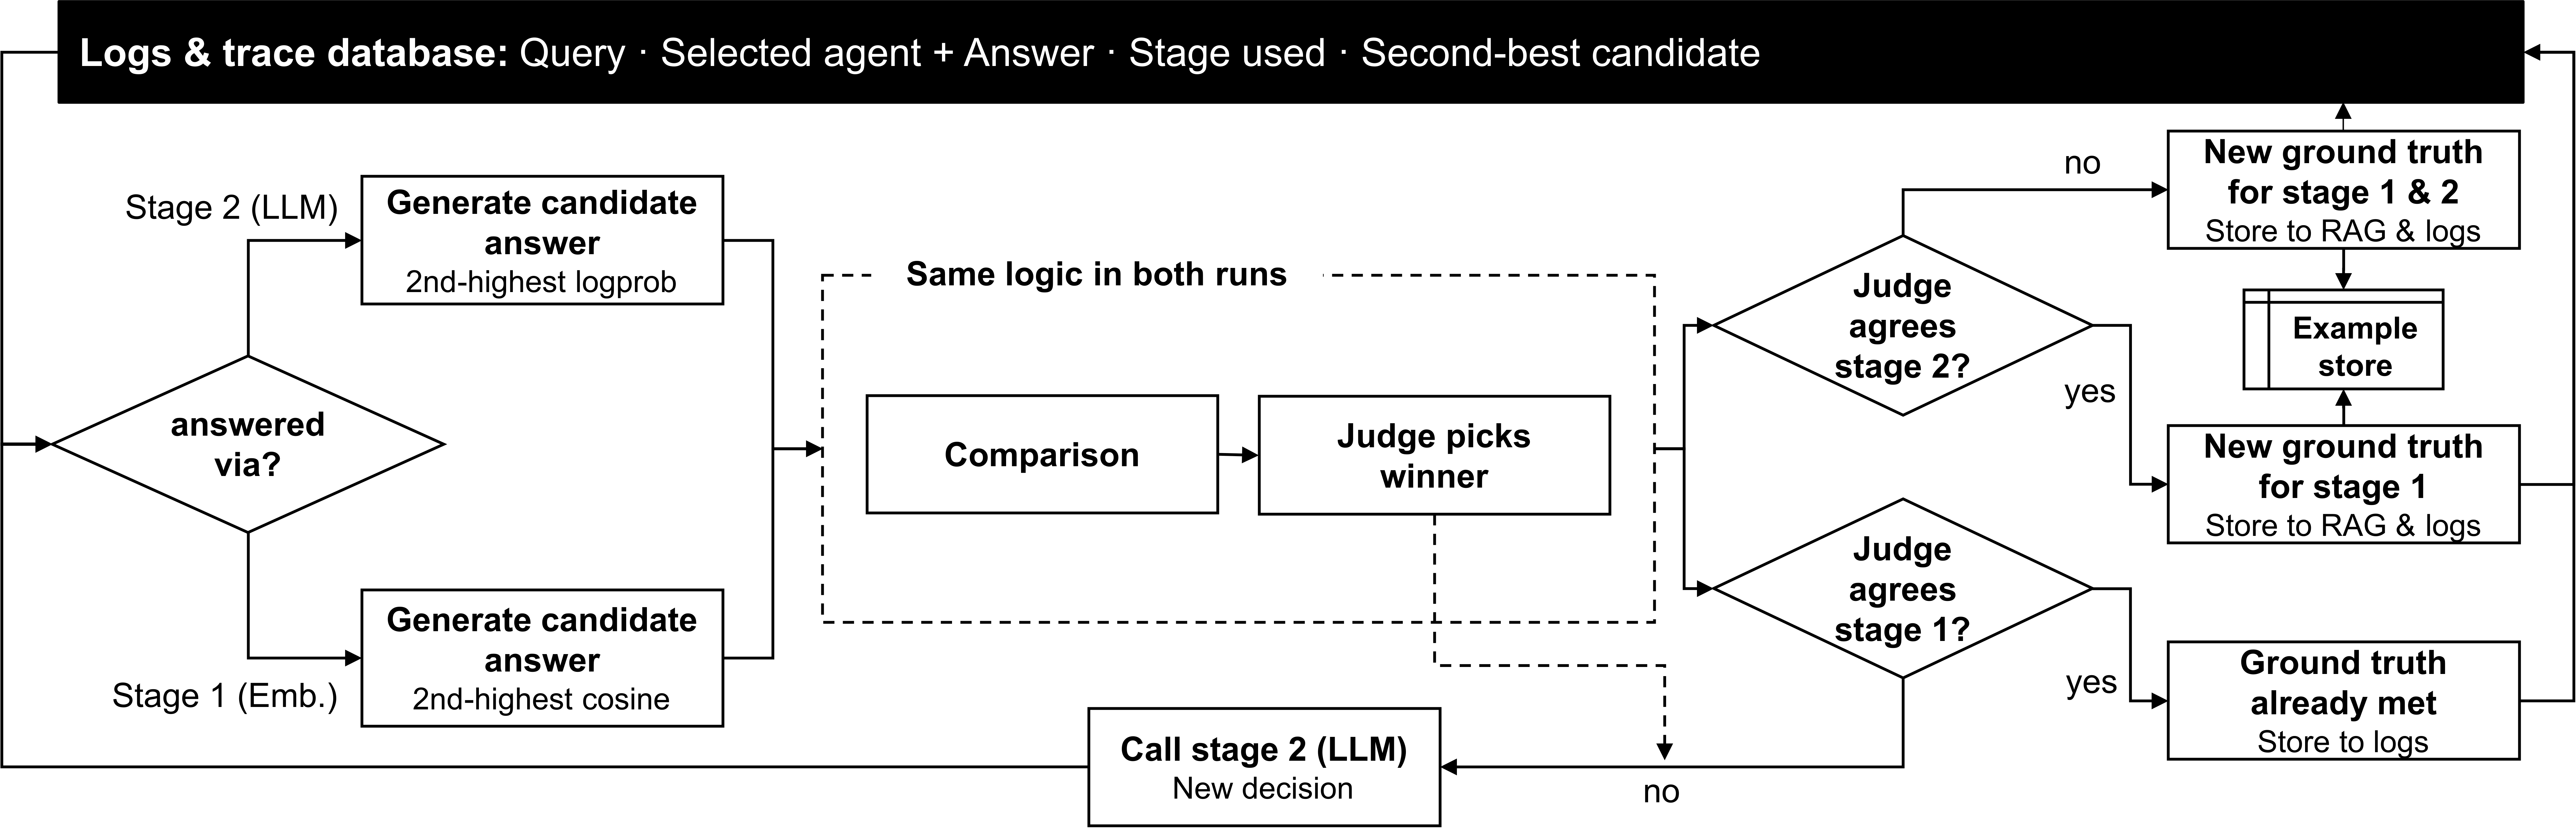
\includegraphics[keepaspectratio]{assets/pipeline/judge-process.png}}
\caption{Process Diagram of the Judge module with Stage 1 correction mechanism and storage of signals for the optimizer.}
\label{fig:judge-process}
\end{figure}


Within the judge module, several distinctions are made when a new query to be evaluated is consumed from the router's logs. First, a check is performed which Stage of the router performed the routing decision. If Stage 1 routed the query and the judge agrees, no correction is written, as Stage 1 is already correct. If Stage 1 routed the query and the judge disagrees, the query is escalated to Stage 2, which identifies its own top two candidates. Since these can differ from Stage 1's choices, Stage 1's original winner is carried into this second evaluation alongside the Stage 2 candidates, so the judge compares all three together rather than only the two Stage 2 proposed. This ensures that in ambiguous cases where Stage 1 and Stage 2 choose different agent pairs, the judge considers a broader scope of potential agents for the evaluation. If the query was initially already routed via Stage 2, this indicates that Stage 1 was too uncertain to decide at all, as no agent-specific threshold was met. In this case the judge evaluates Stage 2's decision directly and writes the query and the winning agent back to the example store of Stage 1.

In short, Stage 1 is corrected whenever it was wrong or too uncertain to decide, while the optimizer receives a signal whenever Stage 2 itself was judged incorrect. A novelty check blocks entries whose cosine similarity to an existing example exceeds 0.96, preventing redundant duplicates. Over time, this write-back extends the range of queries that Stage 1 resolves directly, which reduces the number of escalations to Stage 2 of the router and with that the cost and latency, while improving accuracy.

\authoredsubsection{Optimizer}{Gáspár}{Gáspár Harmati}\label{sec:optimizer}

\subsubsection{Role in the Pipeline}\label{sec:optimizer-role}

The optimizer runs last and closes the evaluation loop. The router routes live broker queries, the judge grades those decisions and records the correct answer together with its reasoning, and the optimizer learns a better routing prompt from that verdict file. It improves only Stage 2 of the router (\cref{sec:router-stage2}).

Rewriting that prompt by hand does not scale, and intuition about wording is unreliable, since semantically similar prompts can perform very differently on the same task \autocite{yang2023llmoptimizers}. Automatic prompt optimization treats prompt design instead as a heuristic search problem \autocite{cui2025aposurvey,ramnath2025aposurvey}. We adopted Optimization by PROmpting (OPRO), in which an optimizer LLM is shown past instructions with their scores and proposes a better one, so that the trajectory of scored attempts supplies the direction of improvement a gradient would otherwise give \autocite{yang2023llmoptimizers}. Gradient-based methods were unavailable, as they require model weights that our routing models, and more importantly Interhyp's, do not expose. Among the black-box alternatives, APE scores each candidate independently and keeps the best, without memory of what came before \autocite{zhou2023ape}. OPRO's memory of the whole trajectory suits our problem, where failures are spread across eight agent definitions at once.

\subsubsection{Implementation}\label{sec:optimizer-implementation}

The optimizer operates asynchronously on the judge's verdict file alone. It never runs the judge and never generates agent responses, it reruns only Stage 2. Each round follows four phases.

In proposal, an optimizer model (Gemini 3.1 Flash Lite) writes five candidate prompts at once, guided by a meta-prompt with four ingredients: the trajectory of every prompt tried so far with its score, ordered worst to best so the strongest sits last where the model attends most, per-agent exemplars of queries and their correct agents, six reserved for each of the eight agents and resampled every round to prevent fixation, the judge's explanations of past misroutes, and hard formatting rules that keep a candidate compatible with the router, namely the A to H letter mapping, the query placeholder, and a length ceiling. The exemplar count was itself tuned over several runs, since too few leave the rare agents unrepresented and too many crowd out the trajectory.

In measurement, each candidate is installed into Stage 2 and run over the training cases by a separate scoring model (GPT 5.4 nano). A different model is used following OPRO's separation of the optimizer LLM that writes candidates from the scorer LLM that evaluates them \autocite{yang2023llmoptimizers}. Prompt writing rewards a strong generative model, while scoring must expose token log probabilities to produce a graded distribution over the agents, which the optimizer's LLM does not expose. A candidate's score is the fraction of queries routed to the agent the judge selected. That target rather than the golden dataset label is used because the deployed system has no golden label, so optimizing toward one would optimize toward a signal absent at run time. Golden-label accuracy is computed in the same pass and reported alongside, but never influences the search.

In selection, every scored candidate is appended to the trajectory, and a new best is written to disk immediately. Selection uses the training score, since a held-out validation slice saturated to 1.000 in the first round on our skewed verdict files and stopped discriminating while still able to lock in a worse prompt. This follows the paper's own fallback, that where candidates overfit to a similar extent, the higher-training-accuracy solution still generalizes better \autocite{yang2023llmoptimizers}.

In iteration, the loop repeats until training accuracy reaches 100 percent, five consecutive rounds pass without gain, or a ten-round budget is exhausted. After two flat rounds, the mutation temperature rises briefly to encourage exploration.

Two deviations from standard OPRO are deliberate. We rewrite the entire prompt rather than an instruction snippet, and we add a natural-language feedback block, which OPRO names as future work and ProTeGi demonstrates in practice, propagating a criticism derived from errors back into the prompt \autocite{pryzant2023protegi,yang2023llmoptimizers}.

\subsubsection{Evolution, from DSPy to OPRO}\label{sec:optimizer-evolution}

The framework changed because our error distribution did not suit the alternative. DSPy compiles declarative language model calls into optimized pipelines \autocite{khattab2024dspy}, and its MIPROv2 optimizer runs a Bayesian search over instruction and demonstration combinations \autocite{opsahlong2024mipro}. Our proof of concept failed twice, instructively. The first run returned identical baseline and optimized accuracy because DSPy invoked the full router, and Stage 1 resolved most validation examples before they reached the LLM layer, leaving Stage 2 three queries to be judged on. The second failed on coverage: Bayesian search needs a signal that varies across the space it searches, and our misroutes were concentrated in four boundary pairs out of fifty-six possible confusions.

Given the full 548-example set, MIPROv2 did improve routing accuracy from 95.45 to 96.59 percent. OPRO reached 98.6 percent from a comparable baseline on the same data, because its meta-prompt carries judge-confirmed corrections, a contrastive signal aimed at the failures themselves rather than inferred from broad statistical sampling.

\subsubsection{The Optimization Dashboard}\label{sec:optimizer-dashboard}

The optimizer outputs its results in a console log, which is also saved on the system. We designed and built a dashboard that presents the same run as a single view (\cref{fig:optimization-dashboard}). It is a demonstration of the intended interface rather than a live component, since the live pipeline has a different dashboard more suited for everyday monitoring than for optimization setup (\cref{sec:evaluation-training-optimization}).

\begin{figure}
\centering
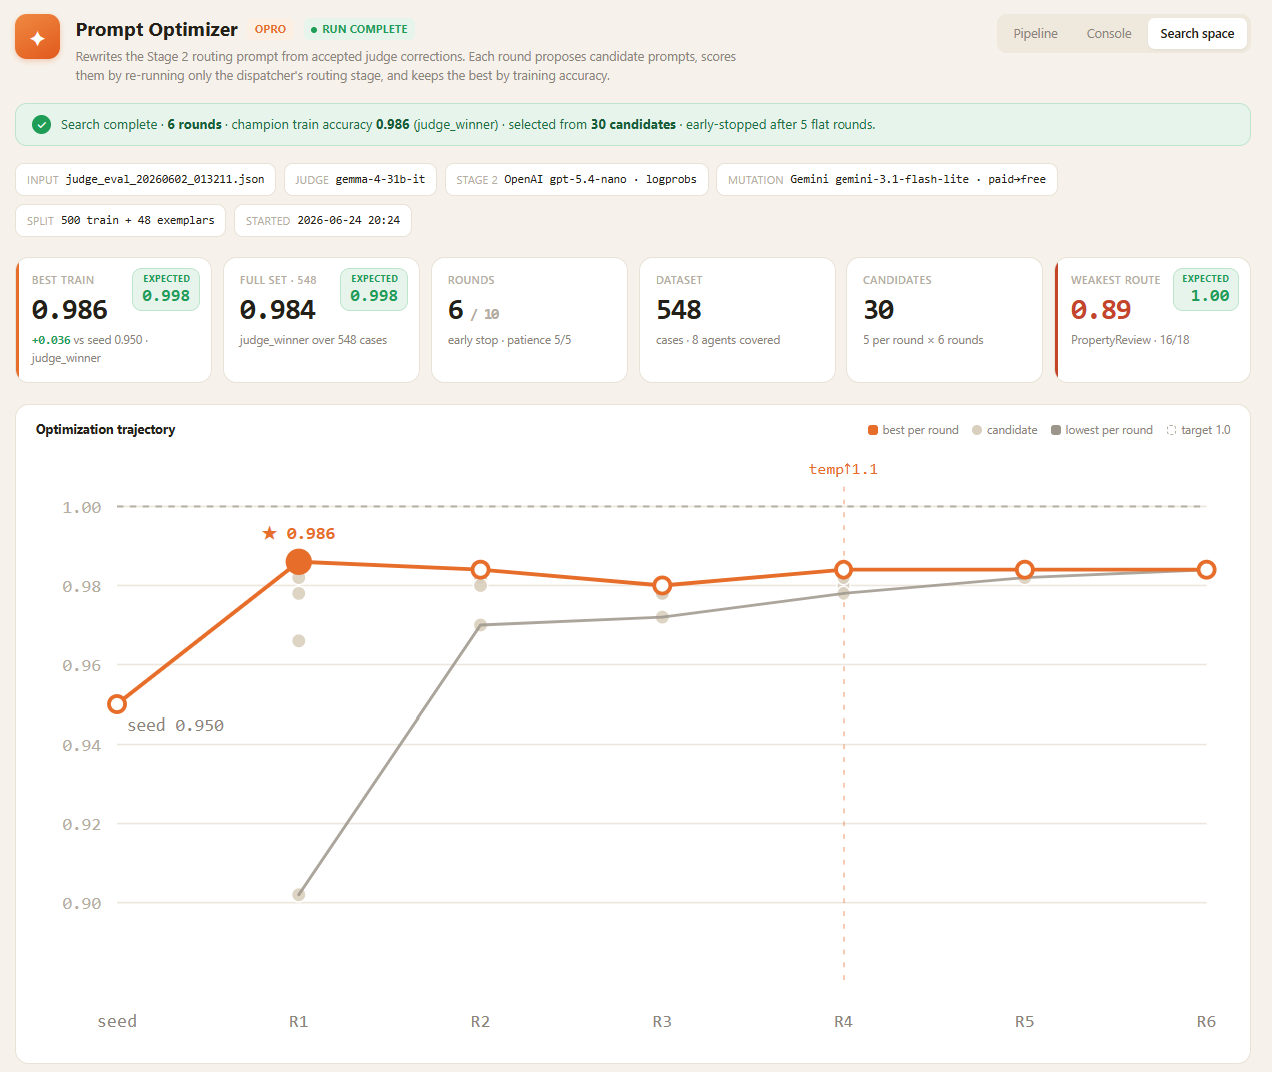
\includegraphics[width=1\linewidth,height=\textheight,keepaspectratio]{assets/pipeline/optimization-dashboard.png}
\caption{Optimization dashboard for the run of 24 June 2026 (development dashboard).}\label{fig:optimization-dashboard}
\end{figure}

\subsubsection{Evaluation}\label{sec:optimizer-evaluation}

The run in \cref{fig:optimization-dashboard} was chosen deliberately, as it is one of the weakest runs the optimizer produced, on the hardest data we have, a 548-case sample of the third-iteration golden dataset (\cref{sec:dataset-stages}).

The seed prompt was already written by us to be a good example of a well-written routing prompt, and it scored 0.950. The champion appeared in round 1 at 0.986 and was never beaten: rounds 2 to 6 returned 0.984, 0.980, 0.984, 0.984, and 0.984, and the run stopped early after five flat rounds. On the headline metric, therefore, five of six rounds bought nothing.

Reading only the best column misses what the run demonstrates. The floor rose while the ceiling stood still. In round 1 the five candidates spanned 0.902 to 0.986, a spread of more than eight points, and by round 6 all five scored 0.984 and the spread had closed entirely (\cref{fig:optimization-dashboard}). The mutator was not producing a better champion, but it had stopped producing bad prompts, which is the trajectory doing its work: shown every scored attempt in ascending order, the model learned what a competent routing prompt looks like even after it had stopped finding a superior one. This is the mechanism the natural-language gradient is supposed to supply, visible in a run where the headline metric shows nothing.

The run also exercises the plateau-escape rule. After rounds 2 and 3 passed without improvement, round 4 was mutated at a temperature of 1.1 instead of 0.8 and then reverted. It did not break the plateau, which is the honest outcome to report: the escape is one bounded attempt at divergence, not a guarantee, and patience still ended the run as designed.

The most interesting result is the divergence between the two labels. Measured against the judge, the champion routes 0.984 of the full set correctly. Measured against the golden dataset labels, it routes 0.998, a single misroute in 548 cases (\cref{tbl:optimizer-champion}).

\begin{longtable}[]{@{}
  >{\raggedright\arraybackslash}p{(\linewidth - 6\tabcolsep) * \real{0.3400}}
  >{\raggedright\arraybackslash}p{(\linewidth - 6\tabcolsep) * \real{0.2000}}
  >{\raggedright\arraybackslash}p{(\linewidth - 6\tabcolsep) * \real{0.2100}}
  >{\raggedright\arraybackslash}p{(\linewidth - 6\tabcolsep) * \real{0.1500}}@{}}
\caption{Champion accuracy by agent under both labelings. Case counts differ because the judge and the golden dataset assign some queries to different agents.}\label{tbl:optimizer-champion}\tabularnewline
\toprule\noalign{}
\begin{minipage}[b]{\linewidth}\raggedright
Agent
\end{minipage} & \begin{minipage}[b]{\linewidth}\raggedright
By judge label
\end{minipage} & \begin{minipage}[b]{\linewidth}\raggedright
By golden label
\end{minipage} & \begin{minipage}[b]{\linewidth}\raggedright
Cases
\end{minipage} \\
\midrule\noalign{}
\endfirsthead
\toprule\noalign{}
\begin{minipage}[b]{\linewidth}\raggedright
Agent
\end{minipage} & \begin{minipage}[b]{\linewidth}\raggedright
By judge label
\end{minipage} & \begin{minipage}[b]{\linewidth}\raggedright
By golden label
\end{minipage} & \begin{minipage}[b]{\linewidth}\raggedright
Cases
\end{minipage} \\
\midrule\noalign{}
\endhead
\bottomrule\noalign{}
\endlastfoot
CoachAgent & 1.00 & 1.00 & 11 / 12 \\
EmailAgent & 0.98 & 1.00 & 266 / 264 \\
ExposeAgent & 1.00 & 1.00 & 34 / 35 \\
GeneralPurposeAgent & 0.98 & 0.99 & 114 / 114 \\
MarketInfoAgent & 0.98 & 1.00 & 52 / 51 \\
OfferAgent & 1.00 & 1.00 & 39 / 41 \\
PlatformSupportAgent & 1.00 & 1.00 & 14 / 15 \\
PropertyReviewAgent & 0.89 & 1.00 & 18 / 16 \\
Full set & 0.984 & 0.998 & 548 \\
\end{longtable}

The optimizer therefore outperforms the examiner it was trained against, and the reason is structural rather than accidental. A judge's errors on individual cases are largely inconsistent, since the same query judged twice can fall either way, whereas the distinctions that actually separate two agents recur across many cases. A prompt is a single instruction of at most a few thousand characters, scored on hundreds of cases at once, so it has no capacity to encode a case-by-case correction: it can only capture what generalizes. Idiosyncratic judge noise is not learnable at that granularity and is left behind, while the systematic signal survives. The trajectory reinforces this, because a candidate that happened to fit a few noisy labels does not score consistently well across rounds and is not carried forward.

The weakest route under the judge's labeling is PropertyReviewAgent at 0.89, which is the same boundary the router struggles with (\cref{sec:router}) and the one the golden labeling shows as clean, another sign that the residual disagreement is the judge's rather than the prompt's.



\clearpage
\suppressfloats[t]
\authoredsection{Chatbot Showcase Application}{Julius}{Julius Bethge}\label{sec:chatbot-application}

\subsection{Purpose and Design Rationale}\label{sec:application-purpose}

The pipeline components presented in the preceding chapter were integrated into a fully functioning showcase application. It provides one environment in which a user query can be routed, its trace inspected and evaluated, and resulting examples used for training or prompt optimization. The application was used by the project team, our Interhyp partners from the Data Science team, and is available to the supervisors from the LMU. It supported the development and evaluation of the pipeline as well as its demonstration within a fully functioning application. It is not an advisor-facing production system, a replacement for Robin, or a system already integrated into Interhyp's operational environment.

The application provided the project team and Interhyp with a shared environment for inspecting pipeline behavior, comparing configurations, and discussing potential integration. It can therefore be interpreted as a potential boundary object between technical development and stakeholder evaluation.\autocite{star-griesemer} This describes its intended role rather than an empirically tested organizational effect.

Validated approaches from the experimental \texttt{pipeline} repository were reimplemented in the maintainable \texttt{chatbot} showcase application.\autocite{amershi-ml-se}

Early integrations connected Python components through subprocesses and local files. Although functional, they lacked persistent shared state, coordination of long-running jobs, live progress, and lineage from a query through routing, answering, judging, and optimization. This confirmed that model code forms only one part of a complete machine-learning system.\autocite{sculley-technical-debt} We therefore retained a modular Python worker and added Convex for orchestration and persistence and React for presentation, preserving Python library access and replaceable providers while accelerating integration and deployment.

\subsection{Modular Architecture and Technology Rationale}\label{sec:application-architecture}

\subsubsection{Overall Architecture and Execution Flow}\label{sec:application-flow}

The architecture consists of a React frontend, Convex backend, and Python worker. Convex forms the shared state and orchestration layer. The frontend never calls the worker directly. This reflects the idea of a layered modular architecture in which components communicate through defined interfaces and can evolve or be recombined.\autocite{yoo-digital-innovation} Its specific realization with React, Convex, and Python is a project decision.

\begin{figure}
\centering
\pandocbounded{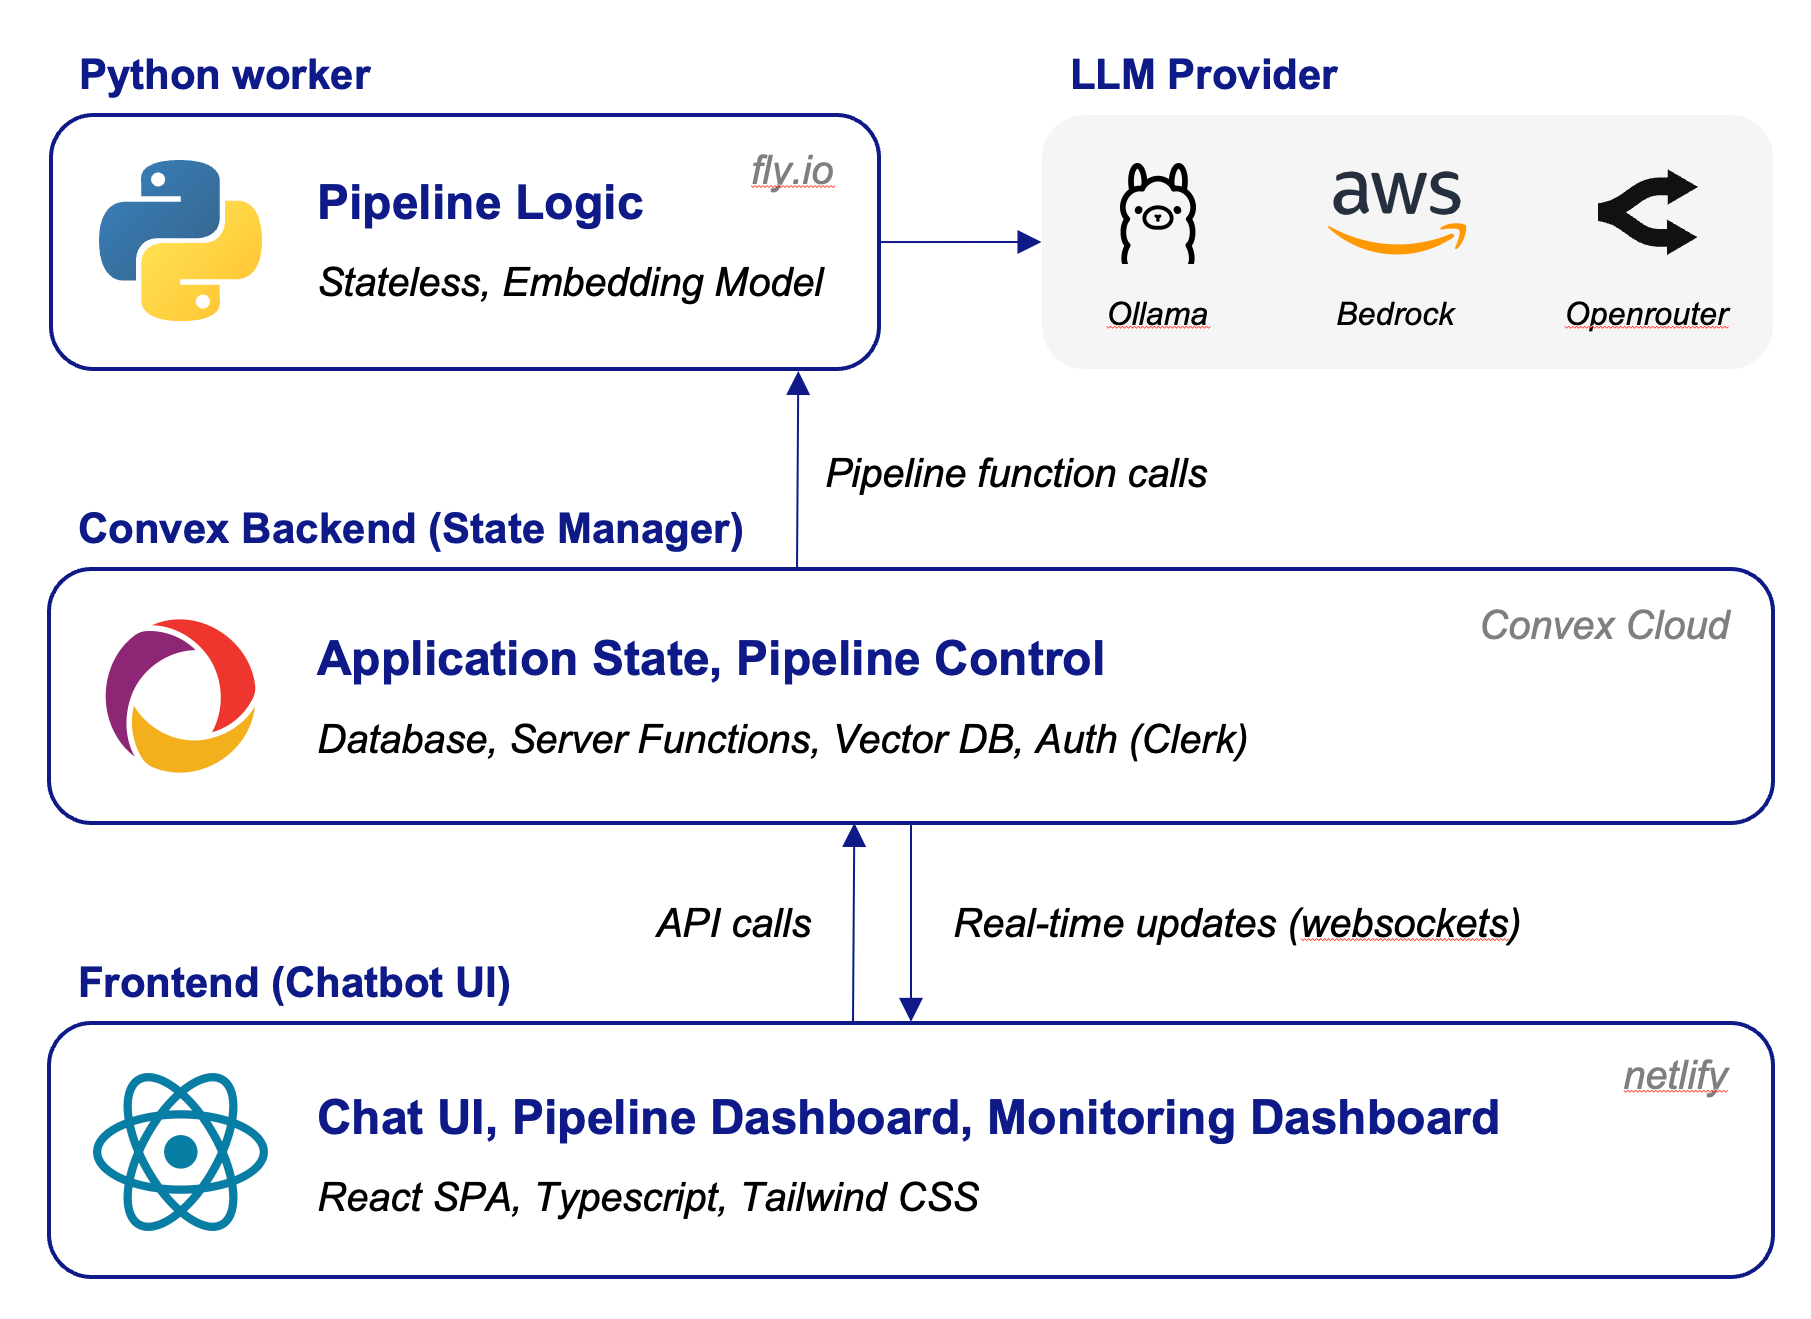
\includegraphics[keepaspectratio]{assets/application/architecture.png}}
\caption{Technical stack connecting the React frontend, Convex state layer, Python pipeline worker, and model providers}
\label{fig:application-architecture}
\end{figure}

Each operation is represented as a Convex job that the worker claims and updates with step statuses, inputs, outputs, errors, and timestamps before storing the resulting trace or run. Frontend subscriptions expose progress and preserve completed results across reloads, linking the same execution to the chatbot, pipeline, judge, training, and optimization views. Job states distinguish queued, running, successful, and failed executions, while step states also represent skipped conditional branches. The same protocol therefore supports interactive chat and longer batch or optimization runs without equating completion of a browser request with completion of the underlying computation.

\subsubsection{Python Worker}\label{sec:python-worker}

Python was retained because its machine-learning ecosystem provides the libraries and integrations required for embedding, model access, evaluation, and optimization.\autocite{raschka-python-ml} The worker owns all pipeline logic, including Stage 1 and Stage 2 routing, agent generation, judging, batch processing, index construction, and OPRO; Convex only schedules these operations and persists their state.

Provider interfaces decouple routing, completion, judging, optimization, and embedding from individual model services. Configuration selects execution mode, model identifiers, endpoints, timeouts, and credentials without changing the job protocol, trace model, or pipeline interfaces. Convex and React therefore form the showcase environment, while the worker remains reusable and could be adapted to Interhyp-approved endpoints. Such an integration was not performed.

This ownership boundary keeps embedding, routing, judging, and optimization decisions out of the backend and frontend. Either application layer could consequently be replaced without reconstructing pipeline rules.

\subsubsection{LLM and Embedding Provider Layer}\label{sec:provider-layer}

Stage 1 executes \texttt{multilingual-e5-large} inside the worker through FastEmbed's ONNX-based runtime and quantized weights.\autocite{fastembed-docs} The same setup is used locally and in the hosted application, avoiding changes in embedding behavior during integration. Computational efficiency also supported worker-local execution,\autocite{schwartz-green-ai} although a production deployment should compare it with a central embedding service when scaling workers.

Stage 2 requires token log probabilities, which OpenRouter exposes through \texttt{logprobs} and \texttt{top\_logprobs}.\autocite{openrouter-parameters} It therefore serves Stage 2 in the deployed configuration, while AWS Bedrock handles agent responses, judging, and OPRO using the available credits. Ollama remains the free local option but was too slow for some repeated and batch workflows. Because the hosted showcase cannot depend on a developer's computer, hosted mode uses OpenRouter and Bedrock, whereas local mode uses Ollama. The shared interfaces allow either configuration to be replaced with Interhyp-approved models.

\subsubsection{Convex Backend}\label{sec:convex-backend}

Convex forms the orchestration and state layer, storing jobs and steps, traces, prompt versions, vector entries, evaluation and training runs, and optimization history. Reactive queries expose worker progress without a separate WebSocket service or frontend polling,\autocite{convex-realtime} while schema-defined vector indexes support Stage 1 similarity search and retain links to source traces.\autocite{convex-vector-search} Generated TypeScript definitions connect backend functions with frontend queries and mutations.

Persistence makes lineage explicit through immutable prompt versions, a separately identified deployed version, run configurations, dataset snapshots, and traces linking queries to routing scores, agents, answers, timings, and judge outcomes. This extends model-management principles for retaining parameters, metrics, datasets, and historical changes.\autocite{vartak-modeldb} Reproducibility also requires accessible data, code, procedures, and execution conditions.\autocite{pineau-reproducibility} Storage alone cannot reproduce a result, but snapshots prevent later prompt or dataset changes from altering the basis of earlier runs and keep comparisons tied to identifiable conditions.

\subsubsection{React Frontend}\label{sec:react-frontend}

The React single-page frontend uses Vite, TypeScript, and Tailwind CSS to start workflows through Convex, subscribe to their state, and render live and completed executions across the chat, pipeline, evaluation, training, and optimization views. Shared components provide consistent statuses, selectors, scores, controls, and detail panels. Because Convex subscriptions expose worker updates as application state, the same components can display pending and completed executions without a second real-time channel. Public indexing and server rendering were unnecessary for the internal demonstrator.

\subsubsection{Authentication and Deployment}\label{sec:application-deployment}

Frontend and worker access follow separate authorization paths. Users authenticate through Clerk and Convex email and domain allowlists, whereas the Python worker supplies a shared token accepted only by worker-facing functions. A frontend session therefore cannot invoke worker operations, and the worker token grants no frontend access.

Netlify serves the React build, Convex Cloud hosts state, and Fly.io runs the containerized worker, with a Fly volume retaining the FastEmbed cache. Moving the frontend from Vercel to Netlify avoided a projected USD 300 cost, while Ollama remained available only for local development. These boundaries were sufficient for the controlled showcase; production integration would require Interhyp to evaluate service identity and secret management.

\subsection{Application Workflows and User Interface}\label{sec:application-workflows}

The interface supports individual chatbot execution, pipeline inspection, and evaluation, training, and optimization. Visible status, consistent controls, and inspectable results reflect Nielsen's usability principles.\autocite{nielsen-usability}

\subsubsection{Chatbot Interface}\label{sec:chatbot-interface}

Submitting a request creates a chat job whose routing summary and message area update during Stage 1, possible Stage 2 escalation, and agent generation. The completed view shows the answer, selected agent, routing stage, leading scores or probabilities, threshold, timings, and available vector or prompt references. Previous traces can be restored without another model call, connecting user-facing answers with their technical evidence.

Interactions are intentionally single-turn, limiting conversational state as a confounding factor and producing a stable evaluation unit containing the query, decision, answer, configuration, and timings. Each completed trace can be opened in the pipeline view or submitted to the judge.

\begin{figure}
\centering
\pandocbounded{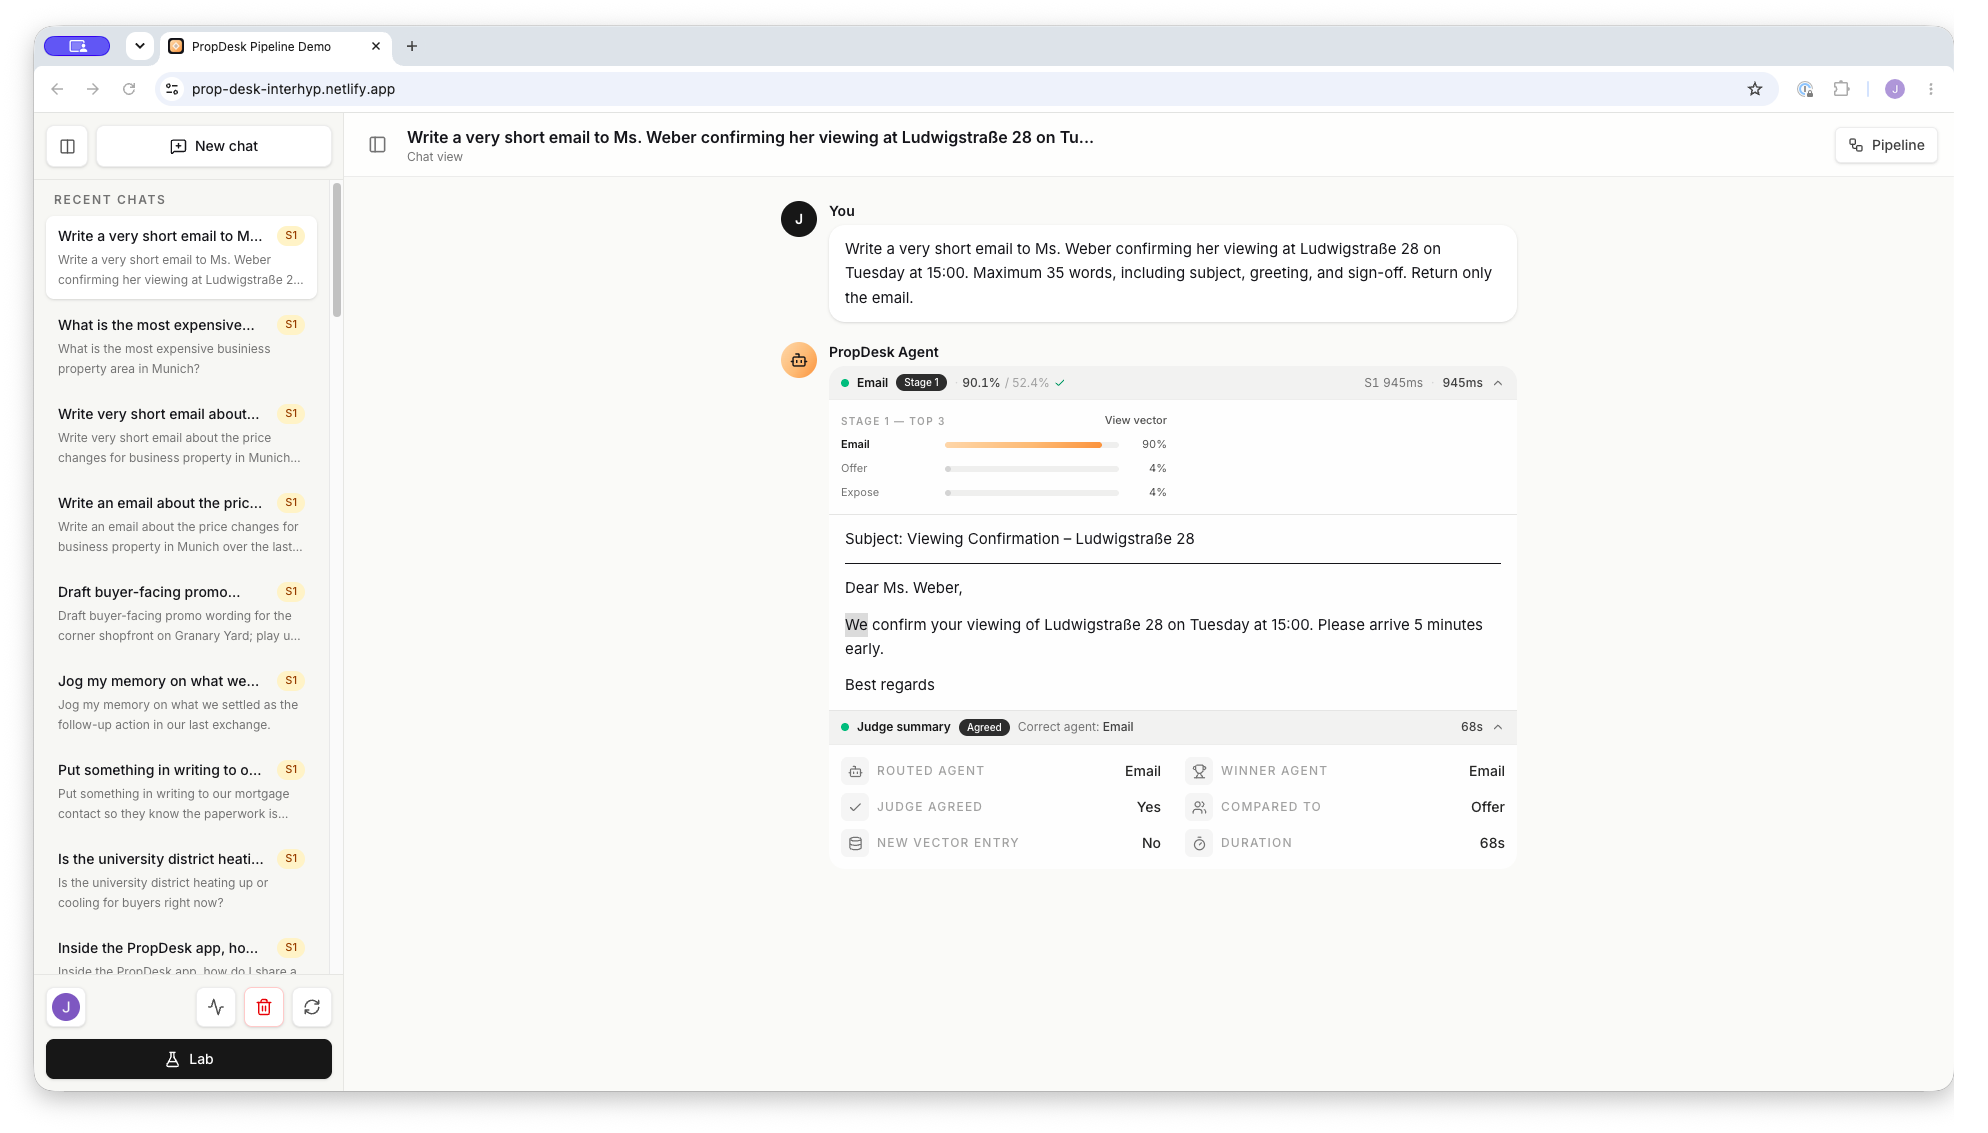
\includegraphics[keepaspectratio]{assets/application/chatbot-interface.png}}
\caption{Completed chatbot interaction with routing scores, trace history, and judge summary}
\label{fig:chatbot-interface}
\end{figure}

\subsubsection{Pipeline View}\label{sec:pipeline-view}

The pipeline view presents Router and judge execution as connected graphs. Nodes represent major steps and edges show their order and conditional paths. Pending, running, successful, skipped, and failed states change with the worker records. Stage 1 success follows a different visible path from Stage 2 escalation, and the judge pipeline becomes available for completed traces.

\begin{figure}
\centering
\pandocbounded{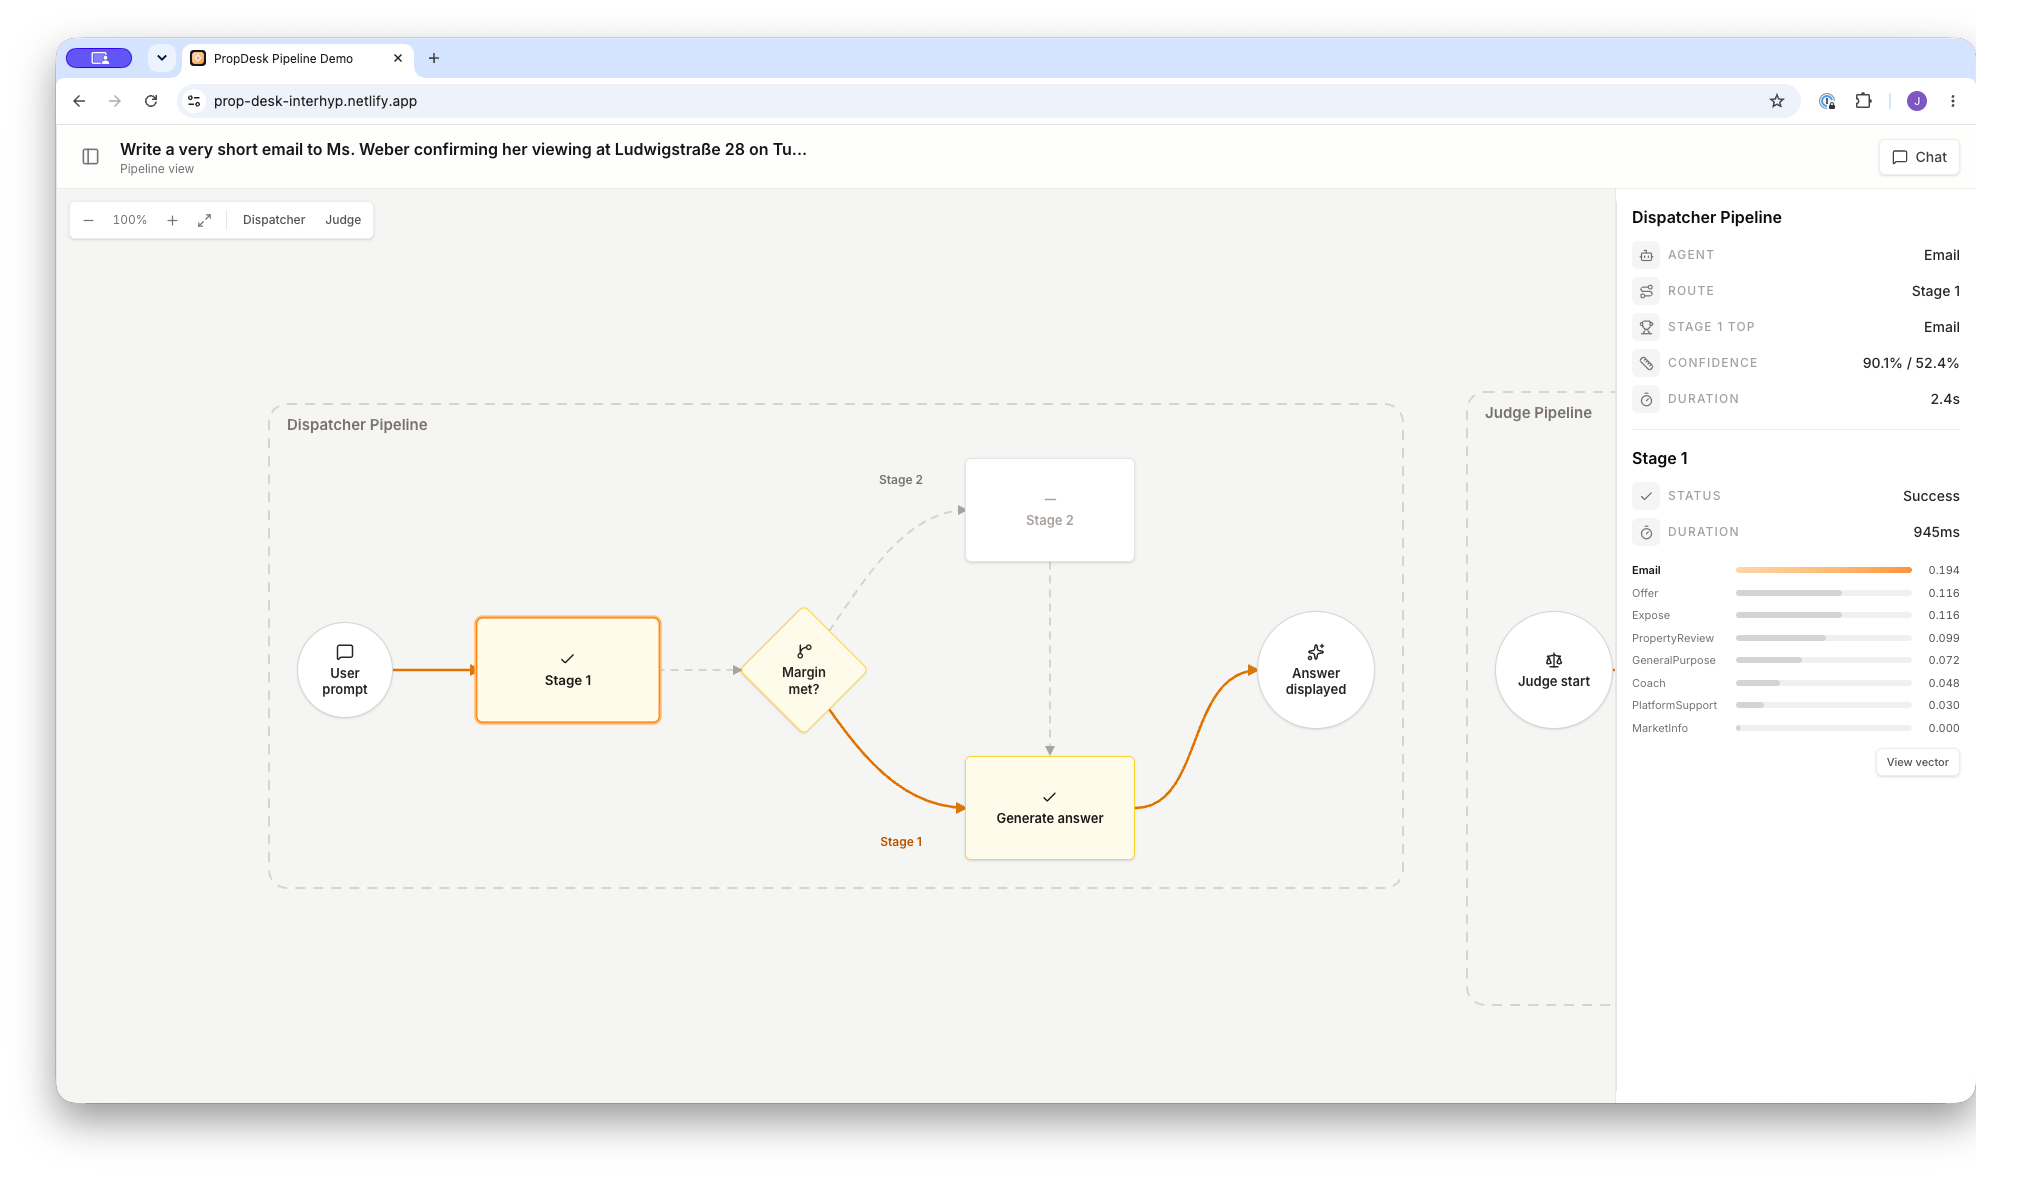
\includegraphics[keepaspectratio]{assets/application/router-pipeline.png}}
\caption{Router pipeline with the successful Stage 1 route and node inspector}
\label{fig:application-router-pipeline}
\end{figure}

Selecting a node opens an inspector with status, duration, inputs, outputs, scores, prompt or vector references, and stored payloads. This design applies Shneiderman's principle of providing an overview before details on demand.\autocite{shneiderman-eyes} It helps users understand an answer, locate unexpected execution and connect outcomes with intermediate evidence.

Conditional branches remain visible even when they are not executed, with their status distinguishing a skipped step from a failed one. This prevents a shortened Stage 1 path from appearing incomplete and makes Stage 2 escalation explicit. Router and judge diagrams share the same interaction pattern, so users can move from a high-level outcome to the evidence stored for a particular step without learning a separate inspection mechanism.

\begin{figure}
\centering
\pandocbounded{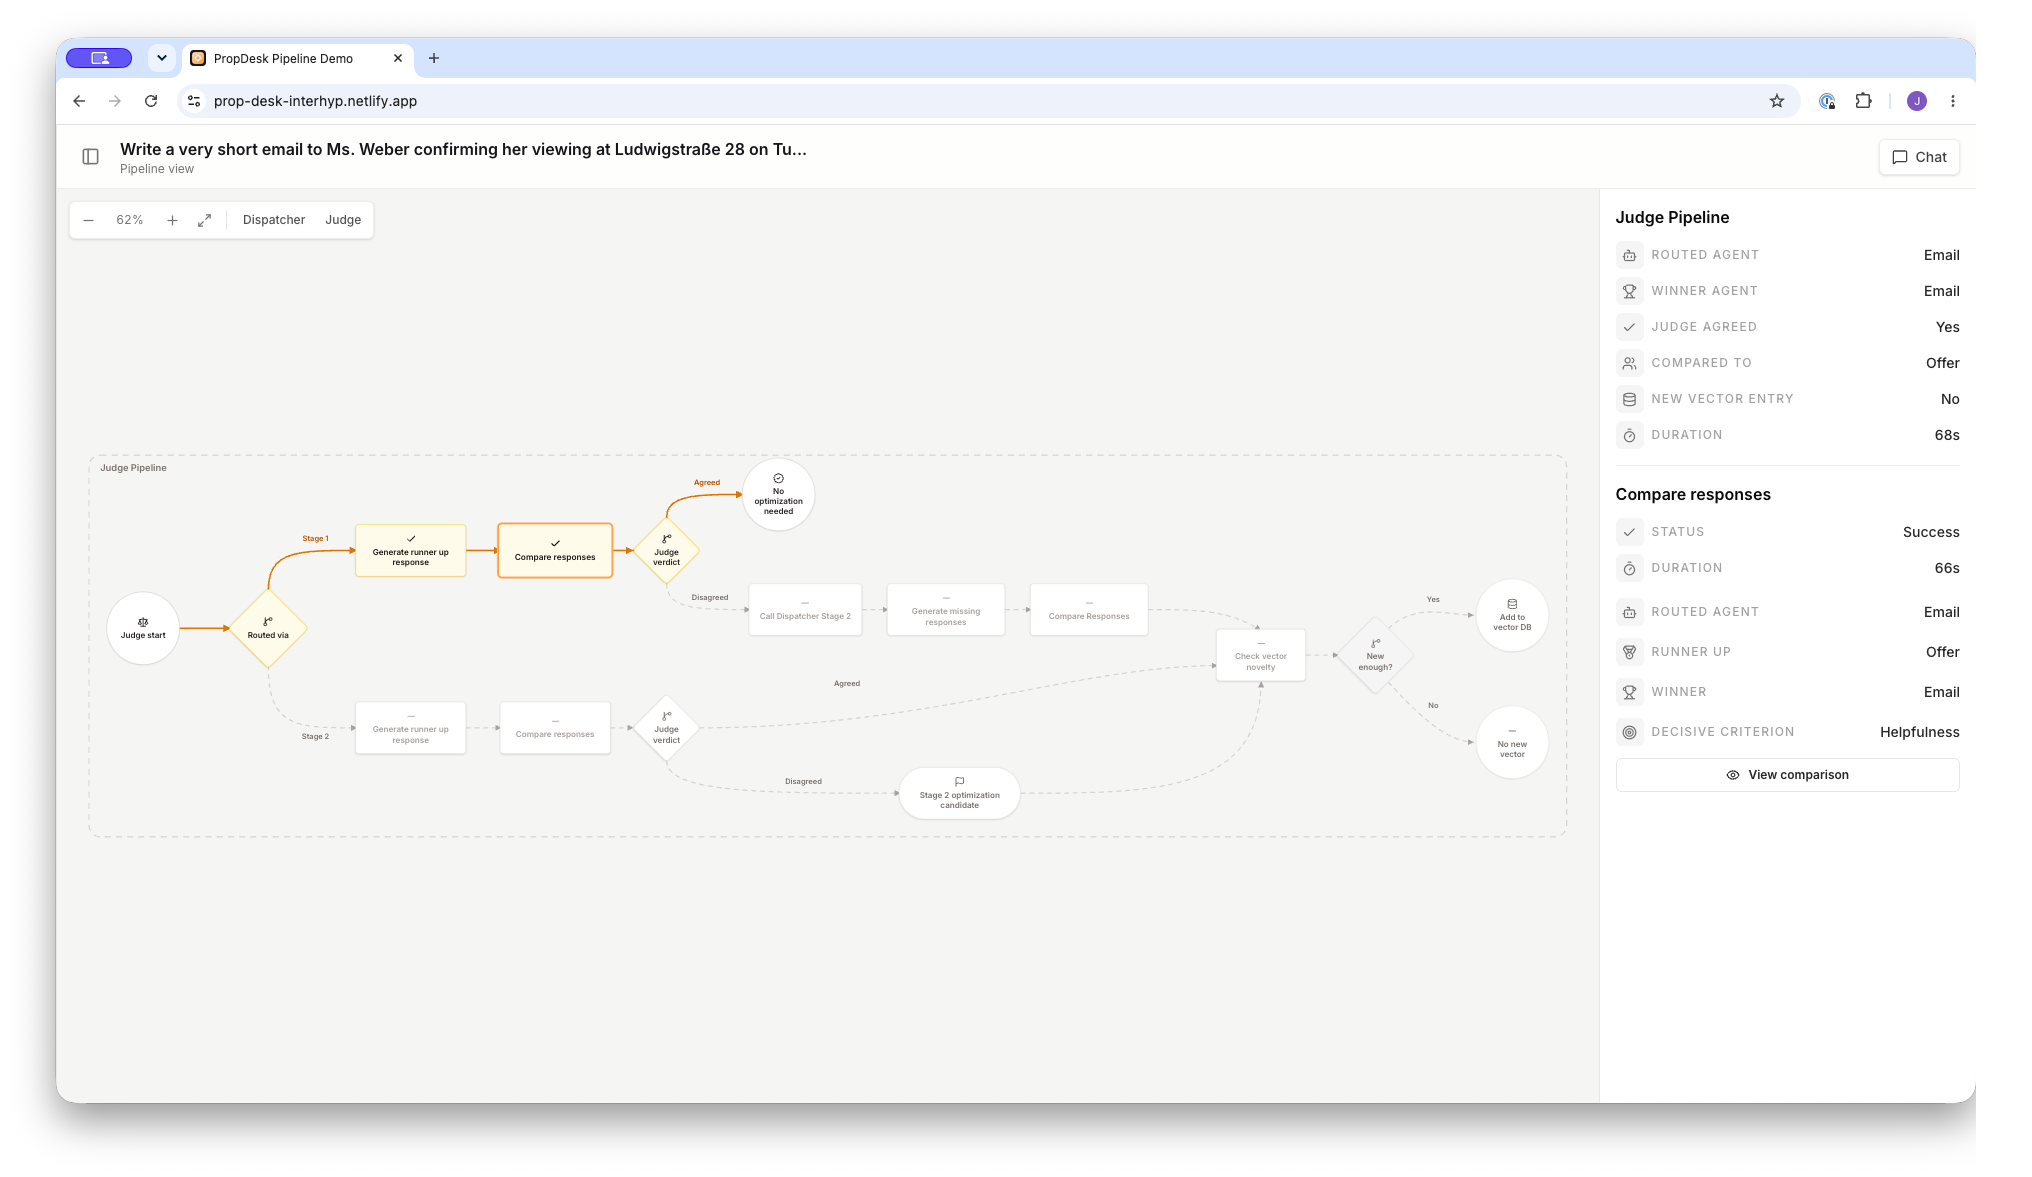
\includegraphics[keepaspectratio]{assets/application/judge-pipeline.png}}
\caption{Judge pipeline with the response-comparison step selected in the node inspector}
\label{fig:application-judge-pipeline}
\end{figure}

\subsubsection{Evaluation, Training and Optimization}\label{sec:evaluation-training-optimization}

The evaluation view runs a selected prompt version against the fixed evaluation dataset. Progress and individual outcomes remain visible during execution. Completed runs summarize accuracy, Stage 1 usage, latency, avoided LLM calls, misroutes, and per-agent results. Historical runs can be selected or compared while their prompt versions and configuration snapshots remain visible. A candidate can therefore be assessed under identifiable conditions before deployment.

\begin{figure}
\centering
\pandocbounded{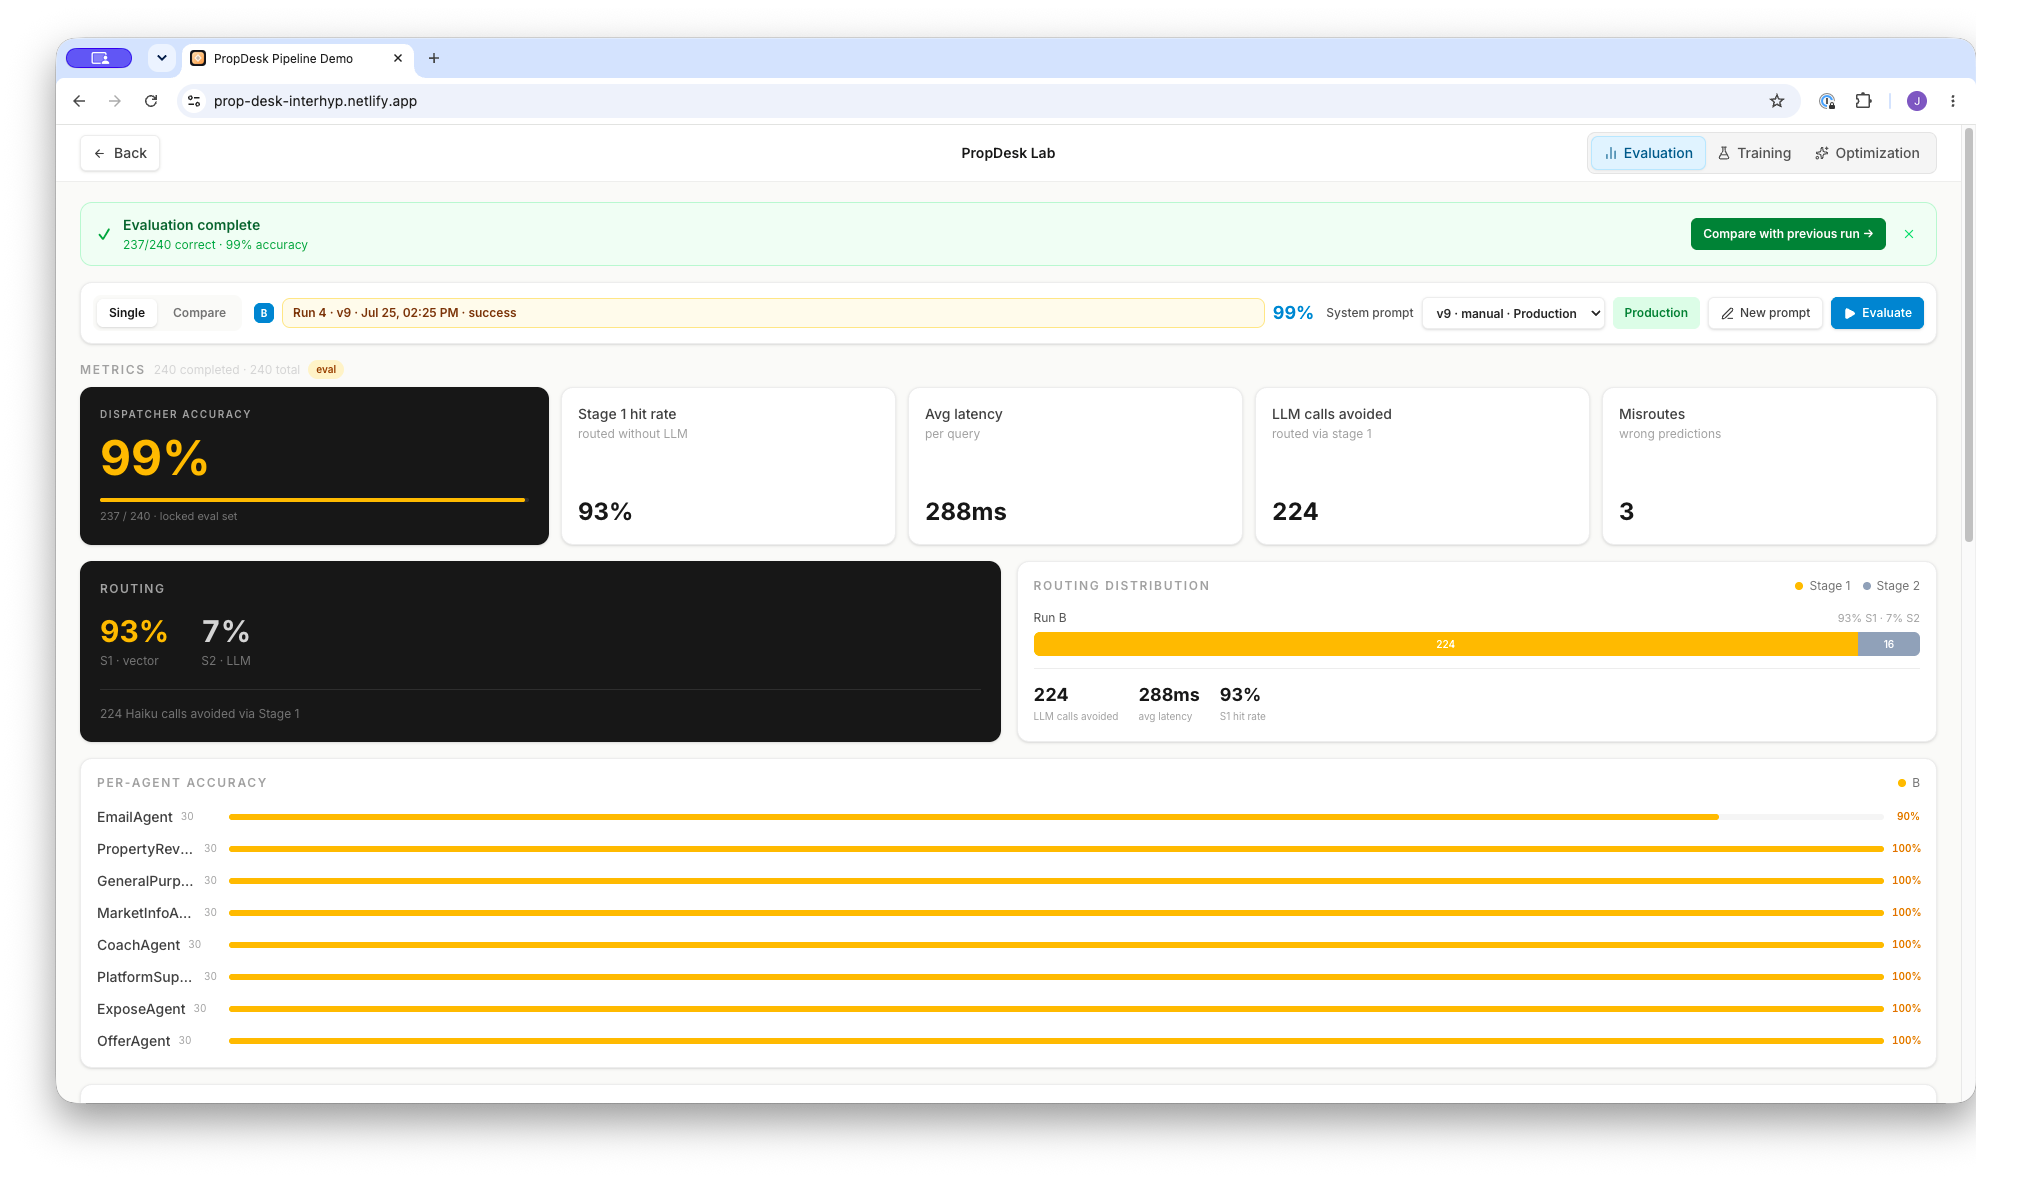
\includegraphics[keepaspectratio]{assets/application/evaluation-run.png}}
\caption{Completed evaluation run with routing, latency, and per-agent results}
\label{fig:application-evaluation}
\end{figure}

Training remains separate. Users upload labelled examples, and the application validates them and removes overlaps with the evaluation set. The resulting batch executes Router and judge workflows and records suitable Stage 1 corrections. A separate index-building job creates vector entries and threshold configuration while exposing its steps. This prevents evaluation examples from silently becoming training data.

\begin{figure}
\centering
\pandocbounded{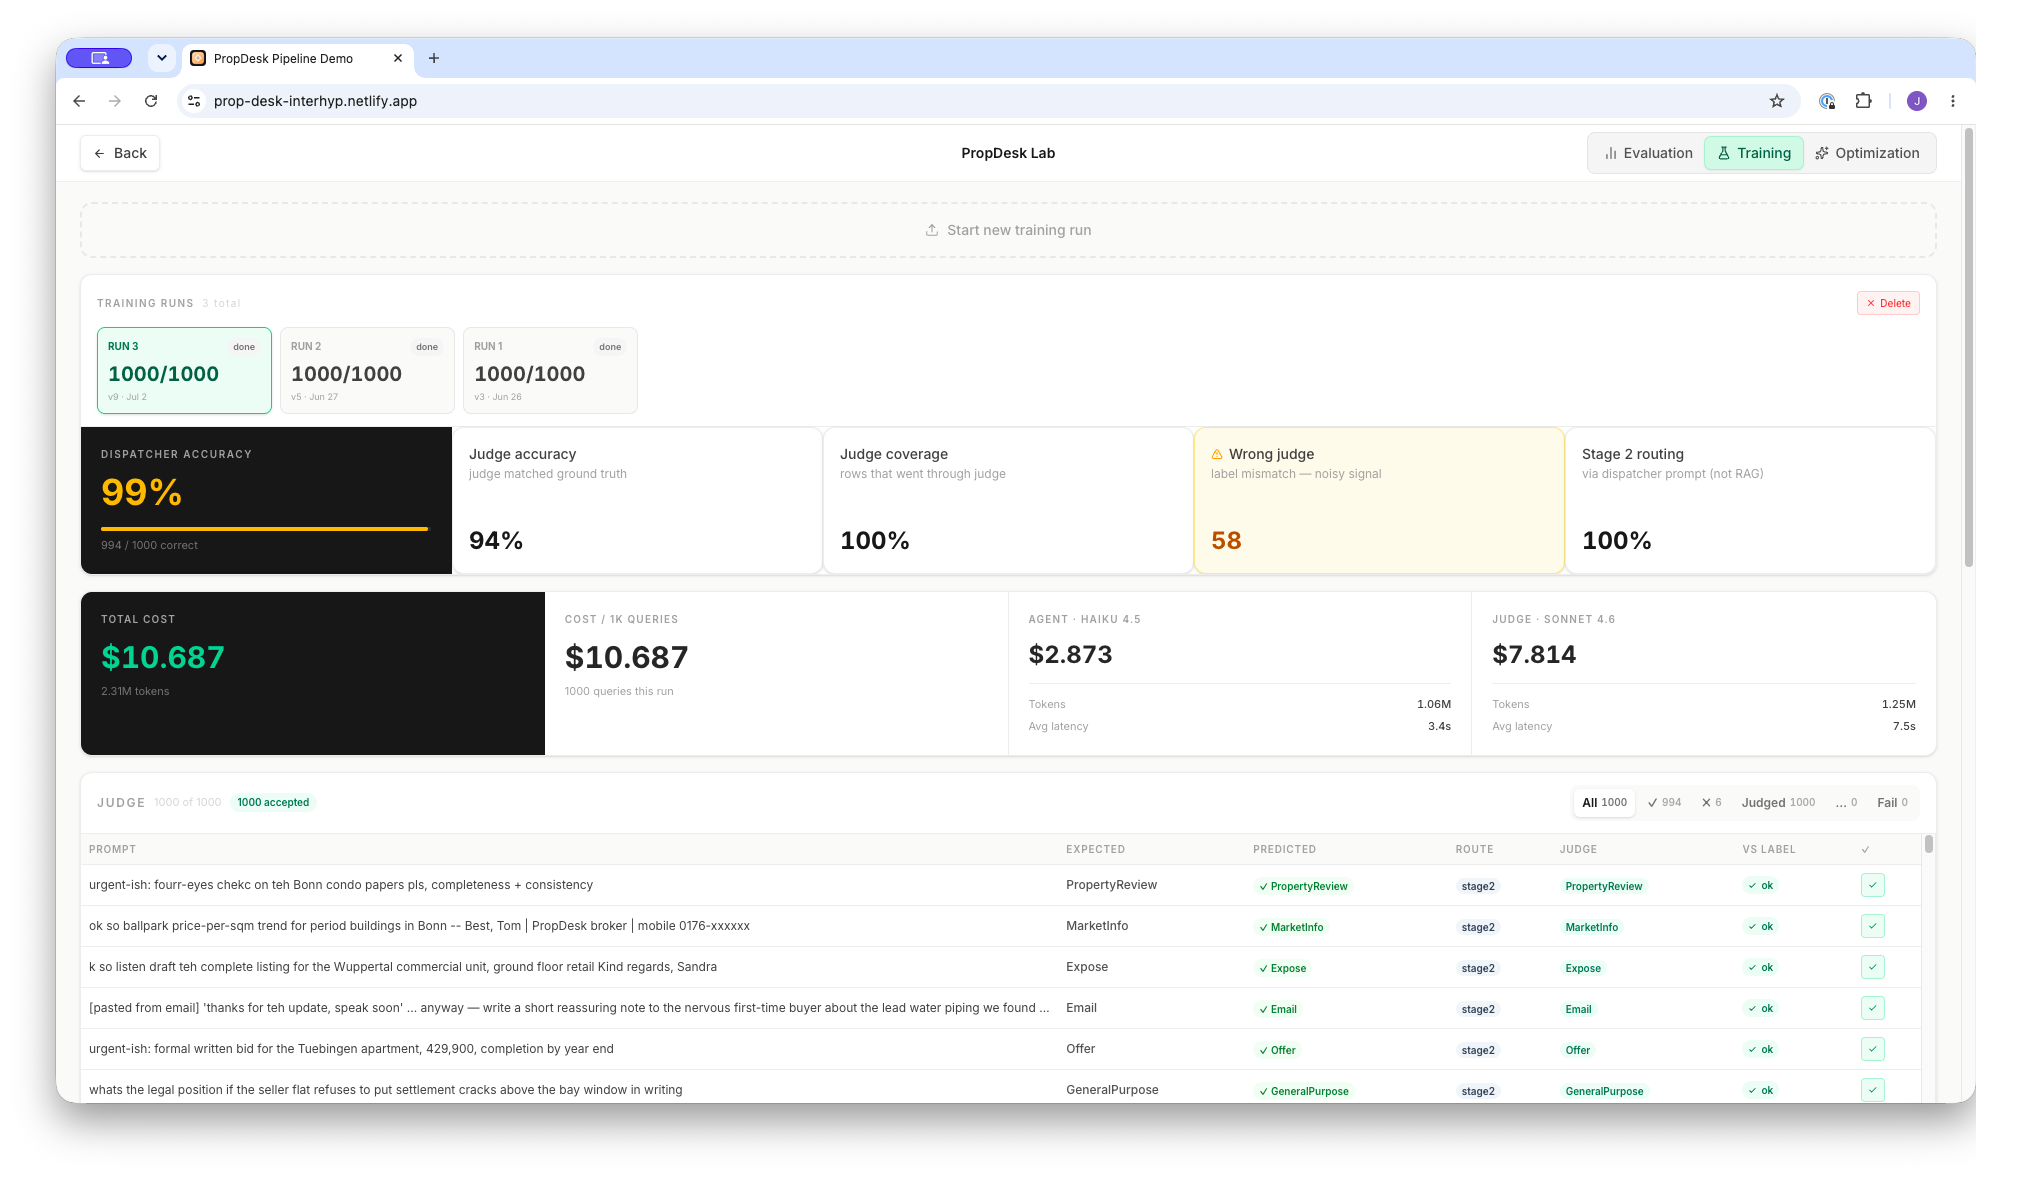
\includegraphics[keepaspectratio]{assets/application/training-run.png}}
\caption{Completed training run with routing, judge, cost, and trace-level results}
\label{fig:application-training}
\end{figure}

The optimization view applies OPRO to completed training data. Users follow rounds, candidate scores, and the optimization trajectory and can compare candidate prompts with the base prompt. Selecting a candidate creates a new prompt version. After evaluation, a version can be deployed without overwriting its predecessors.

\begin{figure}
\centering
\pandocbounded{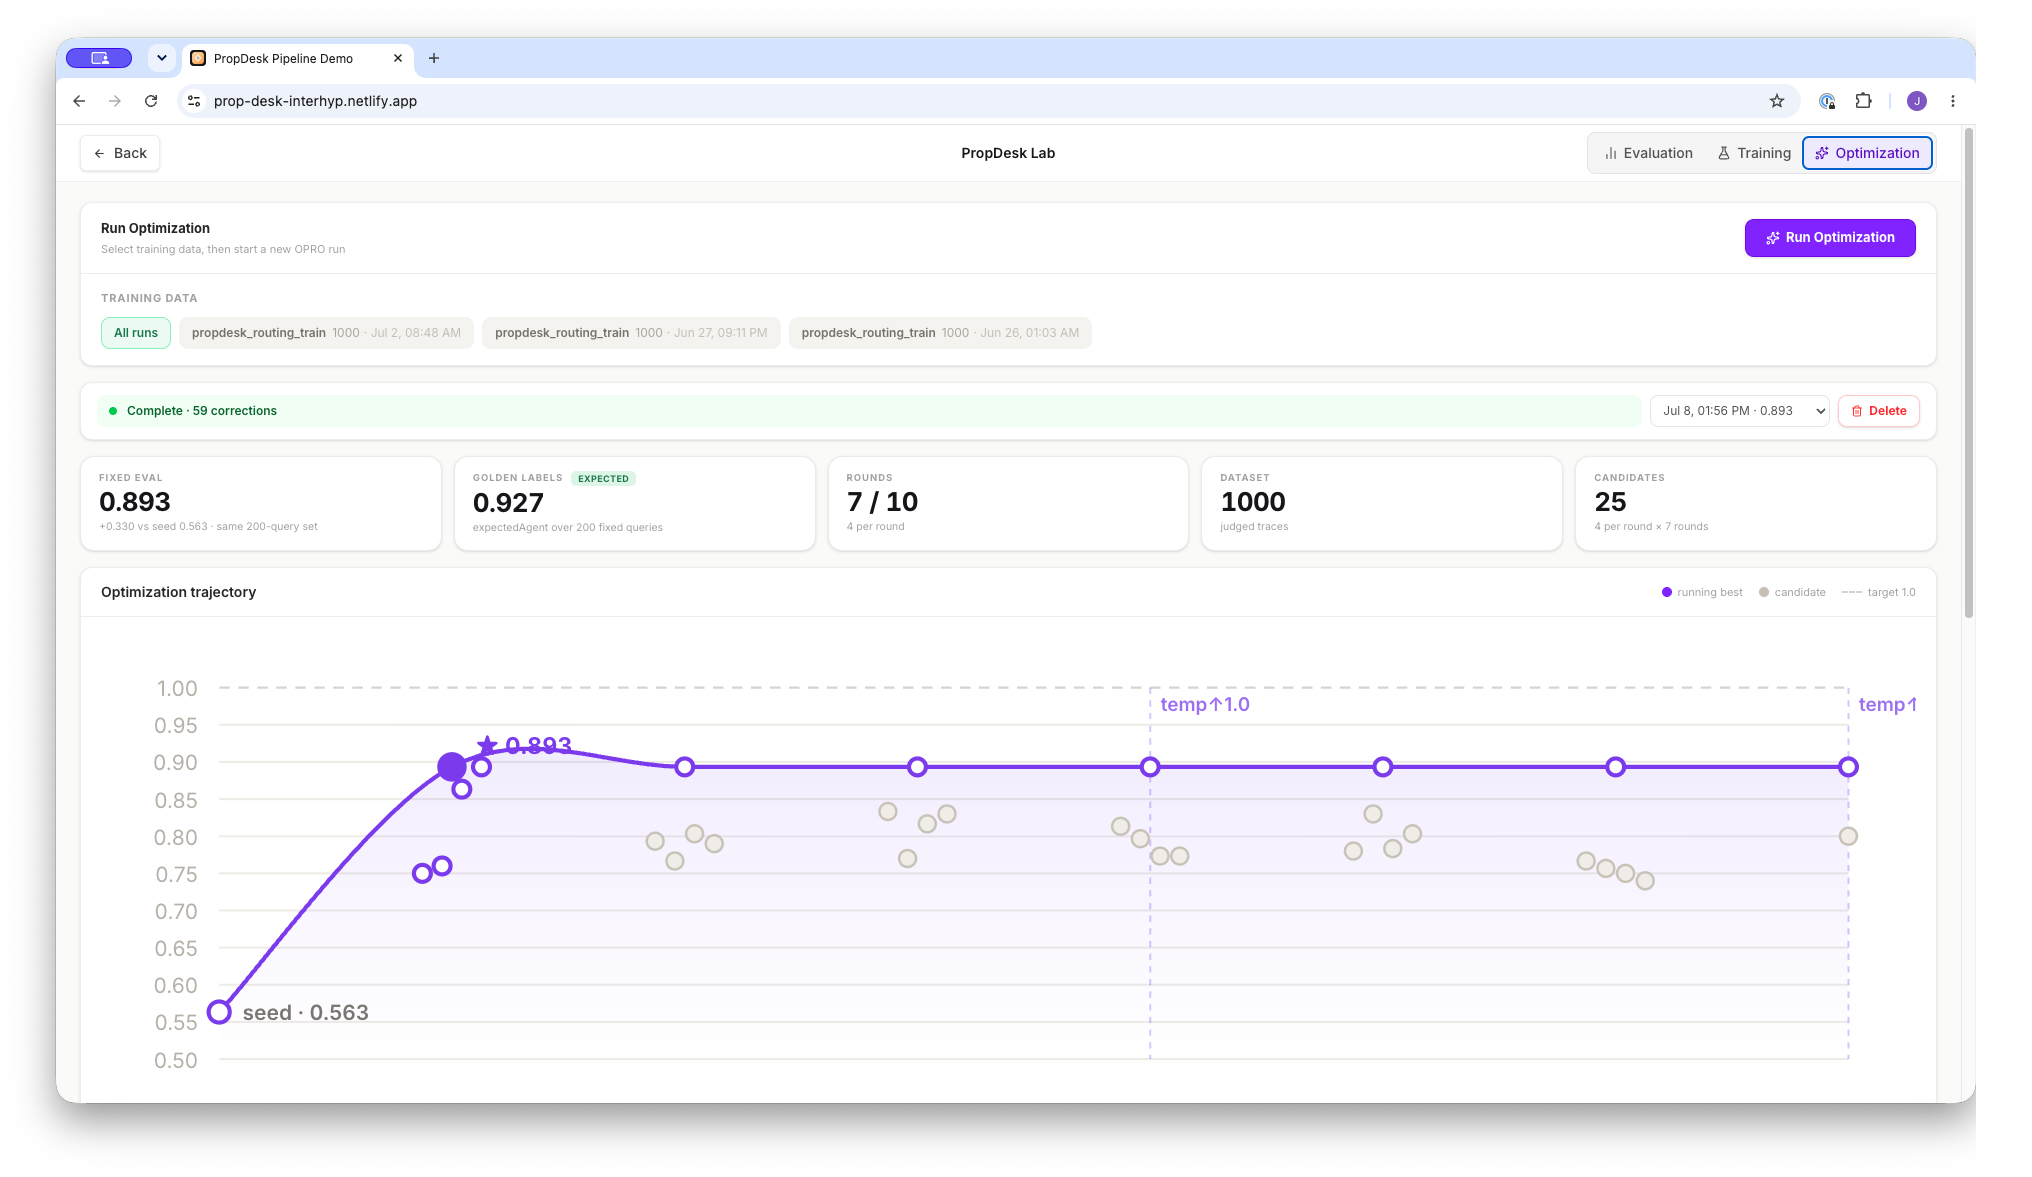
\includegraphics[keepaspectratio]{assets/application/optimization-run.png}}
\caption{Optimization trajectory showing the seed, candidate scores, and best fixed-evaluation result}
\label{fig:application-optimization}
\end{figure}

Together, the views create a traceable improvement cycle: training provides corrections and optimization inputs, optimization produces versioned candidates, and evaluation compares them on a fixed basis. Configuration snapshots, prompt lineage, and immutable run datasets allow users to move from aggregate results back to the runs and traces on which they depend.

The interface consequently distinguishes three actions that could otherwise be conflated. Evaluation measures a selected configuration without modifying the Stage 1 index. Training processes labelled examples and can contribute corrections to that index. Optimization searches for a stronger Stage 2 prompt but does not automatically replace the deployed version. Making these transitions explicit supports controlled experimentation and prevents a completed run from being mistaken for an automatically accepted system change.


\clearpage
\suppressfloats[t]
\section{Sprint-by-Sprint Analysis}\label{sec:sprint-analysis}

\authoredsubsection{Sprint 1}{Julius}{Julius Bethge}\label{sec:sprint1}

\subsubsection{Sprint Goal and Planning}\label{sec:sprint1-goal}

Sprint 1 ran from 28 April to 11 May 2026, with Julius acting as Scrum Master. Following the preliminary organization in Sprint 0, it focused on setting up the working environment, conducting the initial research, forming a first view of the pipeline architecture, and taking the first steps toward the showcase interface. The sprint goal combined five workstreams: establishing the project and development environment, delivering a first showcase-application increment, clarifying access to suitable language models, defining relevant evaluation metrics, and deriving an initial pipeline architecture from scientific research. The sprint was initially planned with 25 story points, corresponding to five points for each team member. Its purpose was to reduce the principal uncertainties of the project rather than to deliver a complete pipeline.

Responsibilities followed the main components: Marco established Jira and researched judges and their biases; Julius created the repositories and initial application and coordinated the sprint; Mohsin investigated model providers; Sebastian covered local models and routing; and Gáspár developed the metrics and optimizer research. The architecture, MVP, repository strategy, and Sprint Review were collaborative.

\Cref{fig:sprint1-backlog} shows the six work items recorded in Jira at the end of the sprint, including the additional two-point task for establishing a local LLM setup after no external token provider was available.

\begin{figure}
\centering
\pandocbounded{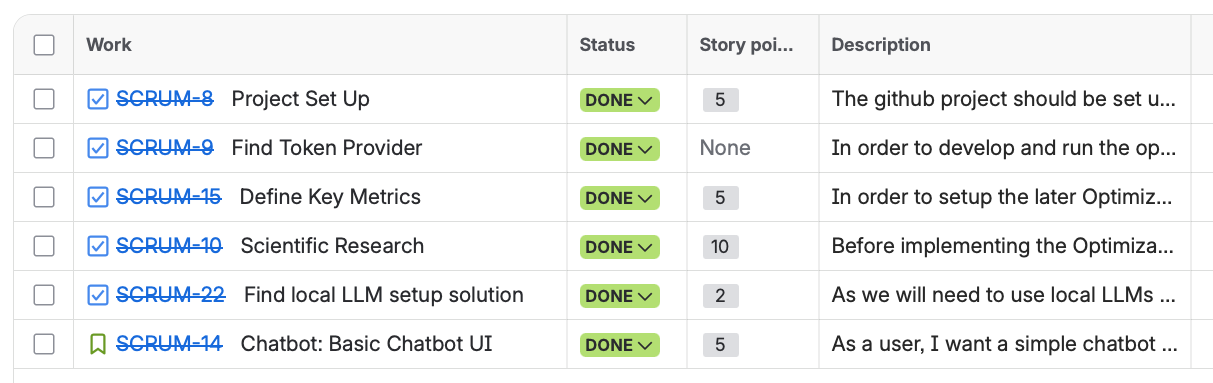
\includegraphics[keepaspectratio]{assets/sprints/sprint1-backlog.png}}
\caption{Sprint 1 backlog in Jira showing story-point estimates and completion status.}
\label{fig:sprint1-backlog}
\end{figure}

\subsubsection{Implementation and Sprint Execution}\label{sec:sprint1-execution}

The team created the \texttt{LMUxInterhyp} GitHub organization with two repositories serving different purposes. The \texttt{pipeline} repository provided an experimental environment for rapidly exploring Router, judge, and optimization approaches. The \texttt{chatbot} repository formed the maintainable codebase for the integrated showcase application. Validated ideas could therefore be reimplemented in the application without treating exploratory Python code as its foundation. Jira issues were linked to branches and pull requests, supported by automated checks and preview deployments.

The first application increment combined a React and TypeScript frontend with a Convex backend. It already allowed a user to submit a query and receive an LLM-generated answer. Ollama supported local execution, while OpenRouter was available for the first deployed setup. The increment established the technical basis for the showcase application, but it did not yet contain the multi-stage Router, judge, or optimizer.

Model access was a critical dependency because the Router, agents, judge, and optimizer could each require inference. Neither Interhyp nor the university could provide the required tokens. The team therefore selected Ollama as the initial local runtime and documented suitable models and setup instructions. This removed the immediate dependency on an external API budget. It was not intended as a permanent architectural restriction because the planned components could require different model capabilities.

The metric work translated the objective into routing quality, latency, and cost. Candidate measures included routing accuracy, agent-level precision and recall, clarification behavior, Router latency, and token cost. Broader measures included first-touch resolution and cost per successful outcome. Because Interhyp reported uneven agent usage, aggregate accuracy could conceal weak performance on less frequent agents. Weighted and agent-level results were therefore retained for later evaluation, while no combined optimization metric was fixed during this sprint.

Research covered multi-agent routing, LLM-based evaluation, judge bias, prompt optimization, and self-improving pipelines. The team used these workstreams to compare possible approaches and translate them into requirements for the initial architecture. The resulting proposal treated routing as a decision involving quality, latency, and cost, considered an independent judge as a source of evaluation signals, and investigated automated prompt optimization as an alternative to repeated manual refinement. Judge panels and more advanced learning approaches were retained as possible extensions rather than included in the initial MVP.

The initial production-path concept used a Router to select the specialist agent best suited to a user query. The selected agent would generate the response returned to the user, while alternative agents remained available for other request types.

\begin{figure}
\centering
\pandocbounded{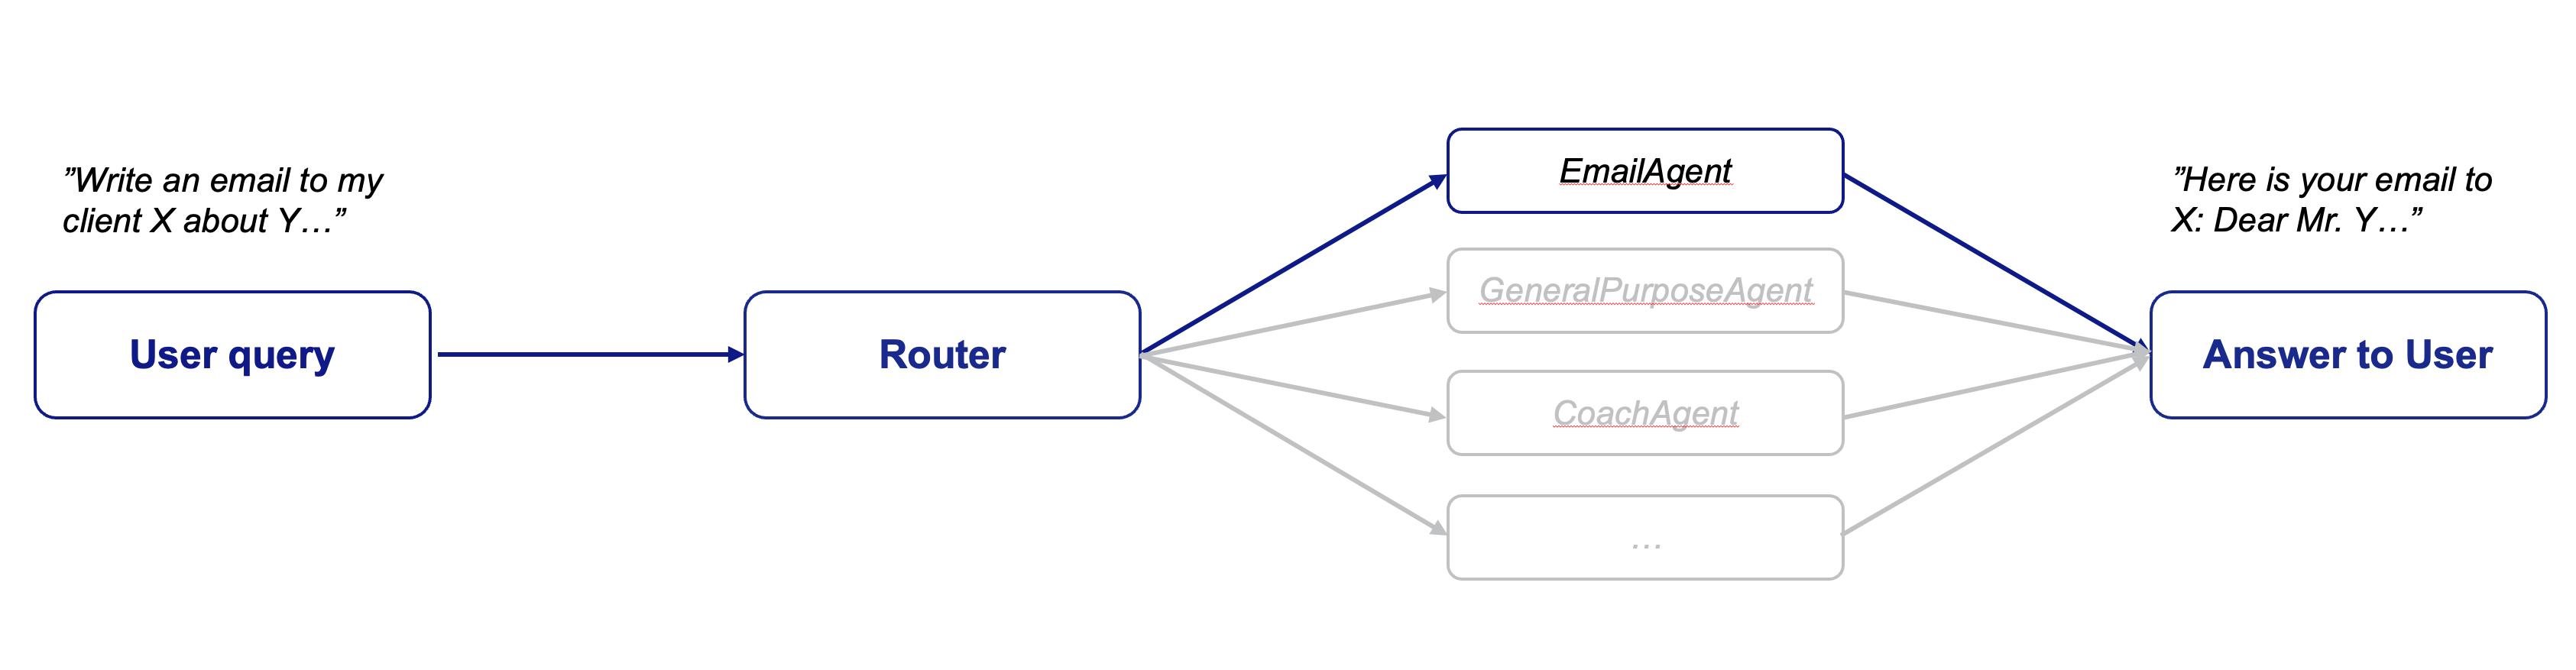
\includegraphics[keepaspectratio]{assets/sprints/sprint1-production-path.png}}
\caption{Initial Sprint 1 production path from a user query to the selected specialist agent's response.}
\label{fig:sprint1-production-path}
\end{figure}

The broader proposal extended this production path with a separate asynchronous pipeline. The live path would route a query and return an agent answer without waiting for evaluation. It would also create a structured trace containing the query, routing decision, candidate information, and answer. The asynchronous path could compare alternative outcomes, derive evaluation signals through an independent judge, and optimize the Router prompt. Resulting changes would require validation before deployment.

\subsubsection{Sprint Review}\label{sec:sprint1-review}

The Sprint Review took place on 12 May 2026 with our Interhyp partners. During the sprint, the lack of provided inference tokens had made an additional local-model setup task necessary. This increased the scope from 25 to 27 story points. All 27 points were completed. The team presented the project and repository setup, first chatbot increment, metric proposal, scientific findings, initial architecture, and MVP boundary.

\Cref{fig:sprint1-burndown} shows the scope increase and the completion of all committed work by the end of the sprint.

\begin{figure}
\centering
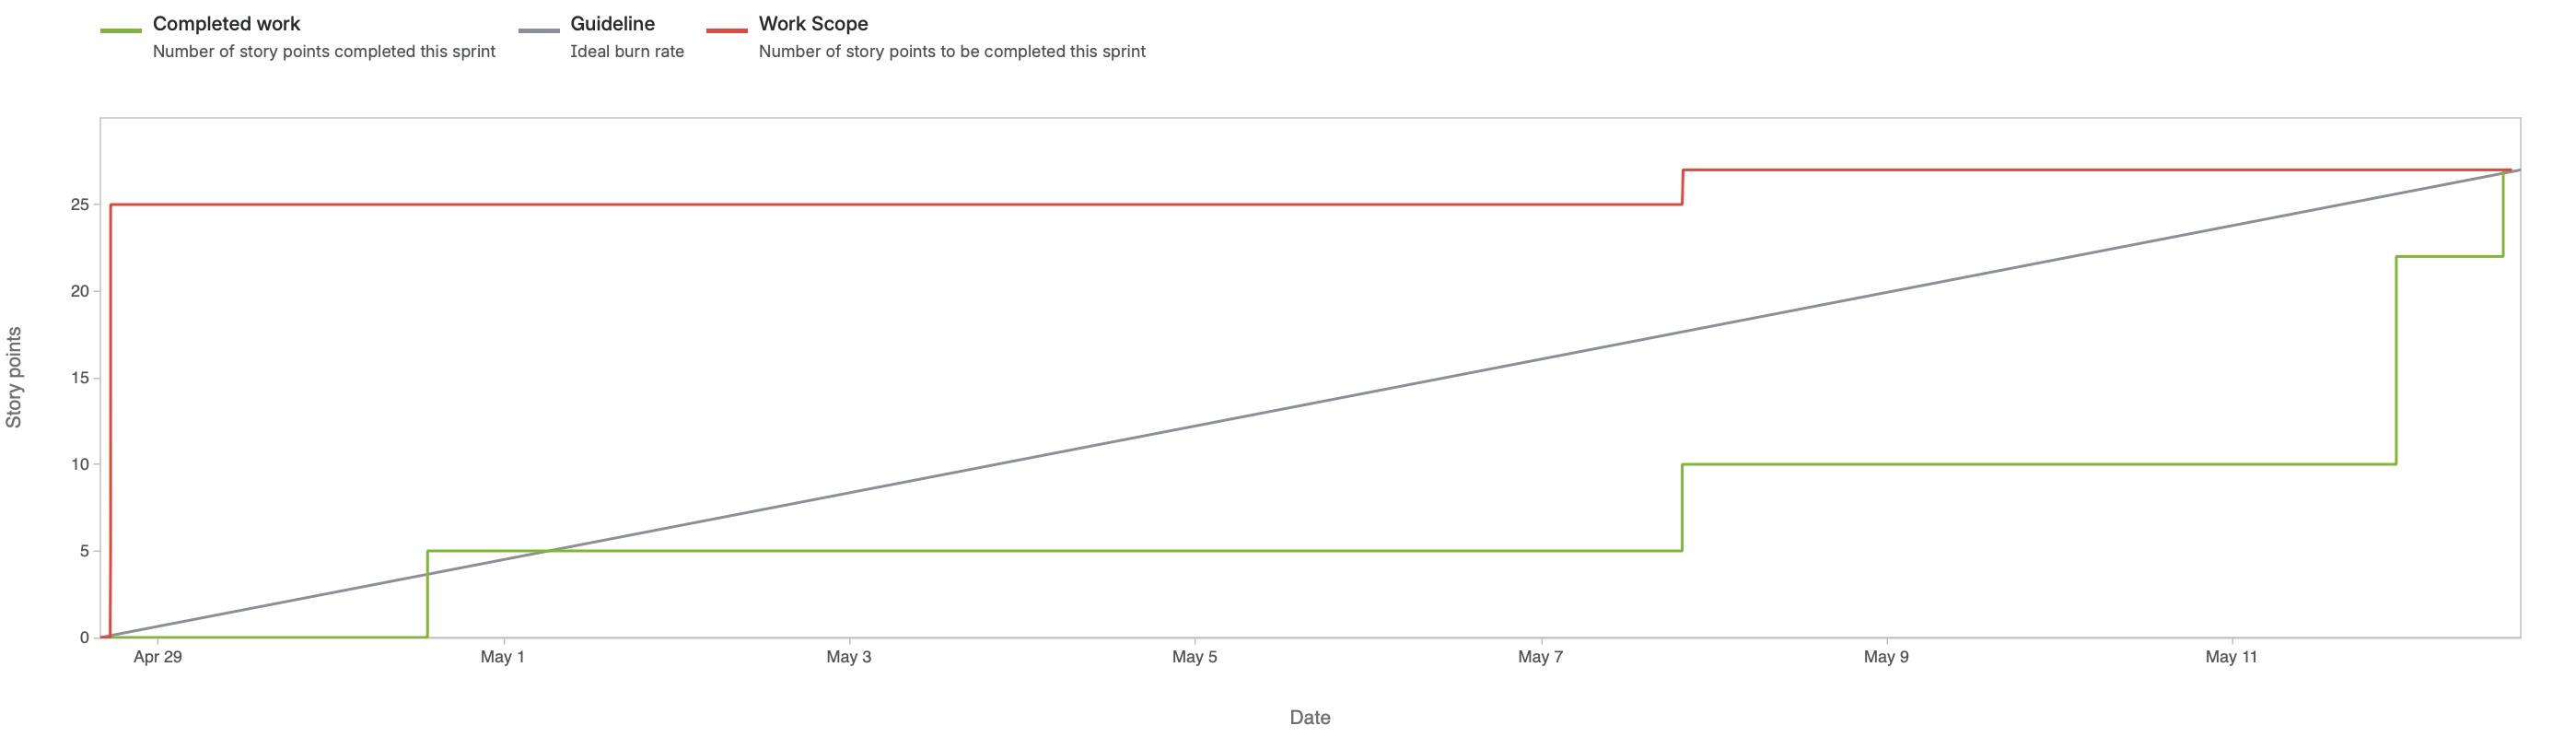
\includegraphics[width=1\linewidth,height=\textheight,keepaspectratio]{assets/sprints/sprint1-burndown.png}
\caption{Sprint 1 burnup chart.}\label{fig:sprint1-burndown}
\end{figure}

The discussion concentrated on the architecture rather than on the basic chatbot interface. Interhyp considered the separation between the live application path and asynchronous evaluation and optimization a suitable basis for the following sprints. They also supported the MVP approach, which prioritized a smaller executable pipeline before more advanced routing and judge concepts. At the same time, the architecture remained open to revision as the components were implemented and evaluated.

The review also reinforced the need to interpret accuracy in the context of unequal agent usage. This supported the planned use of agent-level and potentially weighted evaluation alongside aggregate results. Overall, the positive review allowed Sprint 2 to move from setup and architectural reasoning toward the first implementation of the pipeline components, data, Router, judge, and optimizer.

\subsubsection{Sprint Retrospective}\label{sec:sprint1-retrospective}

The retrospective showed high motivation, broad participation, and productive collaboration. Team members particularly valued the brainstorming process, the effective division of work, and the contributions to the research and architecture. These strengths had enabled the team to address several foundational questions within one sprint and to present a coherent direction despite the unresolved model-access issue at its beginning.

The team nevertheless identified a need for clearer task delegation, better-prepared meeting agendas, and more opportunities for in-person work. It also concluded that meetings with Interhyp should make more active use of the partners' expertise. Rather than primarily presenting progress, the team wanted to prepare concrete questions and alternatives that could be discussed with them. The complete feedback board is shown in \cref{fig:sprint1-retrospective-feedback}.

\begin{center}
\centering
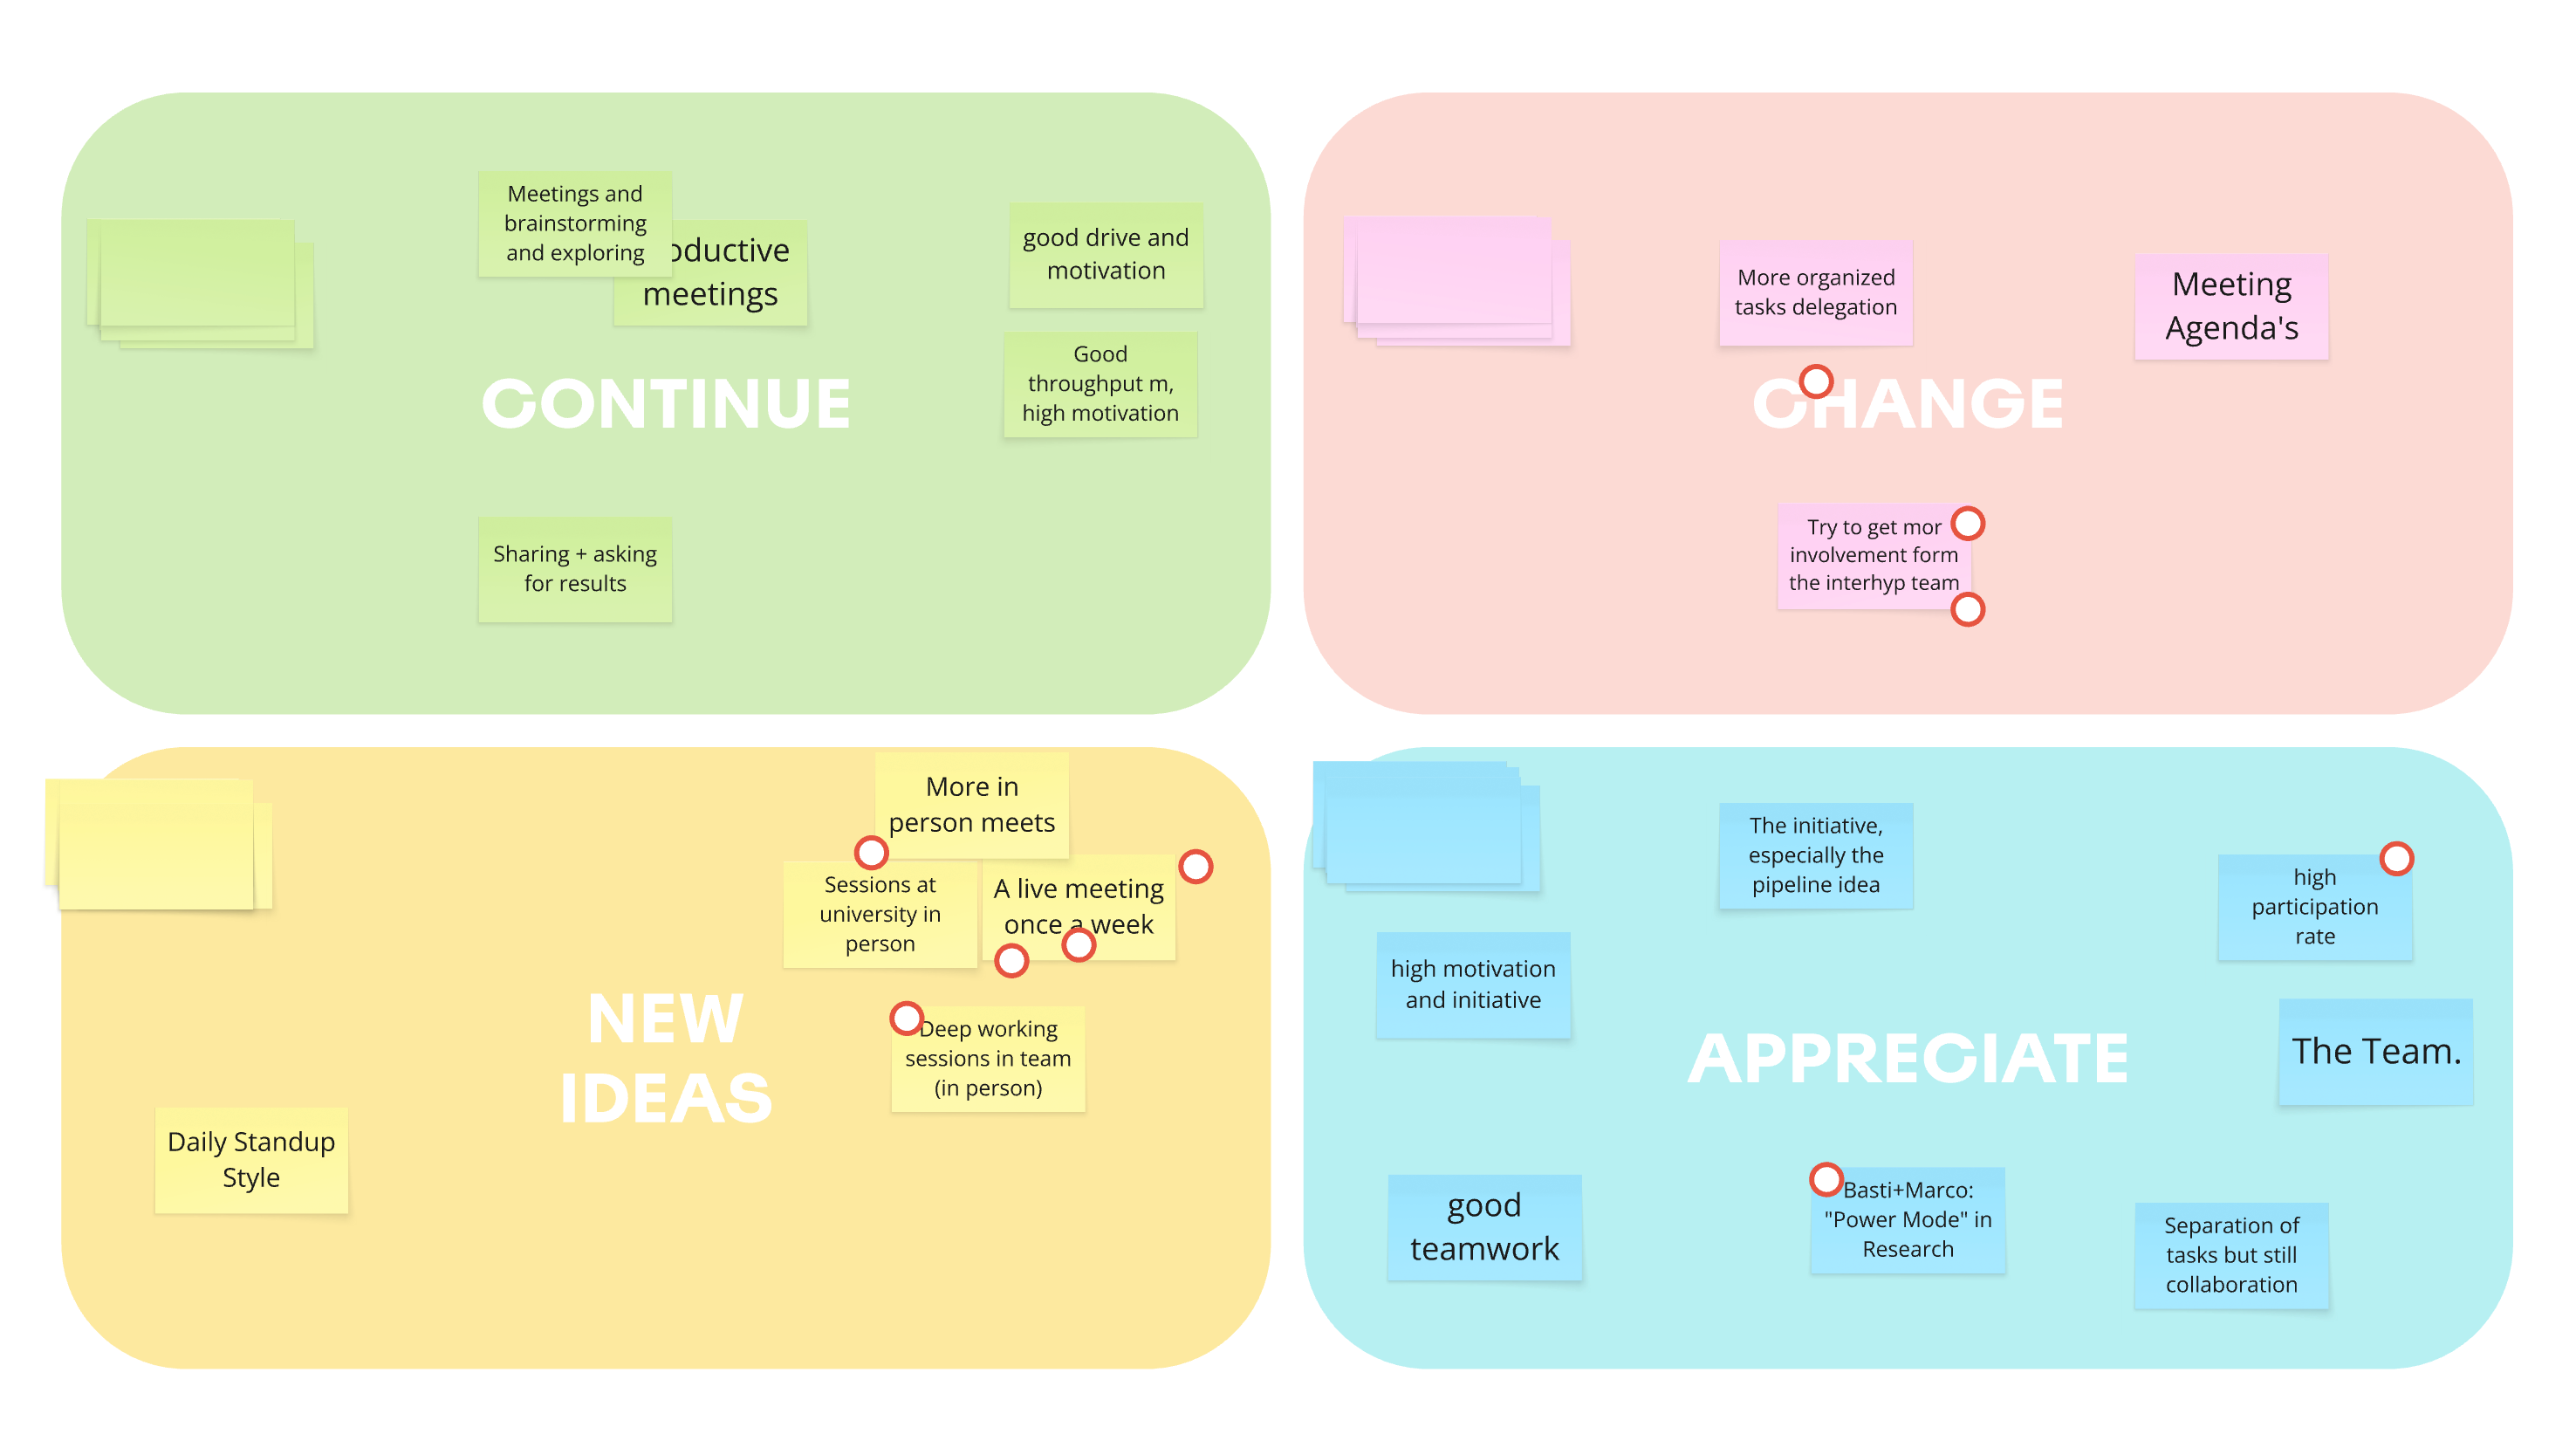
\includegraphics[width=1\linewidth,height=\textheight,keepaspectratio]{assets/sprints/sprint1-retrospective-feedback.png}
\captionof{figure}{Sprint 1 retrospective board showing feedback grouped as Continue, Change, New Ideas, and Appreciate.}
\label{fig:sprint1-retrospective-feedback}
\end{center}

Two actions were adopted for Sprint 2. First, a recurring in-person working session on Tuesdays would provide time for deeper collaboration and architectural alignment. Second, Interhyp meetings would be prepared as focused discussion and feedback sessions. These changes were intended to improve shared understanding within the team, shorten coordination paths, and incorporate domain feedback earlier into technical decisions. \Cref{fig:sprint1-retrospective-actions} records the owners and deadlines agreed for both actions.

\begin{center}
\centering
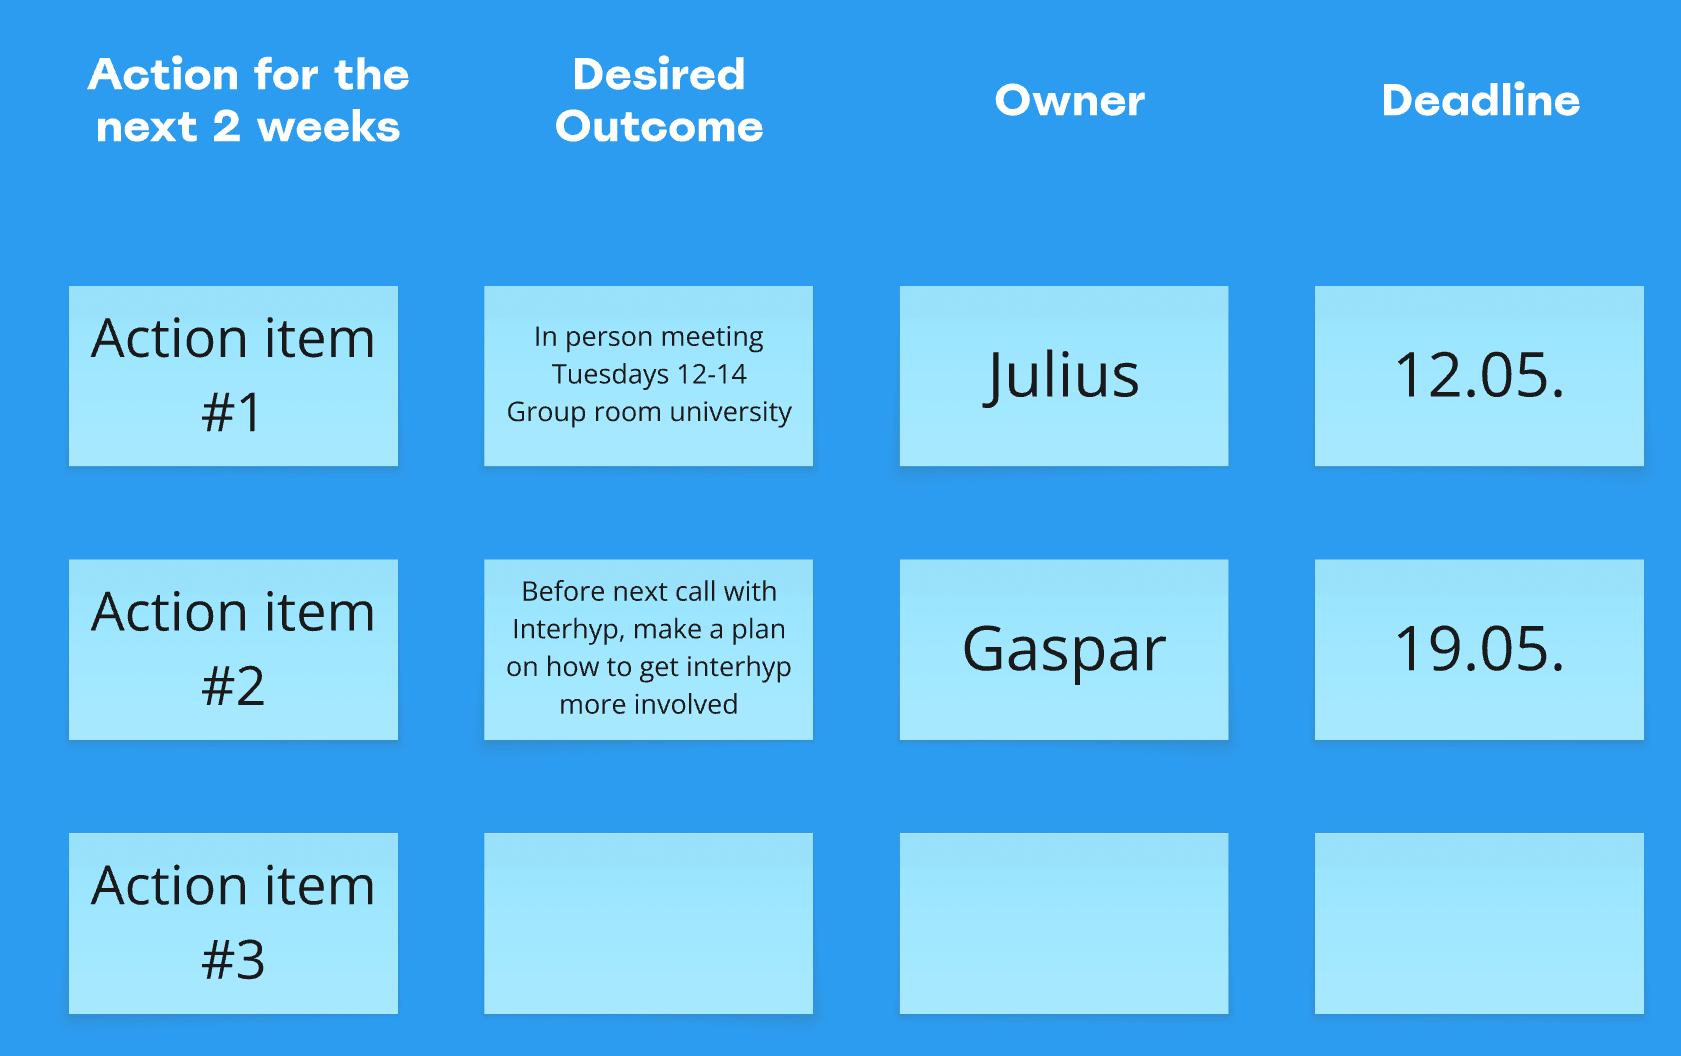
\includegraphics[width=1\linewidth,height=\textheight,keepaspectratio]{assets/sprints/sprint1-retrospective-actions.png}
\captionof{figure}{Sprint 1 retrospective action items showing owners and deadlines.}
\label{fig:sprint1-retrospective-actions}
\end{center}


\subsection{Sprint 2}\label{sec:sprint2}
\pendingcontent{Gáspár Harmati}{Insert the Sprint 2 goals, planning, implementation and execution, review, retrospective, and supporting Jira or retrospective figures.}

\begin{figure}
\centering
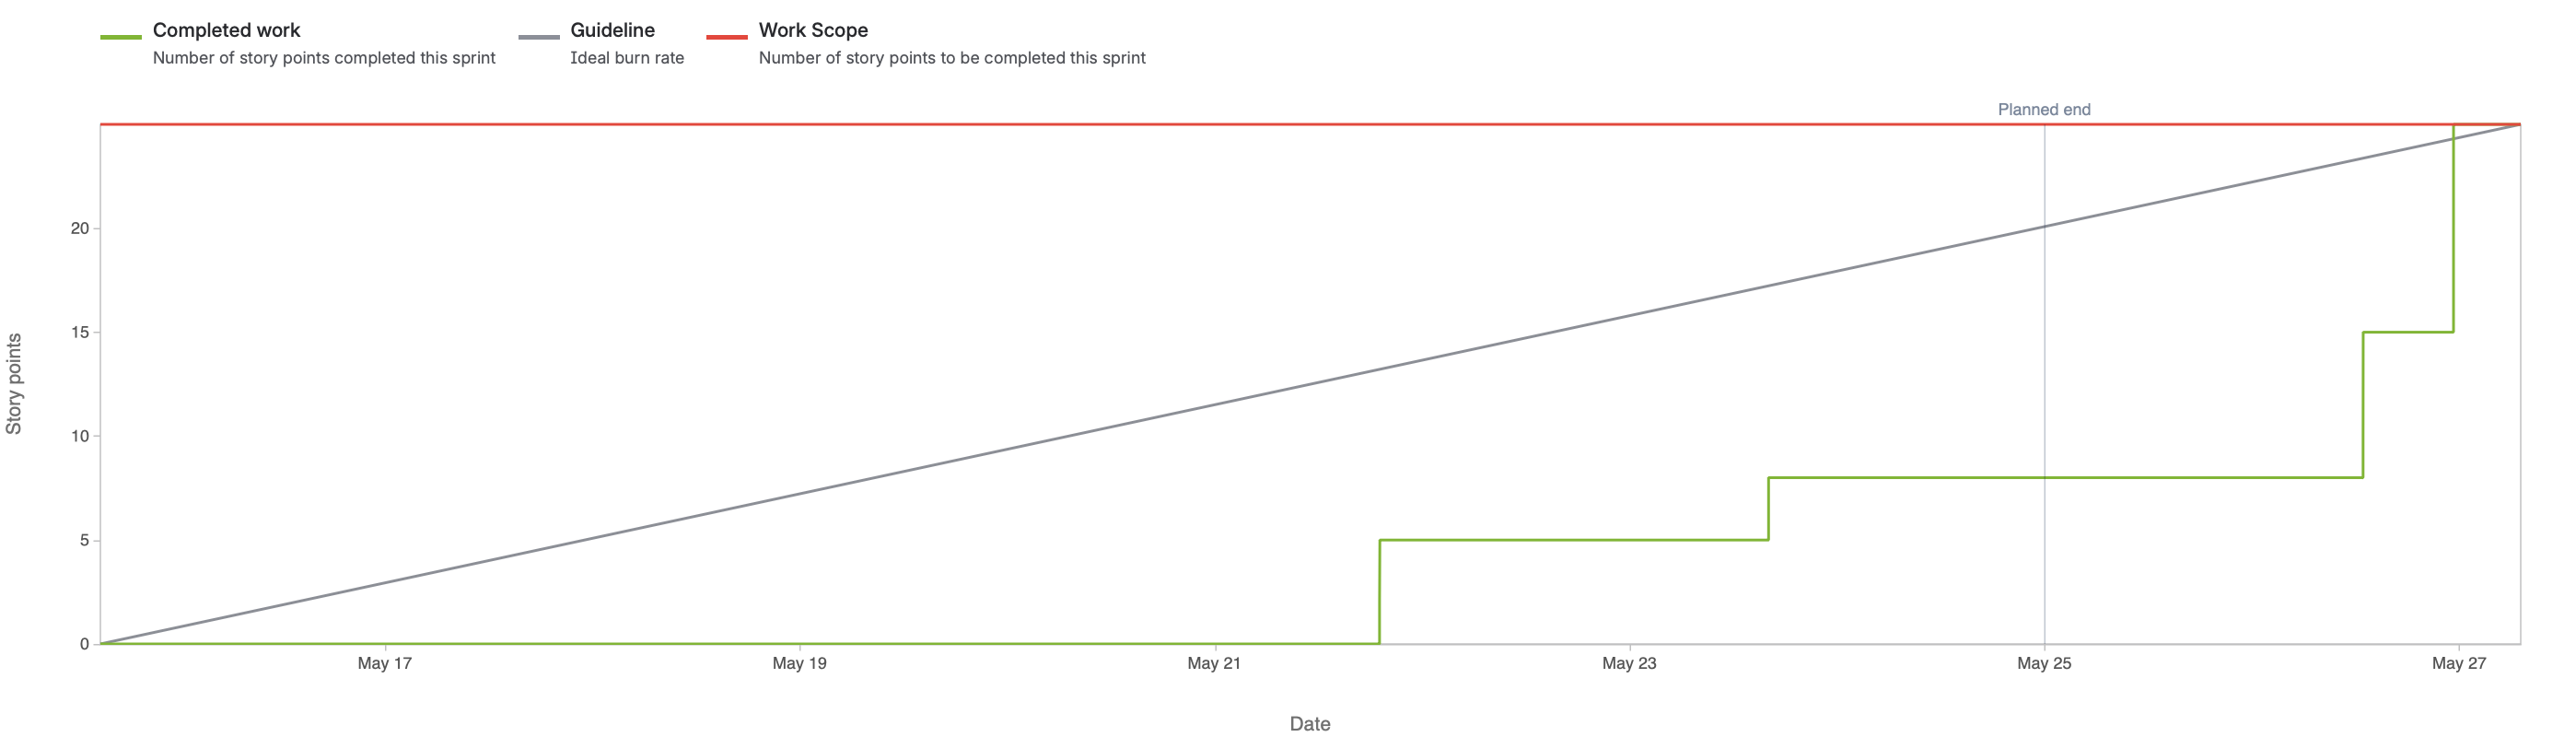
\includegraphics[width=1\linewidth,height=\textheight,keepaspectratio]{assets/sprints/sprint2-burndown.png}
\caption{Sprint 2 burndown chart.}\label{fig:sprint2-burndown}
\end{figure}

\authoredsubsection{Sprint 3}{Marco}{Marco-Fabian Schröder}\label{sec:sprint3}

Sprint 3 ran from 26 May to 09 June 2026, with the review and retrospective held on 09 June. Sprint 2 had established the main pipeline components as separate, independently functional modules, so the objective of this sprint was to shift from further improving individual capability in the first half toward preparing these modules for integration into a single executable loop in the second half of the sprint. Two open questions shaped the work: how to optimize the router's two stages separately, and how to redesign the judge to reduce the systematic biases identified in its first evaluation. In addition, Interhyp had encouraged the team during the Sprint 2 review to prioritize measurable evaluation results over further scope expansion, which set the tone for the sprint. Marco Schröder took over the role of the Scrum Master for this sprint.

\subsubsection{Sprint Goals}\label{sec:sprint3-goals}

The team committed to creating a new evaluation dataset with more challenging routing cases and to validating and improving the judge until its evaluations are more accurate than the router's decisions. For the router, the goal was to find suitable per-agent thresholds for Stage 1 and to build a dashboard that visualizes the effect of different threshold settings on accuracy and latency. The sprint further included a proof of concept of the optimizer with the DSPy optimization framework and the preparation of the end-to-end integration of router, judge, and optimizer on a data format level toward a first optimization run producing an improved router prompt. The team also prepared the mid-term presentation within this sprint.

\subsubsection{Sprint Planning}\label{sec:sprint3-planning}

The team decided that the increasing maturity of the individual components justified restructuring the backlog into component-oriented epics for the router, judge, optimizer, and documentation work. Backlog items were deliberately kept small, with a maximum estimate of three story points per item, to promote fast intermediate deliveries and early discussions on the integration. The sprint contained 25 story points in total, consistent with the velocity of the previous sprints. The established stand-up cadence was retained, with the Sunday stand-up moved to the morning and extended to one hour to give the team more preparation time ahead of the mid-term presentation.

\Cref{fig:sprint3-backlog} shows the user stories that were included in the sprint backlog for Sprint 3. The only item which had a story point estimate of more than three story points was the preparation of the slides for the mid-term presentation with five story points, but this was equally split across the team through subtasks with one story point per team member.

\begin{figure}
\centering
\pandocbounded{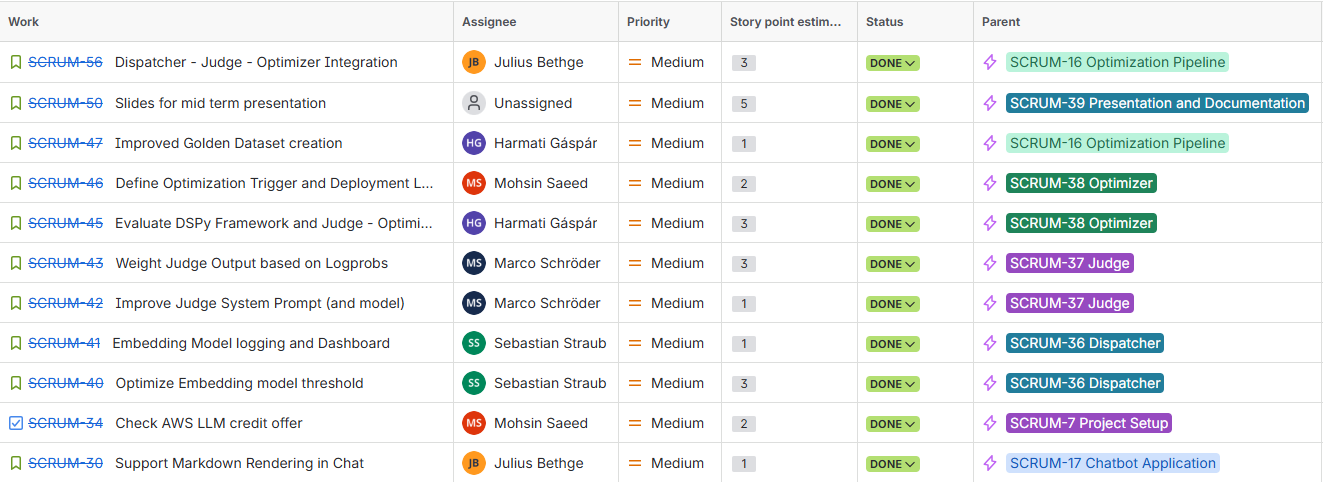
\includegraphics[keepaspectratio]{assets/sprints/sprint3-backlog.png}}
\caption{Sprint 3 Backlog in Jira with owners and completion status.}
\label{fig:sprint3-backlog}
\end{figure}


\subsubsection{Implementation and Execution}\label{sec:sprint3-execution}

The largest block of work concerned the router's first stage. Its reference store was redesigned from formal agent descriptions to sets of example queries per agent, since embedding models perform more reliably on semantically symmetric inputs such as query-to-query comparisons than on asymmetric pairs of short queries that are compared to long descriptions \autocite{gao2023hyde}. The embedding model itself was upgraded from BAAI/bge-small-en-v1.5 to intfloat/multilingual-e5-large, guided by the Massive Text Embedding Benchmark \autocite{muennighoff2023mteb}, while keeping Stage 1 latency at approximately 100 ms. Even higher performing models were not selected due to external API dependencies that would have introduced per-query cost. The thresholding logic was revised from a single global threshold to per-agent margin thresholds between the top two candidates, calibrated on 1,000 queries from the golden dataset. In addition, the full similarity vector of all eight agents was logged for every Stage 1 decision. A dashboard visualizes the effect of different threshold settings on routing accuracy and time saved (\cref{fig:sprint3-thresholds}). Following a data-leak warning from the Product Owner Julian, the team decided that new Stage 1 example queries should never originate from the golden dataset as this would lead to artificially perfect results, and a separate dataset of 250 ambiguous queries was created for this purpose.

\begin{figure}
\centering
\pandocbounded{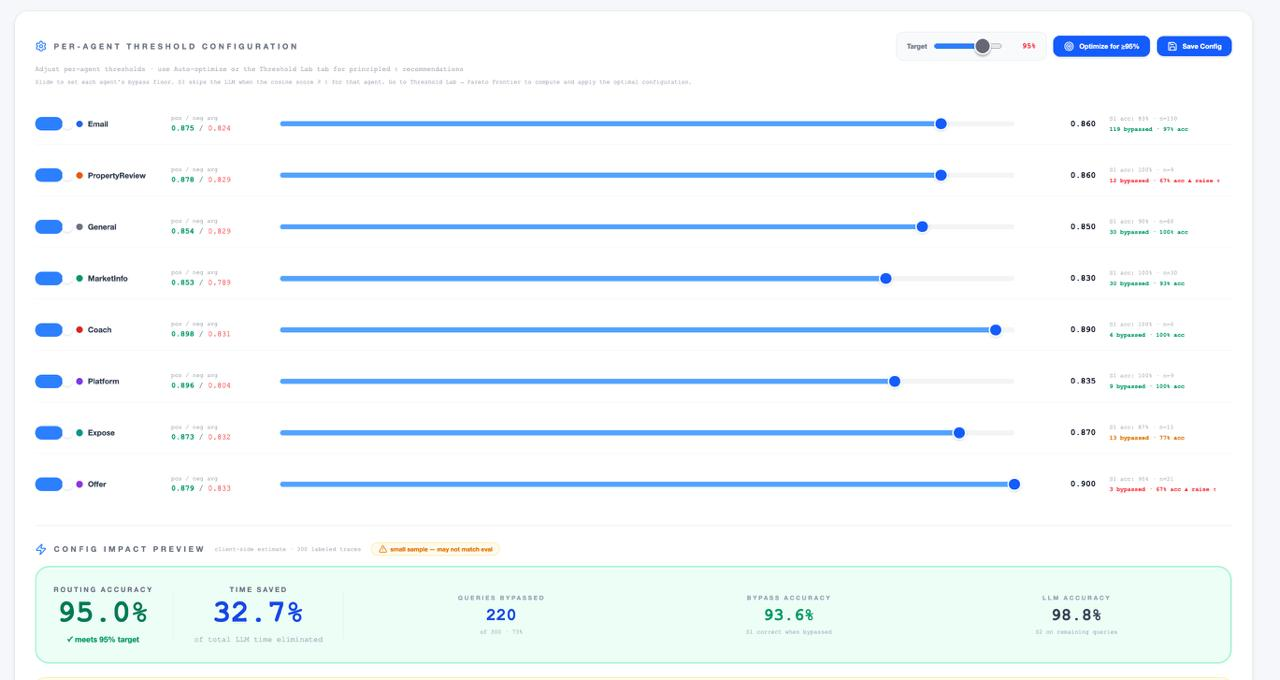
\includegraphics[keepaspectratio]{assets/sprints/sprint3-threshold-dashboard.png}}
\caption{Dashboard for exploring per-agent margin thresholds in Stage 1.}
\label{fig:sprint3-thresholds}
\end{figure}


The second focus was the redesign of the judge. Its first evaluation, run with a generic comparison prompt on Gemma 4 31B, reached only 51\% agreement with the ground truth on the 100 most uncertain queries, and the root cause analysis identified a systematic style bias toward the highly formatted responses of the MarketInfoAgent. The prompt was redesigned around routing-specific evaluation rubrics that are applied in a sequential, form-filling scheme. After the AWS Bedrock access was validated and ensured in this sprint, the judge model was additionally migrated to Claude Sonnet 4.6 under a hybrid architecture in which the router continues to run locally while compute-intensive components use cloud models. This raised judge accuracy to 98\% on the training dataset and 99\% on the evaluation dataset. An exploration of token log-probabilities as a judge confidence signal was closed without result. The evaluated model commits to its decision internally before generating the output, so the log-probabilities degenerate to complete certainty values of 100\% for the winning agent that carry no usable information.

In parallel, the team evaluated the DSPy framework \autocite{khattab2024dspy} as a possible replacement for the self-built OPRO optimizer. The proof of concept used its MIPROv2 optimizer and a deployment guard that rolls back any new prompt below a two-percentage-point improvement. The optimized prompt scored identically to the baseline, which exposed a conceptual issue rather than a tuning problem: the evaluation ran through both Stages of the router, so Stage 1 resolved nearly all validation queries before the optimized Stage 2 prompt was ever exercised. This led to the result that not enough queries were evaluated to produce statistically relevant insights. The knowledge that optimization runs must target Stage 2 directly was carried into the next sprint, together with the pending decision between DSPy and the self-built optimizer. The story for the DSPy optimizer was still closed as a PoC integrating the framework was set up.

Finally, the sprint laid the groundwork for integration. The team mapped all module interfaces in an in-person whiteboard session and connected the pipeline through three links: the judge runs as an asynchronous background process on every router request, its corrections are written to an isolated correction file that mirrors the Stage 1 example format without contaminating it, and the optimizer is triggered manually using the judge's output data format so that generated prompts can be reviewed before deployment. The proposal by Julius to replace this direct coupling with a dedicated orchestration layer to ensure the integration of the pipeline into the Chatbot application became the main priority for Sprint 4.

\subsubsection{Sprint Review}\label{sec:sprint3-review}

The review took place at the Interhyp office on 09 June 2026 and was extended to two hours, with additional colleagues of Julian and Rainer joining the second half of the meeting so that the team could practice the mid-term presentation and gather broader technical feedback. Julian and Rainer appreciated the threshold dashboard for making the tradeoff between routing accuracy and time saved immediately visible and were interested in exploring an optimization approach for the per-agent thresholds themselves in the future. They emphasized that the pipeline stands or falls with the judge and cautioned that, as router accuracy improves, a stagnating judge could begin to drag accuracy down rather than lift it. The team agreed that in a production setting it would be required to periodically re-evaluate the judge on newly labeled queries. The audience additionally proposed crowdsourcing ambiguous router cases by letting chatbot users choose between the two best agent responses, which would distribute annotation effort across all users and offer a possibility in the production system to evaluate the judge's performance.

All 25 story points were completed. The burndown chart (\cref{fig:sprint3-burndown}) shows three conspicuous patterns. It starts from a zero baseline because the sprint was technically started immediately after the old sprint was closed in Jira, but the sprint planning session still had to be conducted. As during the sprint planning session all items were moved to the sprint backlog, there is an increase of 25 story points one day after the sprint started. Second, there is a slight increase and immediate decrease in story points one day after the sprint planning happened as the DSPy optimizer PoC turned out to be more complex than expected, but at the same time the creation of additional ground truth queries required less effort than estimated as the same procedure had already been performed in the previous sprint. Also, most items were closed in the second half, which reflects the dependency of the integration work on the completion of the individual module tickets.

\begin{figure}
\centering
\pandocbounded{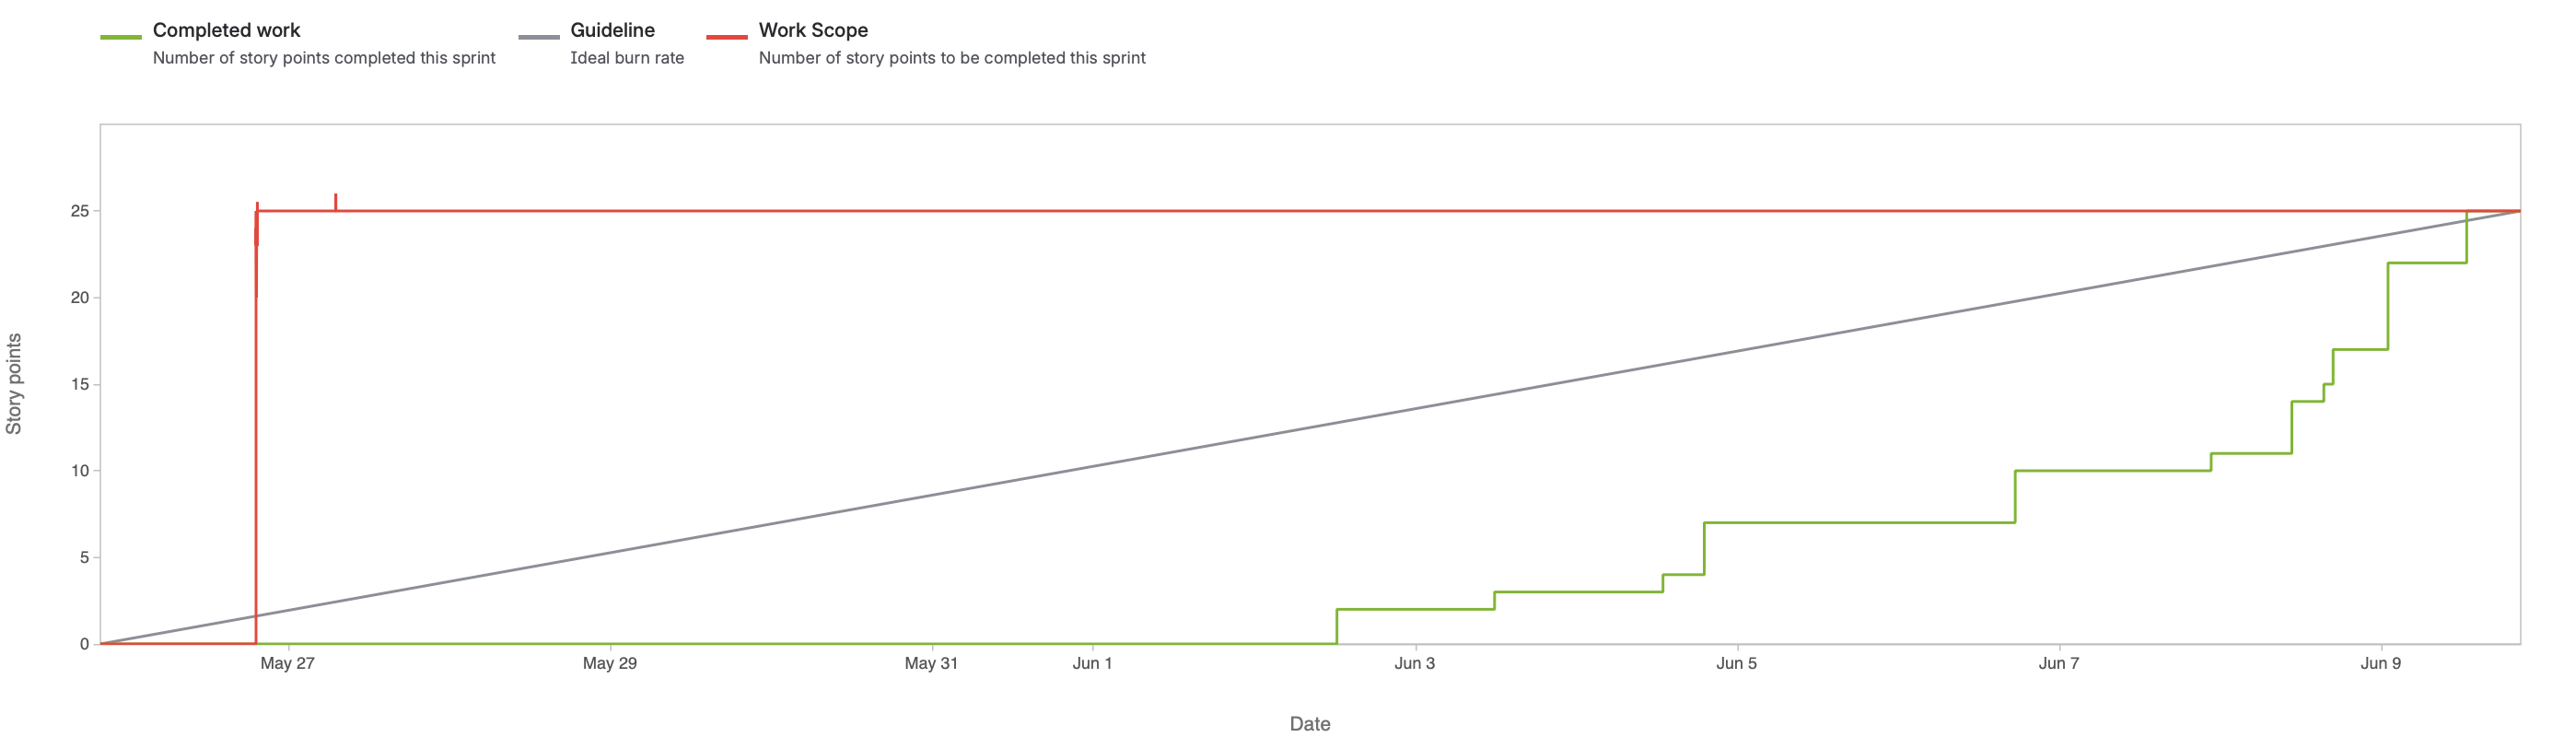
\includegraphics[keepaspectratio]{assets/sprints/sprint3-burndown.png}}
\caption{Sprint 3 burndown chart.}
\label{fig:sprint3-burndown}
\end{figure}


\subsubsection{Sprint Retrospective}\label{sec:sprint3-retrospective}

The sprint retrospective was held on 09 June 2026, directly after the sprint review meeting. In the opening exercise, team members reviewed the sprint in the style of a product review on Amazon with a star rating, which converged on three to four out of five stars. The sprint felt productive but stressful and at times messy, mainly because preparing the integration revealed more architectural complexity than the estimates had anticipated. A lot of discussions were happening based on ad-hoc and late-night calls to clarify misunderstandings about the individual module outputs. The team concluded that user stories need to be discussed in more detail during planning to reach realistic estimates (\cref{fig:sprint3-retrospective}).

\begin{figure}
\centering
\pandocbounded{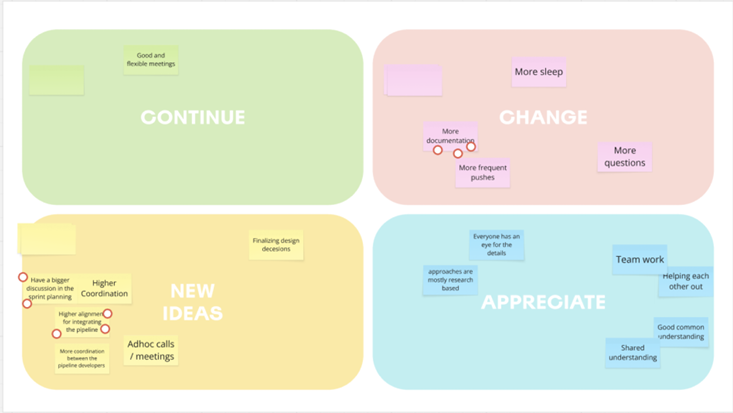
\includegraphics[keepaspectratio]{assets/sprints/sprint3-retrospective.png}}
\caption{Sprint 3 retrospective feedback collection in Miro.}
\label{fig:sprint3-retrospective}
\end{figure}


Two action items were derived for the following sprint: a dedicated meeting on the functional integration of the modules directly after the mid-term presentation, and an increase to four meetings per week, including a Monday evening slot to clarify open questions ahead of the weekly in-person session (\cref{fig:sprint3-actions}).

\begin{figure}
\centering
\pandocbounded{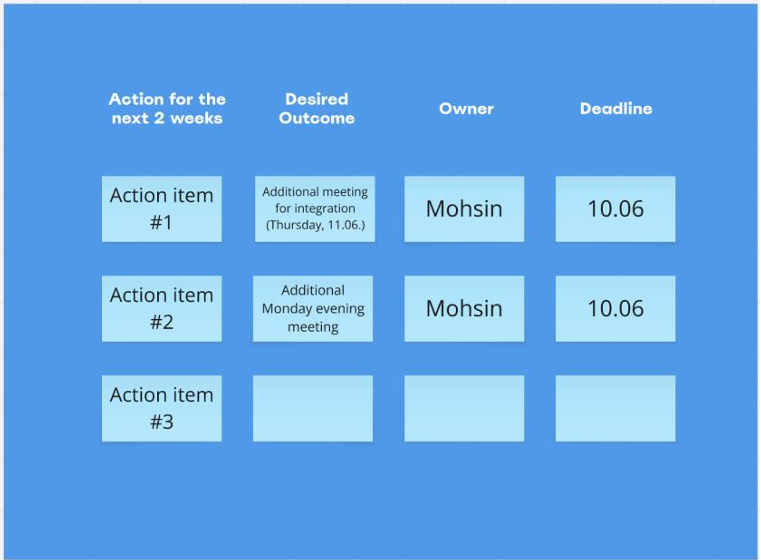
\includegraphics[keepaspectratio]{assets/sprints/sprint3-action-items.png}}
\caption{Action items for Sprint 4.}
\label{fig:sprint3-actions}
\end{figure}

\authoredsubsection{Sprint 4}{Mohsin}{Mohsin Saeed}\label{sec:sprint4}

Sprint 4 ran from 10 to 23 June 2026, with the review on 24 June, and marked the transition from independently functioning components to a unified system. By the end of Sprint 3 the router, judge, and optimizer each worked on their own but still communicated through direct subprocess calls and local JSON files, so any change to one module risked breaking the others. Sprint 4 set out to replace that fragile arrangement with an integrated, end-to-end pipeline that could be run, observed, and evaluated as one system. Mohsin Saeed served as the Scrum Master for this sprint.

\subsubsection{Sprint Goals}\label{sec:sprint4-goals}

The sprint goal was to deliver a complete, end-to-end pipeline that a user could run as a unified system, resting on three deliverables: a centralized pipeline skeleton that formally defined the interfaces between all components through a single orchestration layer, a finalized decision between the OPRO and DSPy optimizers together with its integration, and a pipeline visualization dashboard that made every routing and evaluation step inspectable in real time. The goal met the SMART criteria, with a measurable outcome in that a user could submit a query and inspect the full loop, and was time-bound to the two-week sprint ending 23 June 2026 \autocite{schwaber2020scrum}.

\subsubsection{Sprint Planning}\label{sec:sprint4-planning}

The direction had been set at the Sprint 3 review, where Interhyp's product owners, Julian Kappler and Rainer Bomblies, described Sprint 4 as the decisive test of the integrated architecture. The team had already identified the need for an orchestration layer to replace the direct calls between modules. The backlog held seven tickets totaling 25 story points, consistent with prior velocity, but was structured differently (\cref{fig:sprint4-backlog}): the two highest-weight tickets, the pipeline skeleton and the dashboard at eight points each, were treated as shared team efforts spanning the Python worker, the Convex backend, and the React frontend, reflecting how much coordination integration work would demand.

\begin{figure}
\centering
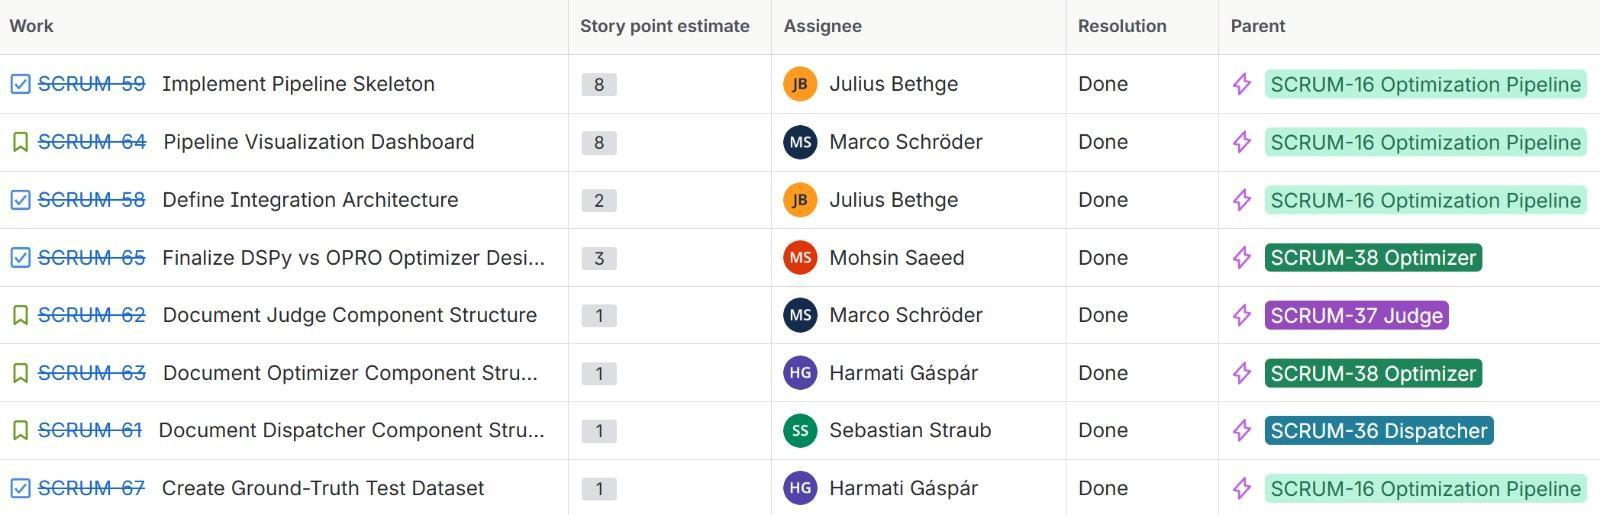
\includegraphics[width=1\linewidth,height=\textheight,keepaspectratio]{assets/sprints/sprint4-backlog.jpg}
\caption{Sprint 4 backlog in Jira, showing the seven tickets and their story-point weights.}\label{fig:sprint4-backlog}
\end{figure}

\subsubsection{Implementation and Execution}\label{sec:sprint4-implementation}

Execution began before any integration code was written, with each module owner documenting their own component on a shared document, so that every member started with a clear picture of the others' modules rather than relying on the ad-hoc explanations that had slowed earlier sprints. During a dedicated design session, the team defined an architecture with three runtime processes: the React frontend renders the UI, Convex manages application state and job scheduling, and the Python worker executes all pipeline logic. Routing all communication through Convex decoupled the components, eliminating the fragility of the Sprint 3 design. Convex was chosen for its real-time streaming, its native vector search on which Stage 1 depends, its typed schema, and its local and hosted deployment support.

On this foundation the team implemented the pipeline skeleton. A Python worker continuously polls Convex, claims the oldest queued job, and executes it across four job types: a chat run, a judge evaluation, a batch run against a labeled dataset, and an optimization run over accumulated judge feedback. Each job maps to a fixed sequence of named steps recorded in Convex, so the frontend always shows what happened, including branches skipped when Stage 1 routed a query directly.

Stage 1 was rebuilt on Convex's vector search: a query is embedded with FastEmbed's multilingual-e5-large model, its nearest neighbors are grouped by agent, and the margin between the top two is compared against a per-agent threshold, with Stage 2 calling Ollama and selecting the agent with the highest log-probability only if the margin is not met. New vector entries are held in memory throughout a batch run and inserted only after every row is processed, preventing leakage within a batch and addressing a risk Julian had raised in Sprint 3.

In parallel, the team also built the pipeline visualization dashboard in React on Convex subscriptions, so the interface updates live. The chat view shows the selected agent, the routing stage, and the confidence scores behind a decision (\cref{fig:sprint4-chat-view}), while the pipeline view renders the router and judge flows as interactive diagrams whose highlighted path shows which branches executed (\cref{fig:sprint4-router-pipeline}).

\begin{figure}
\centering
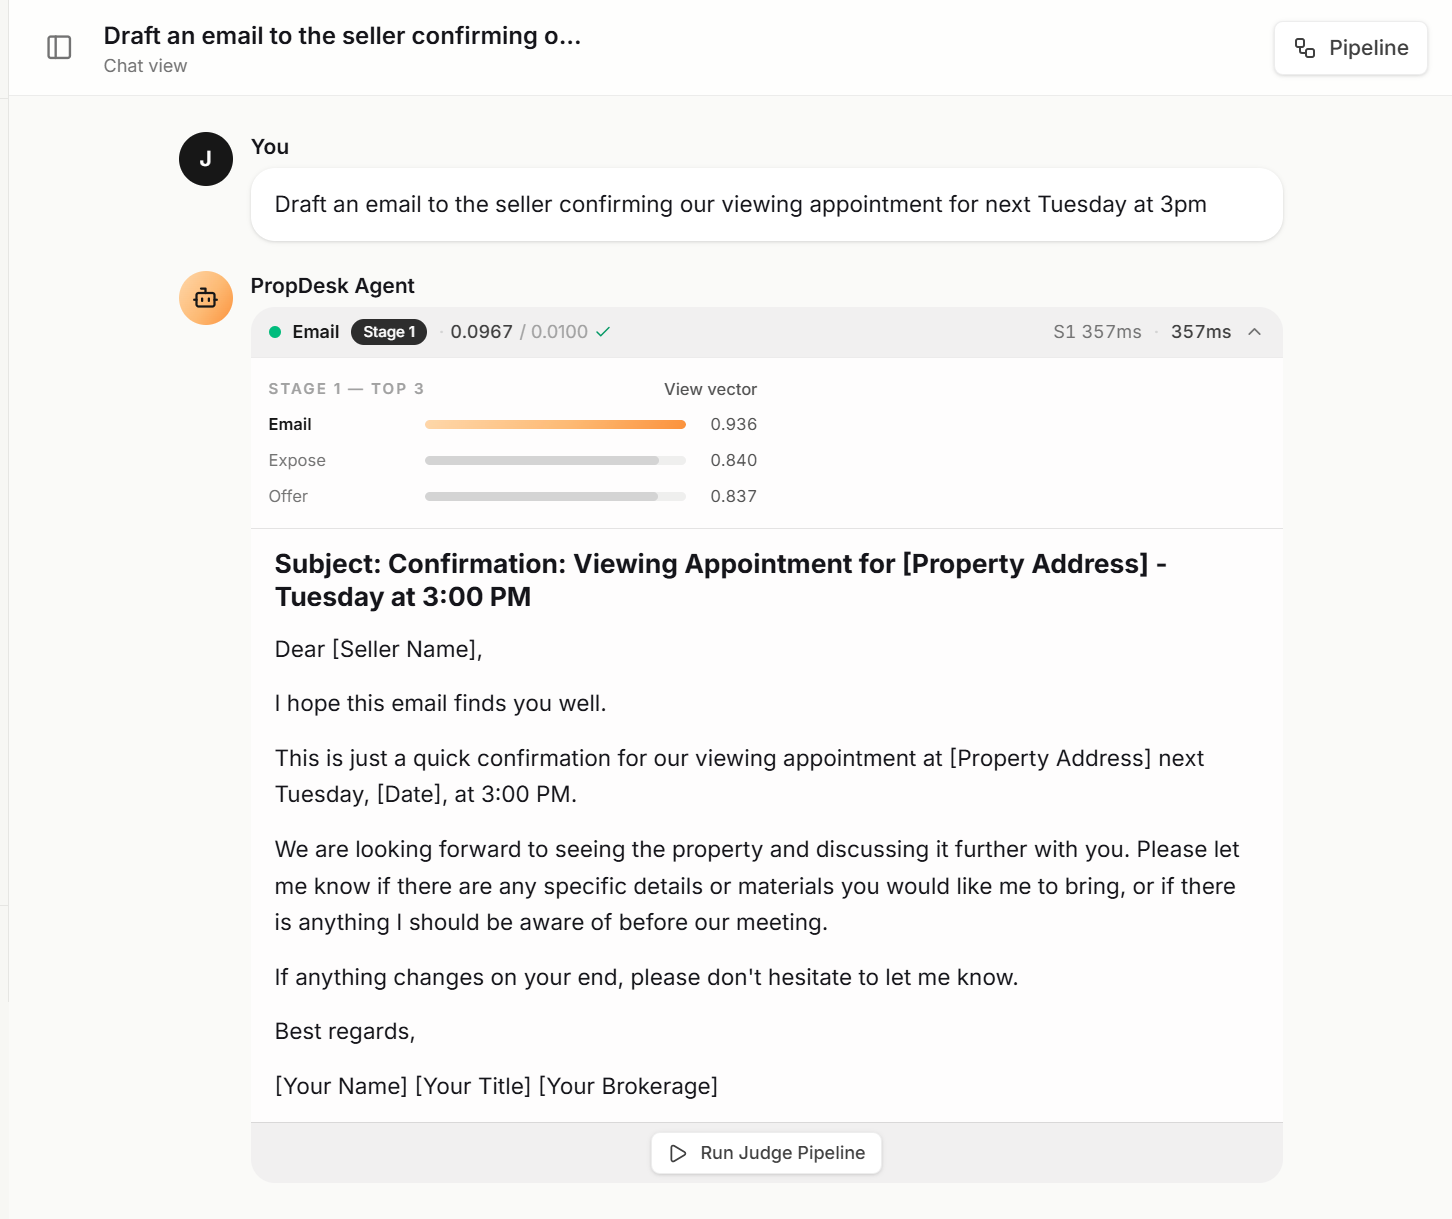
\includegraphics[width=0.7\linewidth,height=\textheight,keepaspectratio]{assets/sprints/sprint4-chat-view.png}
\caption{Chat view showing the routed agent, the Stage 1 routing decision, and the per-agent confidence scores.}\label{fig:sprint4-chat-view}
\end{figure}

\begin{figure}
\centering
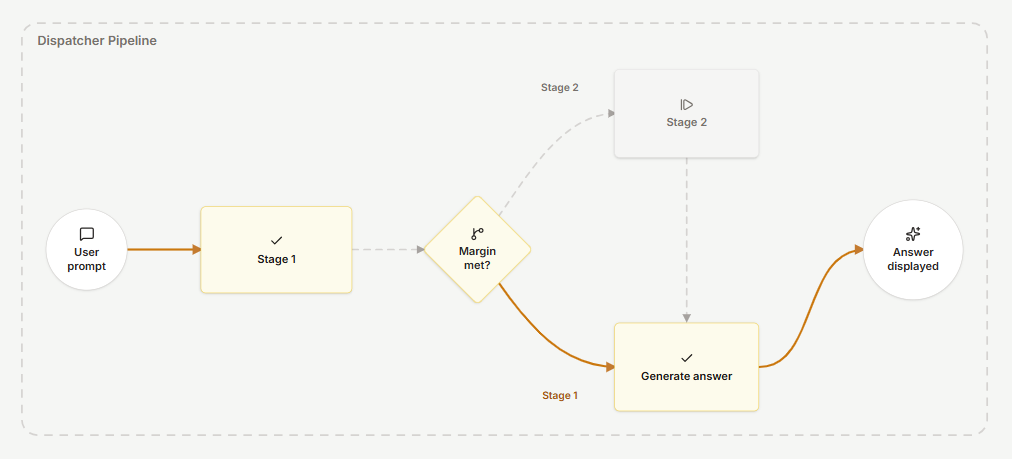
\includegraphics[width=1\linewidth,height=\textheight,keepaspectratio]{assets/sprints/sprint4-router-pipeline.png}
\caption{Router pipeline diagram, with the highlighted path showing a query routed directly by Stage 1 and Stage 2 left skipped.}\label{fig:sprint4-router-pipeline}
\end{figure}

The remaining architectural decision was the choice of optimizer. On a shared 548-example set covering all eight agents, DSPy MIPROv2 improved Stage 2 accuracy from 95.45 to 96.59 percent, a gain of 1.14 percentage points, but only once the dataset was large enough to expose a consistent signal. On the same data, OPRO reached 98.6 percent from a comparable baseline in six rounds. The difference lies in the optimization strategy: rather than searching statistically over a validation set, OPRO grounds its meta-prompt in judge-confirmed routing failures, refining the prompt from explicit failure cases instead of requiring broad coverage of the task distribution \autocite{yang2023llmoptimizers}. The team selected OPRO and aligned the decision with Julian and Rainer on 16 June. To measure improvement without bias, Gáspár then built a deliberately difficult ground-truth test dataset across all eight agents, held out from every optimization run.

\subsubsection{Sprint Review}\label{sec:sprint4-review}

The review took place on 23 June 2026 over Microsoft Teams with Julian and Rainer. After presenting the OPRO decision, the team ran the full pipeline end to end, from a query through routing and response to a judge evaluation. The highlight was a live demonstration of the self-improvement loop: because the judge had written new vector entries during the demo, the product owners asked whether a query that had previously required Stage 2 would now be handled by Stage 1 directly. It was, confirming in real time that the judge's corrections were improving routing. Julian raised a concern about the Stage 1 vector index growing over time, and the team pointed to the novelty check that prevents near-duplicate entries and proposed approximate nearest-neighbor search for scale. Both product owners gave their strongest endorsement so far, noting that the team now had a product worth presenting to a wider audience and advising it to step back in the final sprint to communicate what had been built rather than adding features.

The team completed all seven user stories and delivered the full 25 story points. The burndown (\cref{fig:sprint4-burndown}) stayed flat for much of the sprint and dropped sharply near the end, reflecting the nature of the integration work. The two largest tickets, the skeleton and dashboard, could only be closed once fully completed.

\begin{figure}
\centering
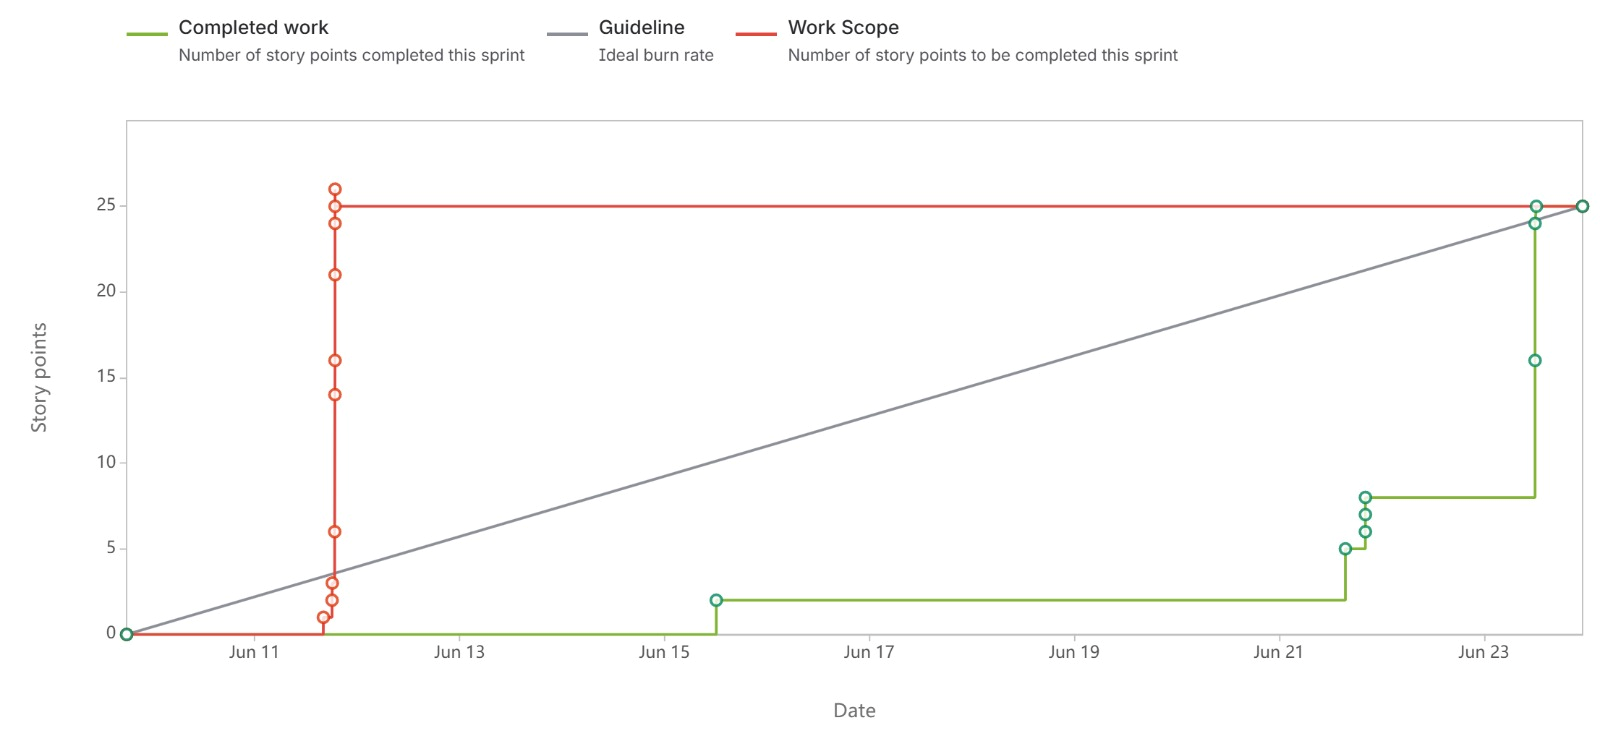
\includegraphics[width=1\linewidth,height=\textheight,keepaspectratio]{assets/sprints/sprint4-burndown.png}
\caption{Sprint 4 burndown chart, flat through the sprint and dropping as the two large integration tickets closed.}\label{fig:sprint4-burndown}
\end{figure}

\subsubsection{Sprint Retrospective}\label{sec:sprint4-retrospective}

The Sprint 4 retrospective used an adapted Sailboat format (\cref{fig:sprint4-sailboat}), based on a publicly available Miro template \autocite{miro2024sailboat}, chosen to keep the session engaging and frame the sprint within the wider project. Held on 23 June within a strict forty-minute timebox, it moved through four themes. Under Tailwinds the team credited coordination, planning together before building, and the increased meeting cadence. The Delights centered on the product finally feeling complete and ready to demonstrate, with the dashboard and the clarity of the optimizer decision singled out. The Restraints were personal rather than technical, dominated by exams and university stress, while the absence of any technical blocker was itself a signal that earlier integration friction had been resolved. The Future Risks looked ahead to the exam period as a capacity risk and to the challenge of making a complex product understandable to a broader audience, a shift from solving technical integration problems toward managing delivery risk and communication as the project approached completion.

\begin{figure}
\centering
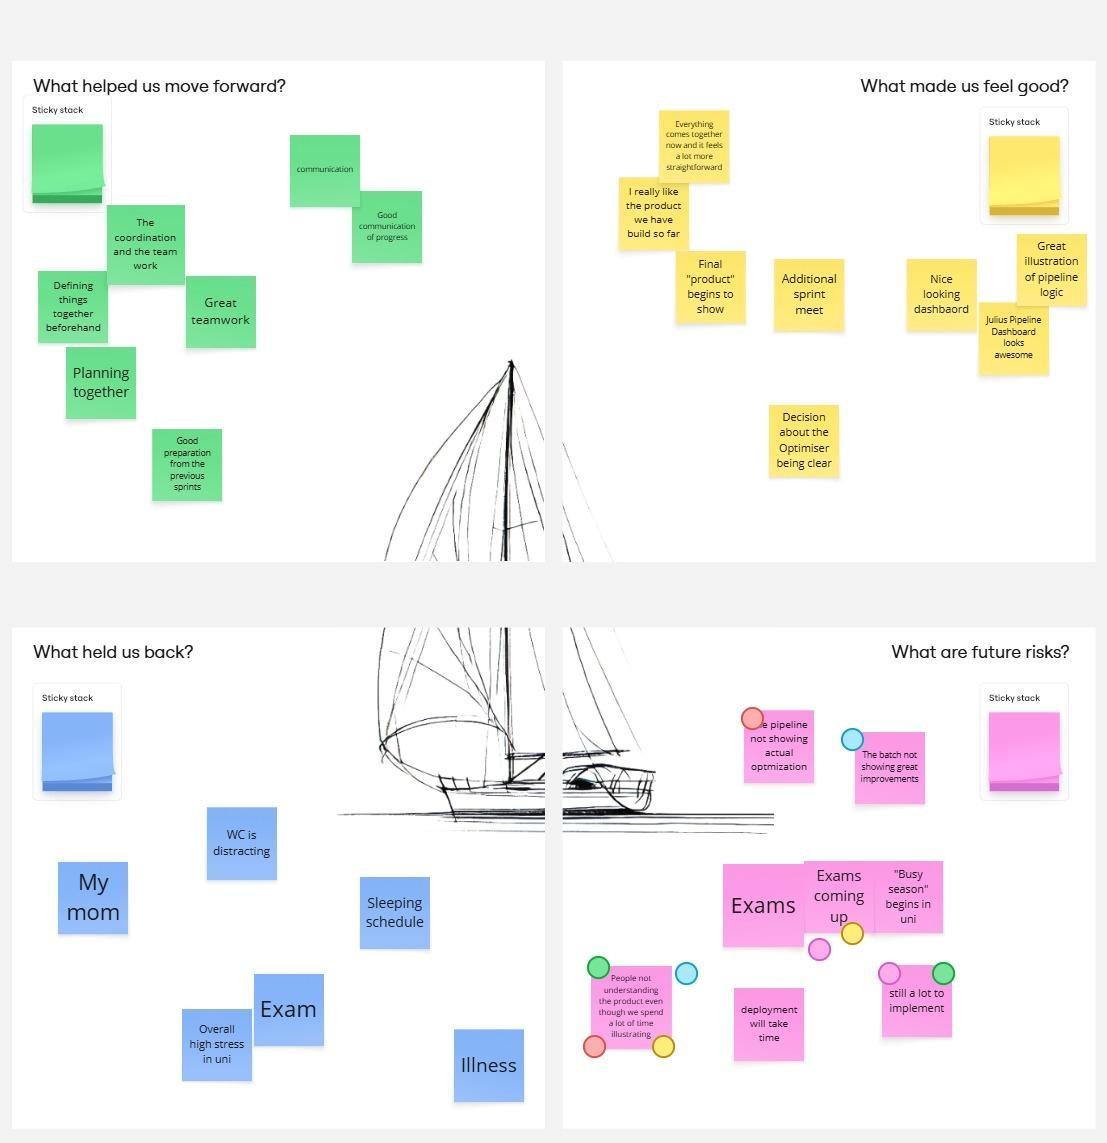
\includegraphics[width=0.65\linewidth,height=\textheight,keepaspectratio]{assets/sprints/sprint4-retrospective.jpg}
\caption{Sailboat retrospective board, with Tailwinds and Delights on the top row and Restraints and Future Risks below.}\label{fig:sprint4-sailboat}
\end{figure}

Two action items were adopted for Sprint 5. First, each member would block dedicated time around the exam period to protect the team's capacity for the final sprint, directly addressing the risk that had dominated the retrospective. Second, the team committed to delivering a well-defined dashboard by 30 June, the technical priority flagged as still outstanding. Both were assigned to the team as a whole rather than to individual owners, reflecting the collaborative nature of the final stretch (\cref{fig:sprint4-action-items}).

\begin{figure}
\centering
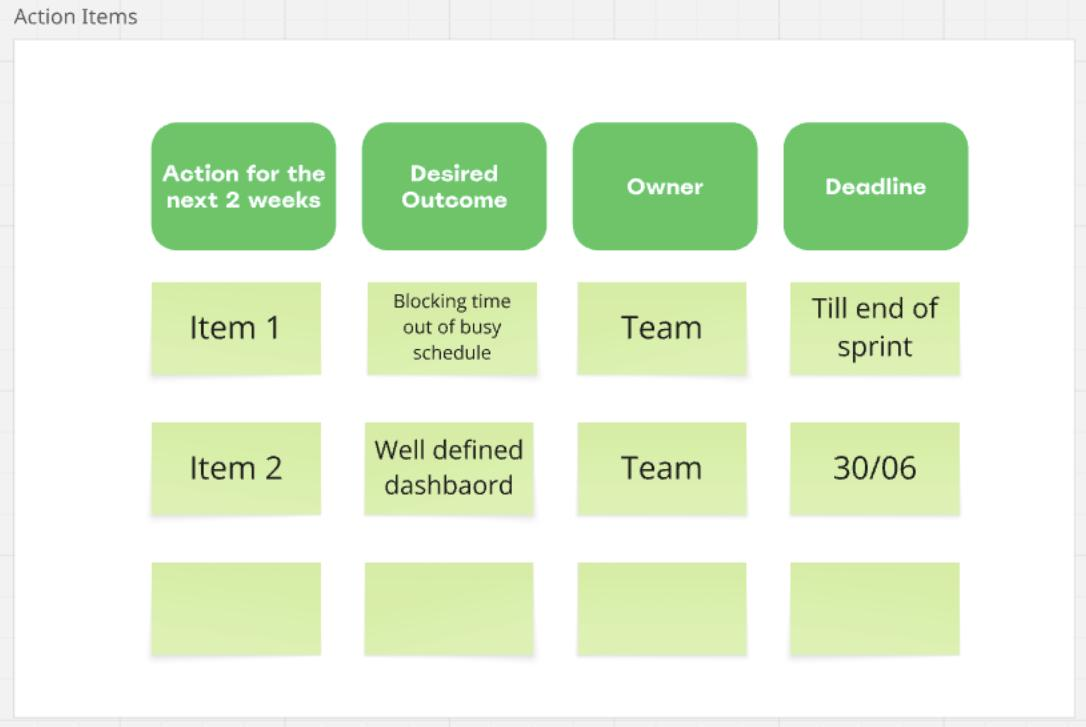
\includegraphics[width=1\linewidth,height=\textheight,keepaspectratio]{assets/sprints/sprint4-action-items.jpg}
\caption{The two action items agreed in the retrospective for Sprint 5: protecting team capacity during the exam period and delivering a well-defined dashboard by 30 June.}\label{fig:sprint4-action-items}
\end{figure}

\authoredsubsection{Sprint 5}{Sebastian}{Sebastian Straub}\label{sec:sprint5}

Sprint 5 ran from 23 June to 06 July 2026, with the review and retrospective held on 07 July, and closed the project. With the pipeline fully integrated at the end of Sprint 4, the character of the work changed. The focus shifted from building new capability toward proving the self-improvement loop end to end, making its performance visible to operators, and handing the system over to Interhyp in a state the team could walk away from. Sebastian Straub served as Scrum Master for this final sprint.

\subsubsection{Sprint Goals}\label{sec:sprint5-goals}

The sprint goal committed the team to running systematic batch evaluations of the full pipeline against the ground-truth test dataset, building a Batch-Running Dashboard and an Optimization Dashboard to make routing accuracy and optimization cycles visible, deploying the system, and preparing the final presentation, the handover document, and a knowledge transfer session for Interhyp. Behind these deliverables stood one measurable outcome, defined as Interhyp being able to operate, evaluate, and extend the pipeline independently by the end of the sprint. The goal was deliberately phrased around this outcome, since a final sprint that leaves a working yet unexplainable system behind would have missed the point of the engagement.

\subsubsection{Sprint Planning}\label{sec:sprint5-planning}

Planning started from two gaps left open after Sprint 4. The optimizer's execution flow was not yet visible in the frontend, and no dedicated view measured routing accuracy over time, which Interhyp had explicitly requested during the Sprint 4 review. The resulting backlog contained seven tickets totaling 25 story points, consistent with the velocity established over the previous sprints. The stand-up cadence of four meetings per week was kept unchanged, with the in-person Tuesday session continuing to anchor each week ahead of the Interhyp meeting.

\Cref{fig:sprint5-backlog} shows the resulting backlog. The Batch-Running Dashboard (five story points) lay with Sebastian Straub, the Optimization Dashboard (three) with Gáspár Harmati supported by Sebastian Straub, the Monitoring Dashboard (three) with Marco Schröder, System Deployment (five) with Julius Bethge, the Handover Document (two) with Gáspár Harmati, and the Knowledge Transfer Session (two) with Mohsin Saeed. The Final Presentation (five) was split into one subtask per team member and coordinated by Mohsin Saeed, since it had to bring the work of all five into one consistent story.

\begin{figure}
\centering
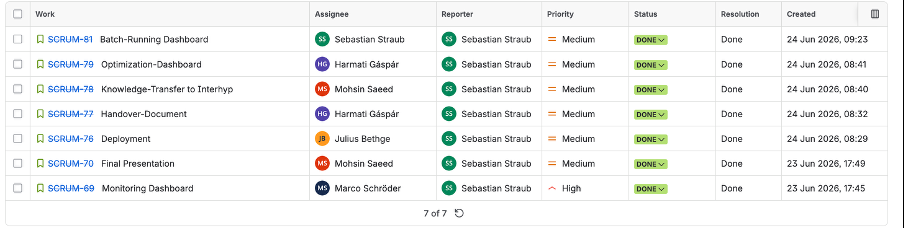
\includegraphics[width=1\linewidth,height=\textheight,keepaspectratio]{assets/sprints/sprint5-backlog.png}
\caption{Sprint 5 backlog showing owners and completion status (Jira).}\label{fig:sprint5-backlog}
\end{figure}

\subsubsection{Implementation and Execution}\label{sec:sprint5-execution}

The sprint delivered three operator-facing dashboards on top of the existing chat and pipeline views. The Training Dashboard produces the labeled data the optimizer learns from. It runs an uploaded dataset through the full router, has the LLM judge score every routing decision, and reports accuracy, Stage 1 share, and cost per run. The Evaluation Dashboard measures a prompt version against a fixed held-out dataset and compares two versions side by side, down to a per-agent breakdown, a confusion matrix, and a diff of the exact prompt text that changed. The Optimization Dashboard makes the OPRO loop watchable in real time, plotting the score of every candidate prompt in every round. The Monitoring Dashboard complements them with an operations view of query volume, cost, Stage 1 share, and per-agent accuracy over time. All views stream their data over the same reactive Convex connection that powers the chat, so results appear live without any refresh.

Several operational details determine how these views hold up in day-to-day use. Every training run is preserved as its own record, labeled with the prompt version it ran under, so operators can compare how one dataset performed across prompt versions without re-running anything. Long runs can be stopped from the dashboard, and the worker picks the signal up within a few processed items and terminates cleanly. Evaluation runs skip answer generation entirely, since only the routing decision is measured, which makes each evaluation call faster and cheaper than a full dispatch. The optimization view plots the seed prompt, the best score per round, and every individual candidate, and once a champion prompt is deployed it shows the previous and the new version side by side with the changed lines highlighted. The Monitoring Dashboard is fully wired to the backend but currently displays simulated demo data, since PropDesk has not yet processed real broker traffic, and it will fill with live data without further changes once it does.

The methodologically most important work of the sprint sits beneath these views. Undetected leakage between training and evaluation data is among the most common causes of overoptimistic results in machine-learning-based science \autocite{kapoor2023}, and contaminated benchmarks inflate reported LLM accuracy in the same way \autocite{sainz2023}. The pipeline therefore enforces the separation of training and evaluation data at four independent points. The Training Dashboard strips any prompt that also appears in the evaluation set before an upload reaches the backend, every batch run is tagged as train or eval in the database and filtered at query level, the optimizer's data selector can only ever access training runs, and a server-side guard rejects any attempt to reclassify an evaluation run. This is what allows the Stage 1 thresholds in \cref{sec:router-stage1} to be calibrated on data the reference store has never seen. Without it the accuracy figures in \cref{sec:empirical-evaluation} could not be read as a measurement of routing quality.

Deployment made PropDesk available at a public URL, with sign-in through Google SSO and an email whitelist, and completed the architecture shown in \cref{fig:sprint5-architecture}. A React frontend served from a CDN communicates with Convex, which acts as database, vector store, and job queue at once, while a long-running Python worker polls for jobs and executes the router, judge, and optimizer pipelines. A single environment variable switches the pipeline between a fully local mode, a production mode that routes judge and optimizer through AWS Bedrock in the eu-central-1 region to satisfy Interhyp's EU data residency requirement, and an OpenRouter mode for environments that cannot host models locally.

% Tall, dense diagram: give it a dedicated float page instead of letting it
% claim three quarters of a text page and leave the rest empty.
\begin{figure}[p]
\centering
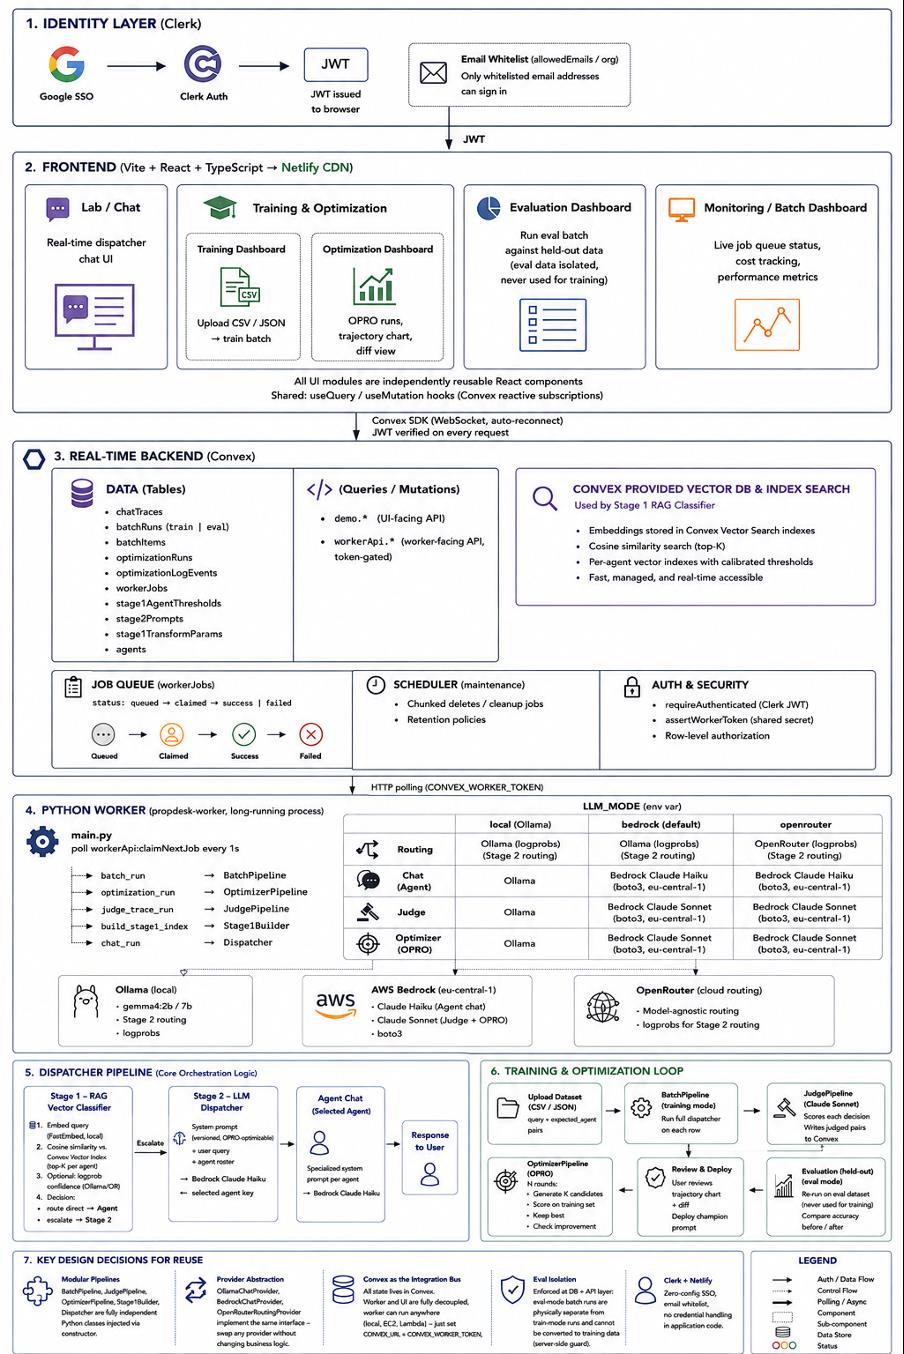
\includegraphics[width=0.95\linewidth,height=0.88\textheight,keepaspectratio]{assets/sprints/sprint5-deployment-architecture.png}
\caption{PropDesk deployment architecture across the identity, frontend, backend, and worker layers (own illustration).}\label{fig:sprint5-architecture}
\end{figure}

A final revision concerned the Stage 1 decision rule. The per-agent margin thresholds from Sprint 3 (\cref{sec:sprint3-execution}) decided escalation on the raw distance between the best and second-best agent score. This worked, but a margin is not comparable across agents and cannot be read as a probability, which made the threshold dashboard hard to interpret and the operating point hard to communicate to Interhyp. Stage 1 was therefore reworked onto a temperature-scaled softmax over the per-agent scores, with the thresholds refitted on the resulting top-agent probability \autocite{guo2017}. Temperature scaling is monotone and cannot alter the agent ranking, so the change affected only the abstention decision. The coverage and risk figures in \cref{sec:router-stage1} are those of the recalibrated configuration and supersede the Sprint 3 values.

The remaining tickets packaged the project for the time after the team. A handover document in C4 style records the architecture together with the decision records behind it, a knowledge transfer session backed by a written operator manual enables Interhyp's data scientists to run the system without the original team, and the final presentation was rebuilt around a simpler narrative after the mid-term feedback had shown that the story was getting lost in technical detail. A sprint-internal midterm presentation on 30 June served as a checkpoint, at which the functional Batch-Running Dashboard and the monitoring views were demonstrated and the remaining to-dos were consolidated.

\subsubsection{Sprint Review}\label{sec:sprint5-review}

The review on 07 July 2026 doubled as the project's final stakeholder meeting. The team presented the results of a final batch run, which reached 98 percent routing accuracy with 78 percent of all queries resolved by Stage 1 alone, compared to 83 percent accuracy and no Stage 1 index at the start of the project. Stage 1 was correct on 97 percent of the queries it accepted, inside the five percent error budget its thresholds were calibrated against. Every escalated query was routed correctly by Stage 2. \Cref{sec:empirical-evaluation} reports the full evaluation behind these figures. Interhyp's representatives walked through the deployed product and the new dashboards, congratulated the team on a project they called a success, and highlighted that the solutions were grounded in the literature rather than improvised. Beyond the dashboards, the session included a short exchange on fine-tuning individual parts of the system and a preview of the final presentation concept, so Interhyp knew what to expect ahead of the joint final session. Only two backlog items were deferred beyond the project, a sampling table that would spread judge coverage more evenly across agents and file upload support for queries, and neither affects the delivered functionality.

The burndown chart of this sprint requires interpretation (\cref{fig:sprint5-burndown}). It stays flat for most of the sprint and collapses on the final day, which reflects a tracking convention rather than the actual flow of work. Finished tickets were parked in a To Be Verified column until Interhyp confirmed the deliverables during the review, and only then moved to Done. A stricter reading of Scrum would have closed tickets as soon as the work was done instead of gating closure on a meeting that happens once per sprint, and the chart would then show the steady decline that actually took place. Several estimates also proved too low, since consolidating five sprints of work into one deployed and documented artifact multiplied effort in ways the individual tickets did not capture. The team chose to absorb this in a demanding final stretch rather than descoping work.

\begin{figure}
\centering
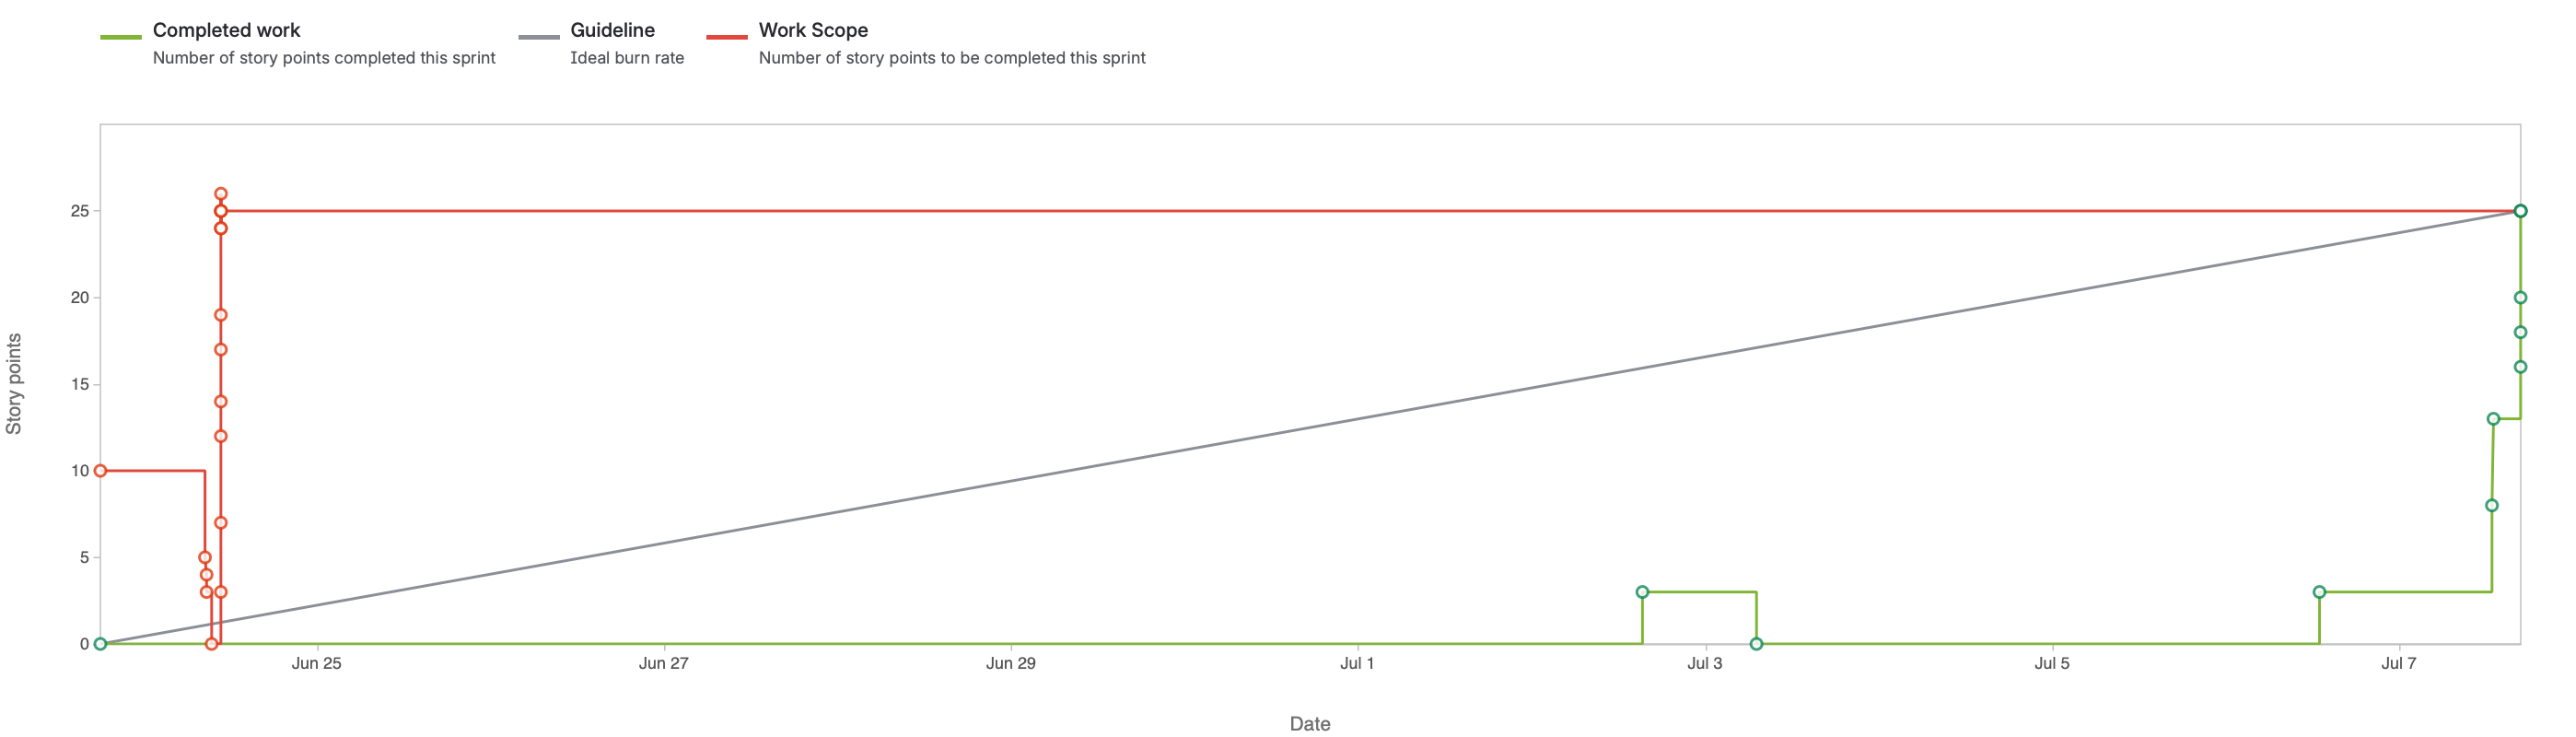
\includegraphics[width=1\linewidth,height=\textheight,keepaspectratio]{assets/sprints/sprint5-burndown.png}
\caption{Sprint 5 burnup chart (Jira).}\label{fig:sprint5-burndown}
\end{figure}

\subsubsection{Final Retrospective}\label{sec:sprint5-retrospective}

Since no next sprint remained to derive action items for, the team replaced the usual retrospective format with a retrospective across the full twelve weeks, held in person on a Miro board built for the occasion (\cref{fig:sprint5-retrospective}). In the team's own assessment, what carried the project were the discipline of sticking to the Scrum plan, the consistently good mood, and the collaboration with Interhyp. What ran less smoothly were coordinating five personal schedules, applying Scrum rigidly to work that was at times research-heavy rather than feature-shaped, and the recurring friction of exhausting LLM token budgets during training runs. The biggest learnings were that a substantial project is achievable within twelve weeks when a team commits to it, that coordinating a university project across individual schedules is harder than coordinating work in a professional context, and that stepping back early beats getting stuck in details. Asked what it would do differently, the team named more open communication from the start, more in-person sessions, and a looser application of Scrum where the work did not call for its full structure. None of this changed the closing sentiment of the session, which was pride in the collaboration and in the product handed over.

\begin{figure}
\centering
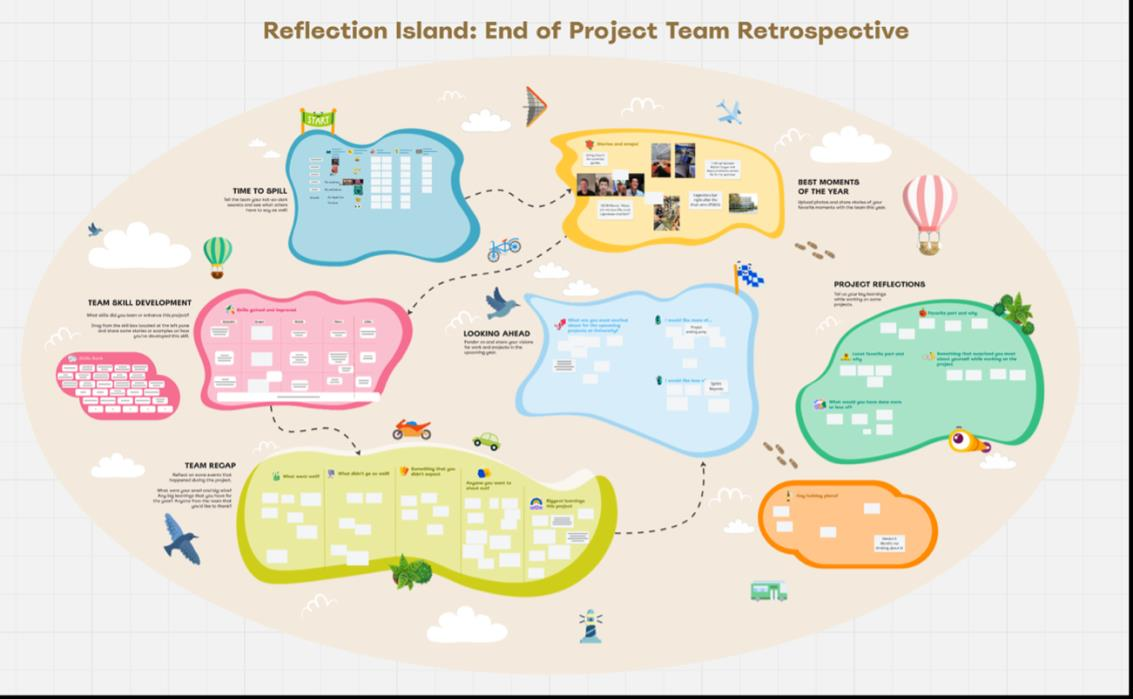
\includegraphics[width=1\linewidth,height=\textheight,keepaspectratio]{assets/sprints/sprint5-retrospective.png}
\caption{Final project retrospective board (Miro).}\label{fig:sprint5-retrospective}
\end{figure}



\clearpage
\suppressfloats[t]
\clearreportauthor
\section{Empirical Evaluation}\label{sec:empirical-evaluation}

\pendingcontent{Empirical evaluation results}{Insert the finalized experimental design and results. Keep datasets and baselines separated, report accuracy, latency, cost, Stage 1 coverage, optimization effects, judge reliability, and error analysis with the corresponding figures and tables.}


\clearpage
\suppressfloats[t]
\authoredsection{Project Review}{Mohsin}{Mohsin Saeed}\label{sec:project-review}

\subsection{Challenges and Solutions}\label{sec:challenges}

The project faced three main practical constraints. Each was met with a deliberate workaround rather than a compromise on scope.

\subsubsection{No Dedicated Budget for Frontier Models}\label{sec:challenge-budget}

The pipeline depended heavily on language models. Stage 2 routing, the judge, and the optimizer all required repeated LLM calls, but the project had no budget allocated for frontier models. To keep development moving, we used Ollama to run open-source models locally. While this allowed us to build and test the pipeline without any cost, the available models were smaller and significantly slower than frontier models, making them unsuitable for large-scale judging and optimization experiments. Later in the project, we secured AWS Bedrock credits, providing access to models such as Claude Haiku and Claude Sonnet. This allowed us to combine the strengths of both approaches: Ollama for fast local development and Bedrock for the more demanding evaluation and optimization workloads. As a result, we were able to complete all experiments without incurring API costs.

\subsubsection{No Production Data}\label{sec:challenge-data}

Since Interhyp could not share production customer queries, there was no real-world dataset available for training or evaluating the pipeline. Instead, they provided the distribution of queries across the eight specialist agents, allowing us to construct datasets that reflected the expected workload. Rather than relying on a single dataset, we generated multiple datasets with increasing levels of difficulty, ranging from straightforward single-domain questions to complex multi-domain queries containing spelling mistakes and noisy copy-paste text. Evaluating the pipeline across this range provided a much clearer picture of its strengths and weaknesses than testing on only one type of data.

\subsubsection{An Inherently Complex System}\label{sec:challenge-complexity}

Unlike projects built around a single model, this one required several interconnected modules, the router, the judge, and the optimizer, each with its own logic but all needing to work together. Building this pipeline as one piece of software would have made debugging and testing far harder, so we used a modular architecture, developing and testing each component independently before integrating it. This kept the complexity manageable and let each part evolve without destabilizing the rest. The same complexity made the system hard to explain. With so many components interacting before a result appears, the full workflow was difficult to follow for anyone seeing it for the first time. To address this, we built a visual demonstration showing a query moving through each stage, and used a football analogy in the presentation to explain each component's role. This made the system easier to follow while still accurately representing its underlying complexity.

\subsection{Limitations}\label{sec:limitations}

While the project achieved its intended goals, several limitations remain due to the scope of the evaluation and the constraints under which the system was developed.

The most significant limitation is that the evaluation relied entirely on synthetic data. Although the datasets were designed based on the query distribution across the eight agents and deliberately covered different levels of difficulty, they can only approximate real broker traffic. The system was never evaluated with live user queries. Therefore, the reported accuracy values should be interpreted as promising but not yet representative of production performance. The pipeline's long-term behavior, performance under real traffic, and production latency still need to be validated on real data.

A second limitation is that the self-improvement loop relies on a single judge. While the judge currently achieves 99\% agreement with the ground truth, this does not mean it is guaranteed to be error-free. The concern is structural: because every correction to the router comes from this one component, its mistakes have nowhere to be caught. Any error the judge makes would feed straight into the Stage 1 store and the optimizer and shape the router from there.

Finally, the pipeline was evaluated on a limited range of models: local models served through Ollama, and Claude Haiku and Claude Sonnet through Bedrock. The behavior of the system may differ when using other providers, model families, or model sizes. Therefore, the findings are limited to the specific models and configurations evaluated in this project.

\subsection{Potential Enhancements}\label{sec:enhancements}

The project established several directions for future improvement. Two of these enhancements were already explored during the final sprint, while the remaining opportunities build on limitations identified during evaluation.

\subsubsection{Monitoring Dashboard}\label{sec:enhancement-dashboard}

To give Interhyp visibility into the system in production, the team built a monitoring dashboard (\cref{fig:monitoring-dashboard}). It provides a single view of key system metrics, including router accuracy, query volume, the proportion of queries resolved directly by Stage 1, average latency, and LLM costs. The dashboard and supporting data pipeline are already implemented; however, it currently displays demo data because the system has not yet received live traffic. Every chart would fill with real data automatically once queries begin to flow. The remaining step is deploying it against live production traffic, at which point it would let Interhyp track accuracy, cost, and index growth over time and catch drift or regressions early, closing the gap left by evaluating the system only offline.

\begin{figure}
\centering
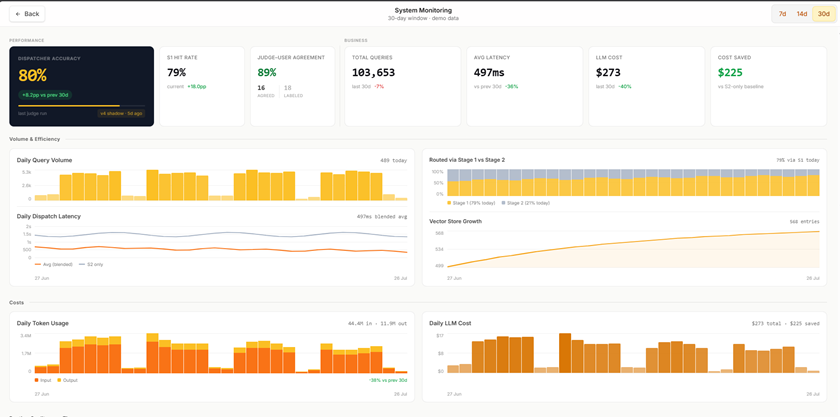
\includegraphics[width=0.85\linewidth,height=\textheight,keepaspectratio]{assets/review/monitoring-dashboard.png}
\caption{The monitoring dashboard, shown with demo data pending live traffic, giving a single operator-facing view of accuracy, the Stage 1 and Stage 2 routing split, latency, volume, vector-index growth, and cost.}\label{fig:monitoring-dashboard}
\end{figure}

\subsubsection{Human in the Loop}\label{sec:enhancement-hitl}

The judge currently provides the feedback signal that drives the improvement loop without human verification. A human-in-the-loop approach would introduce human validation alongside the automated judge. The team sketched a concept for this (\cref{fig:human-in-the-loop}): an interface that presents two candidate answers side by side so a reviewer can choose the more helpful one, extended in future by a lightweight thumbs up or down control on individual answers. Signals collected this way would give an independent check on the judge's verdicts and a source of high-confidence labels, so the automated judge is no longer the only source of truth. This remains a proposed design rather than an implemented feature.

\begin{figure}
\centering
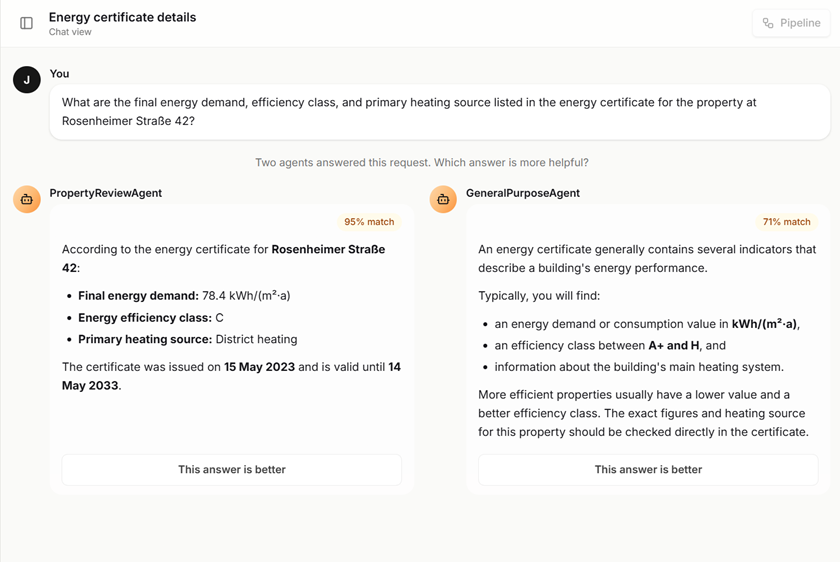
\includegraphics[width=0.85\linewidth,height=\textheight,keepaspectratio]{assets/review/human-in-the-loop.png}
\caption{Concept design for a human-in-the-loop review step, in which a reviewer selects the more helpful of two answers. Proposed, not yet implemented.}\label{fig:human-in-the-loop}
\end{figure}

\subsubsection{Hyperparameter Tuning}\label{sec:enhancement-hyperparameters}

Several values in the current system are manually configured, the number of candidate agents the judge compares, and optimizer settings such as the number of rounds and candidates. These values could instead be treated as tunable hyperparameters and optimized using Interhyp's own data and objectives. This would allow the system to be calibrated according to their priorities, balancing accuracy, latency, and cost rather than relying on values selected under the project's time constraints.

\subsubsection{Judge}\label{sec:enhancement-judge}

As the limitations already indicated, although the judge reached 99\% agreement on the evaluation dataset, it is not guaranteed to be error free on new production queries. It will be required in the future to test the judge's reliability periodically with a ground truth dataset constructed out of new queries. If the judge agreement rate on this dataset drops significantly, setting up a judge panel would be the most reasonable next step.

Furthermore, we investigated using the judge model's log probabilities as a confidence signal to quantify how certain the judge was about a given verdict rather than only obtaining a binary decision and its reasoning. Such a signal could be compared against the router's own confidence in its routing decision to estimate the size of the resulting error signal or used to flag particularly uncertain cases for human review, strengthening the human-in-the-loop approach. This did not prove feasible with GPT-OSS-120B, the model used for this exploration via the AWS Bedrock API. As a reasoning model, it commits to its decision internally before generating the visible output token, so the extracted log probabilities were consistently 100\% for one candidate and 0\% for the other, regardless of how close the actual decision was. The approach may still be viable with non-reasoning models that expose meaningful log probabilities, and remains worth revisiting when different models are available.


\clearpage
\suppressfloats[t]
\clearreportauthor
\section{Conclusion}\label{sec:conclusion}

This project achieved its objective of designing, implementing, and evaluating a reproducible pipeline for improving the routing of a multi-agent chatbot. The resulting system integrates a selective similarity-based Stage 1 Router, an LLM-based Stage 2 Router, an LLM judge, and an OPRO-based prompt optimizer in a working showcase application. The accompanying dashboards make the evaluation, training, optimization, and deployment workflow inspectable rather than leaving prompt improvement as an ad hoc manual process.

The controlled evaluation provides evidence that the approach can improve the agreed performance dimensions. On the fixed 240-query evaluation dataset, optimizing the Stage 2 prompt increased routing accuracy from 83\% to 100\%. The complete two-stage Router achieved 98\% accuracy, routed 78\% of queries without a Stage 2 LLM call, and reduced average latency from 669 ms to 407 ms. It therefore retained most of the accuracy gain while lowering model use and latency. At the same time, the difference between judge-based and golden-label results shows that automated feedback is useful for optimization but should not be treated as perfectly calibrated ground truth.

The findings remain subject to the project's main limitations: all experiments used synthetic data, the improvement loop relied on a single judge, and only a limited set of models and configurations was tested. The results therefore demonstrate technical feasibility in the showcase environment, not production performance at Interhyp. A next step should validate the pipeline on independently labelled production samples, monitor accuracy, latency, and cost under live traffic, and introduce periodic human review or a judge panel if reliability declines. With these safeguards, the implemented pipeline offers Interhyp a practical foundation for replacing case-by-case Router refinement with a systematic and measurable improvement process.


\clearpage
\clearreportauthor
\printbibliography[heading=bibintoc,title={List of references}]

\clearpage
\section*{Overview of Tools Used}

\begingroup
\small
\setlength{\tabcolsep}{4pt}
\renewcommand{\arraystretch}{1.3}
\begin{longtable}{|
  >{\raggedright\arraybackslash}p{0.19\textwidth}|
  >{\raggedright\arraybackslash}p{0.17\textwidth}|
  >{\raggedright\arraybackslash}p{0.37\textwidth}|
  >{\raggedright\arraybackslash}p{0.18\textwidth}|}
\hline
\rowcolor{gray!20}
\textbf{Technology Utilized} &
\textbf{Declared Objective} &
\textbf{Operational Application} &
\textbf{Degree of Integration} \\
\hline
\endfirsthead
\hline
\rowcolor{gray!20}
\textbf{Technology Utilized} &
\textbf{Declared Objective} &
\textbf{Operational Application} &
\textbf{Degree of Integration} \\
\hline
\endhead
Claude Code (Opus 4.8, Fable 5) &
Coding assistance &
Used to support implementation, debugging, refactoring, and code-related documentation. All generated code was reviewed by project members before integration and modified manually wherever necessary. &
Regularly during software development \\
\hline
Codex (GPT 5.5, GPT 5.6 Sol) &
Coding assistance &
Used to support implementation, debugging, refactoring, and code-related documentation. All generated code was reviewed by project members before integration and modified manually wherever necessary. &
Regularly during software development \\
\hline
Gemini &
Proofreading and idea clarification &
Used to review wording and readability and to clarify ideas during drafting. Suggestions were assessed by the authors and incorporated selectively. &
Selectively during drafting and final review \\
\hline
\end{longtable}
\endgroup


\clearpage
\hypersetup{pageanchor=false}
\pagenumbering{Roman}
\setcounter{page}{1}
\section*{Declaration of Authenticity}

% Official wording:
% https://cms-cdn.lmu.de/media/15-soziologie/studium/ma-eigenstandigkeitserklarung_en.pdf
I hereby declare that I have written this Master thesis independently and without outside
assistance, that I did not use any other sources apart from the ones stated in the bibliography
and that I have clearly cited all passages in my work that were taken from other sources. This
Master thesis has never been previously submitted in its current or similar form in any other
course and/or degree program. I agree that the examiner can electronically check my work by
using the appropriate software.

\vspace{1.5cm}
\submissionplace, \submissiondate

\newcommand{\insertsignature}[1]{%
  \IfFileExists{assets/signatures/#1.png}{%
    \includegraphics[width=0.85\linewidth,height=1.25cm,keepaspectratio]{assets/signatures/#1.png}%
  }{%
    \IfFileExists{assets/signatures/#1.jpg}{%
      \includegraphics[width=0.85\linewidth,height=1.25cm,keepaspectratio]{assets/signatures/#1.jpg}%
    }{%
      \IfFileExists{assets/signatures/#1.jpeg}{%
        \includegraphics[width=0.85\linewidth,height=1.25cm,keepaspectratio]{assets/signatures/#1.jpeg}%
      }{%
        \IfFileExists{assets/signatures/#1.pdf}{%
          \includegraphics[width=0.85\linewidth,height=1.25cm,keepaspectratio]{assets/signatures/#1.pdf}%
        }{}%
      }%
    }%
  }%
}

\newcommand{\signatureblock}[2]{%
  \begin{minipage}[t]{0.46\textwidth}
    \centering
    \begin{minipage}[c][1.4cm][c]{0.9\linewidth}
      \centering
      \insertsignature{#1}
    \end{minipage}\par
    \rule{0.9\linewidth}{0.4pt}\par
    {\small #2}
  \end{minipage}%
}

\vspace{0.8cm}
\noindent
\signatureblock{julius-bethge}{Julius Bethge}
\hfill
\signatureblock{gaspar-harmati}{G\'asp\'ar Harmati}

\vspace{0.8cm}
\noindent
\signatureblock{mohsin-saeed}{Mohsin Saeed}
\hfill
\signatureblock{marco-fabian-schroeder}{Marco-Fabian Schr\"oder}

\vspace{0.8cm}
\begin{center}
  \signatureblock{sebastian-straub}{Sebastian Straub}
\end{center}


\end{document}
